\subsection{Hiện thực hệ thống}

\textbf{Link github dự án}: \href{https://github.com/dasabu/matchjob-dbms-asgmt-version}{https://github.com/dasabu/matchjob-dbms-asgmt-version}\\

\textbf{Chạy dự án (môi trường local)}:
\begin{enumerate}
    \item Clone dự án: \texttt{git clone https://github.com/dasabu/matchjob-dbms-asgmt-version}
    \item Chạy back-end:
    \begin{itemize}
        \item Chuyển đến thư mục \texttt{backend}: \texttt{cd backend}
        \item Cài đặt các dependencies cần thiết: \texttt{npm install}
        \item Start server: \texttt{npm run start:dev}
    \end{itemize}
    \item Chạy front-end:
    \begin{itemize}
        \item Chuyển đến thư mục \texttt{frontend}: \texttt{cd frontend}
        \item Cài đặt các dependencies cần thiết: \texttt{npm install}
        \item Start client:
        \texttt{npm run dev}
    \end{itemize}

    \item Truy cập vào ứng dụng:
    \begin{itemize}
        \item Backend: \texttt{http://localhost:3333}
        \item Frontend: \texttt{http://localhost:3004}
    \end{itemize}
\end{enumerate}

\textbf{Lưu ý}: Cần phải cài đặt \href{https://nodejs.org/en}{\textbf{Node.js Runtime}} và \href{https://www.mongodb.com/docs/manual/installation/}{\textbf{MongoDB}} để chạy được dự án

% \subsubsection{Kết nối Backend - Database}

Trong hệ thống backend, nhóm tạo một module riêng biệt được dùng cho việc quản lý kết nối và truy cập đến cơ sở dữ liệu là \textbf{MongoModule}. Trong module này, \textbf{MongoService} là service được nhóm định nghĩa nhằm khởi tạo kết nối với database của hệ thống khi module khởi chạy và cung cấp đối tượng \texttt{Db} (đại diện cho cơ sở dữ liệu của hệ thống), thông qua một phương thức chung \texttt{getDatabase} cho các service khác sử dụng.

\begin{lstlisting}
import { Injectable, OnModuleDestroy, OnModuleInit } from '@nestjs/common';
import { MongoClient, Db } from 'mongodb';

@Injectable()
export class MongoService implements OnModuleInit, OnModuleDestroy {
    private client: MongoClient;    // Object MongoClient de quan ly ket noi
    private db: Db;                 // Object Db de truy cap vao database

    // Khoi tao ket noi khi module duoc khoi chay
    async onModuleInit() {
        const uri = process.env.MONGO_URI;
        const dbName = process.env.MONGO_DB_NAME;
        
        this.client = new MongoClient(uri);
        await this.client.connect();
        this.db = this.client.db(dbName);
        console.log(`Connected to MongoDB: ${dbName}`);
    }

    // Cung cap database cho cac module khac
    getDatabase(): Db {
        if (!this.db) {
          throw new Error('Database connection is not initialized');
        }
        return this.db;
    }

    // Dong ket noi khi module bi huy
    async onModuleDestroy() {
        await this.client.close();
        console.log('Disconnected from MongoDB');
    }
}
\end{lstlisting}

Khi đó, các module khác sẽ sử dụng \textbf{MongoService} đã khai báo ở trên để truy cập trực tiếp vào cơ sở dữ liệu của hệ thống để thực hiện các truy vấn cần thiết. Ví dụ, \textbf{JobsService} (nơi xử lý logic nghiệp vụ liên quan đến các thực thể công việc của hệ thống) sẽ \textbf{import} \textbf{MongoService} vào và thực hiện truy vấn "Danh sách các công việc đang tuyển dụng":

\begin{lstlisting}
import { Injectable, OnModuleInit } from '@nestjs/common';
import { Db } from 'mongodb';
import { MongoService } from './mongo.service';

@Injectable()
export class JobsService implements OnModuleInit {
    private db: Db;
    constructor(private mongoService: MongoService) {}
    
    // Khoi tao database tu MongoService khi module khoi chay
    onModuleInit() {
        this.db = this.mongoService.getDatabase();
    }
    
    // Vi du: Tra ve tat ca cac cong viec dang tuyen dung
    async getAllJobs() {
        return this.db      // Truy cap vao CSDL cua he thong
        .collection('jobs') // Truy cap vao collection 'jobs'
        .find({})           // Tim tat ca cac cong viec
        .toArray();         // Chuyen ket qua ve dang mang
    }
}
\end{lstlisting}

% \subsubsection{Giao diện người dùng - Trang chủ}

Trang chủ của website cung cấp thông tin trực quan, đầy đủ về các công việc mới nhất như sau:

\begin{figure}[H]
    \centering
    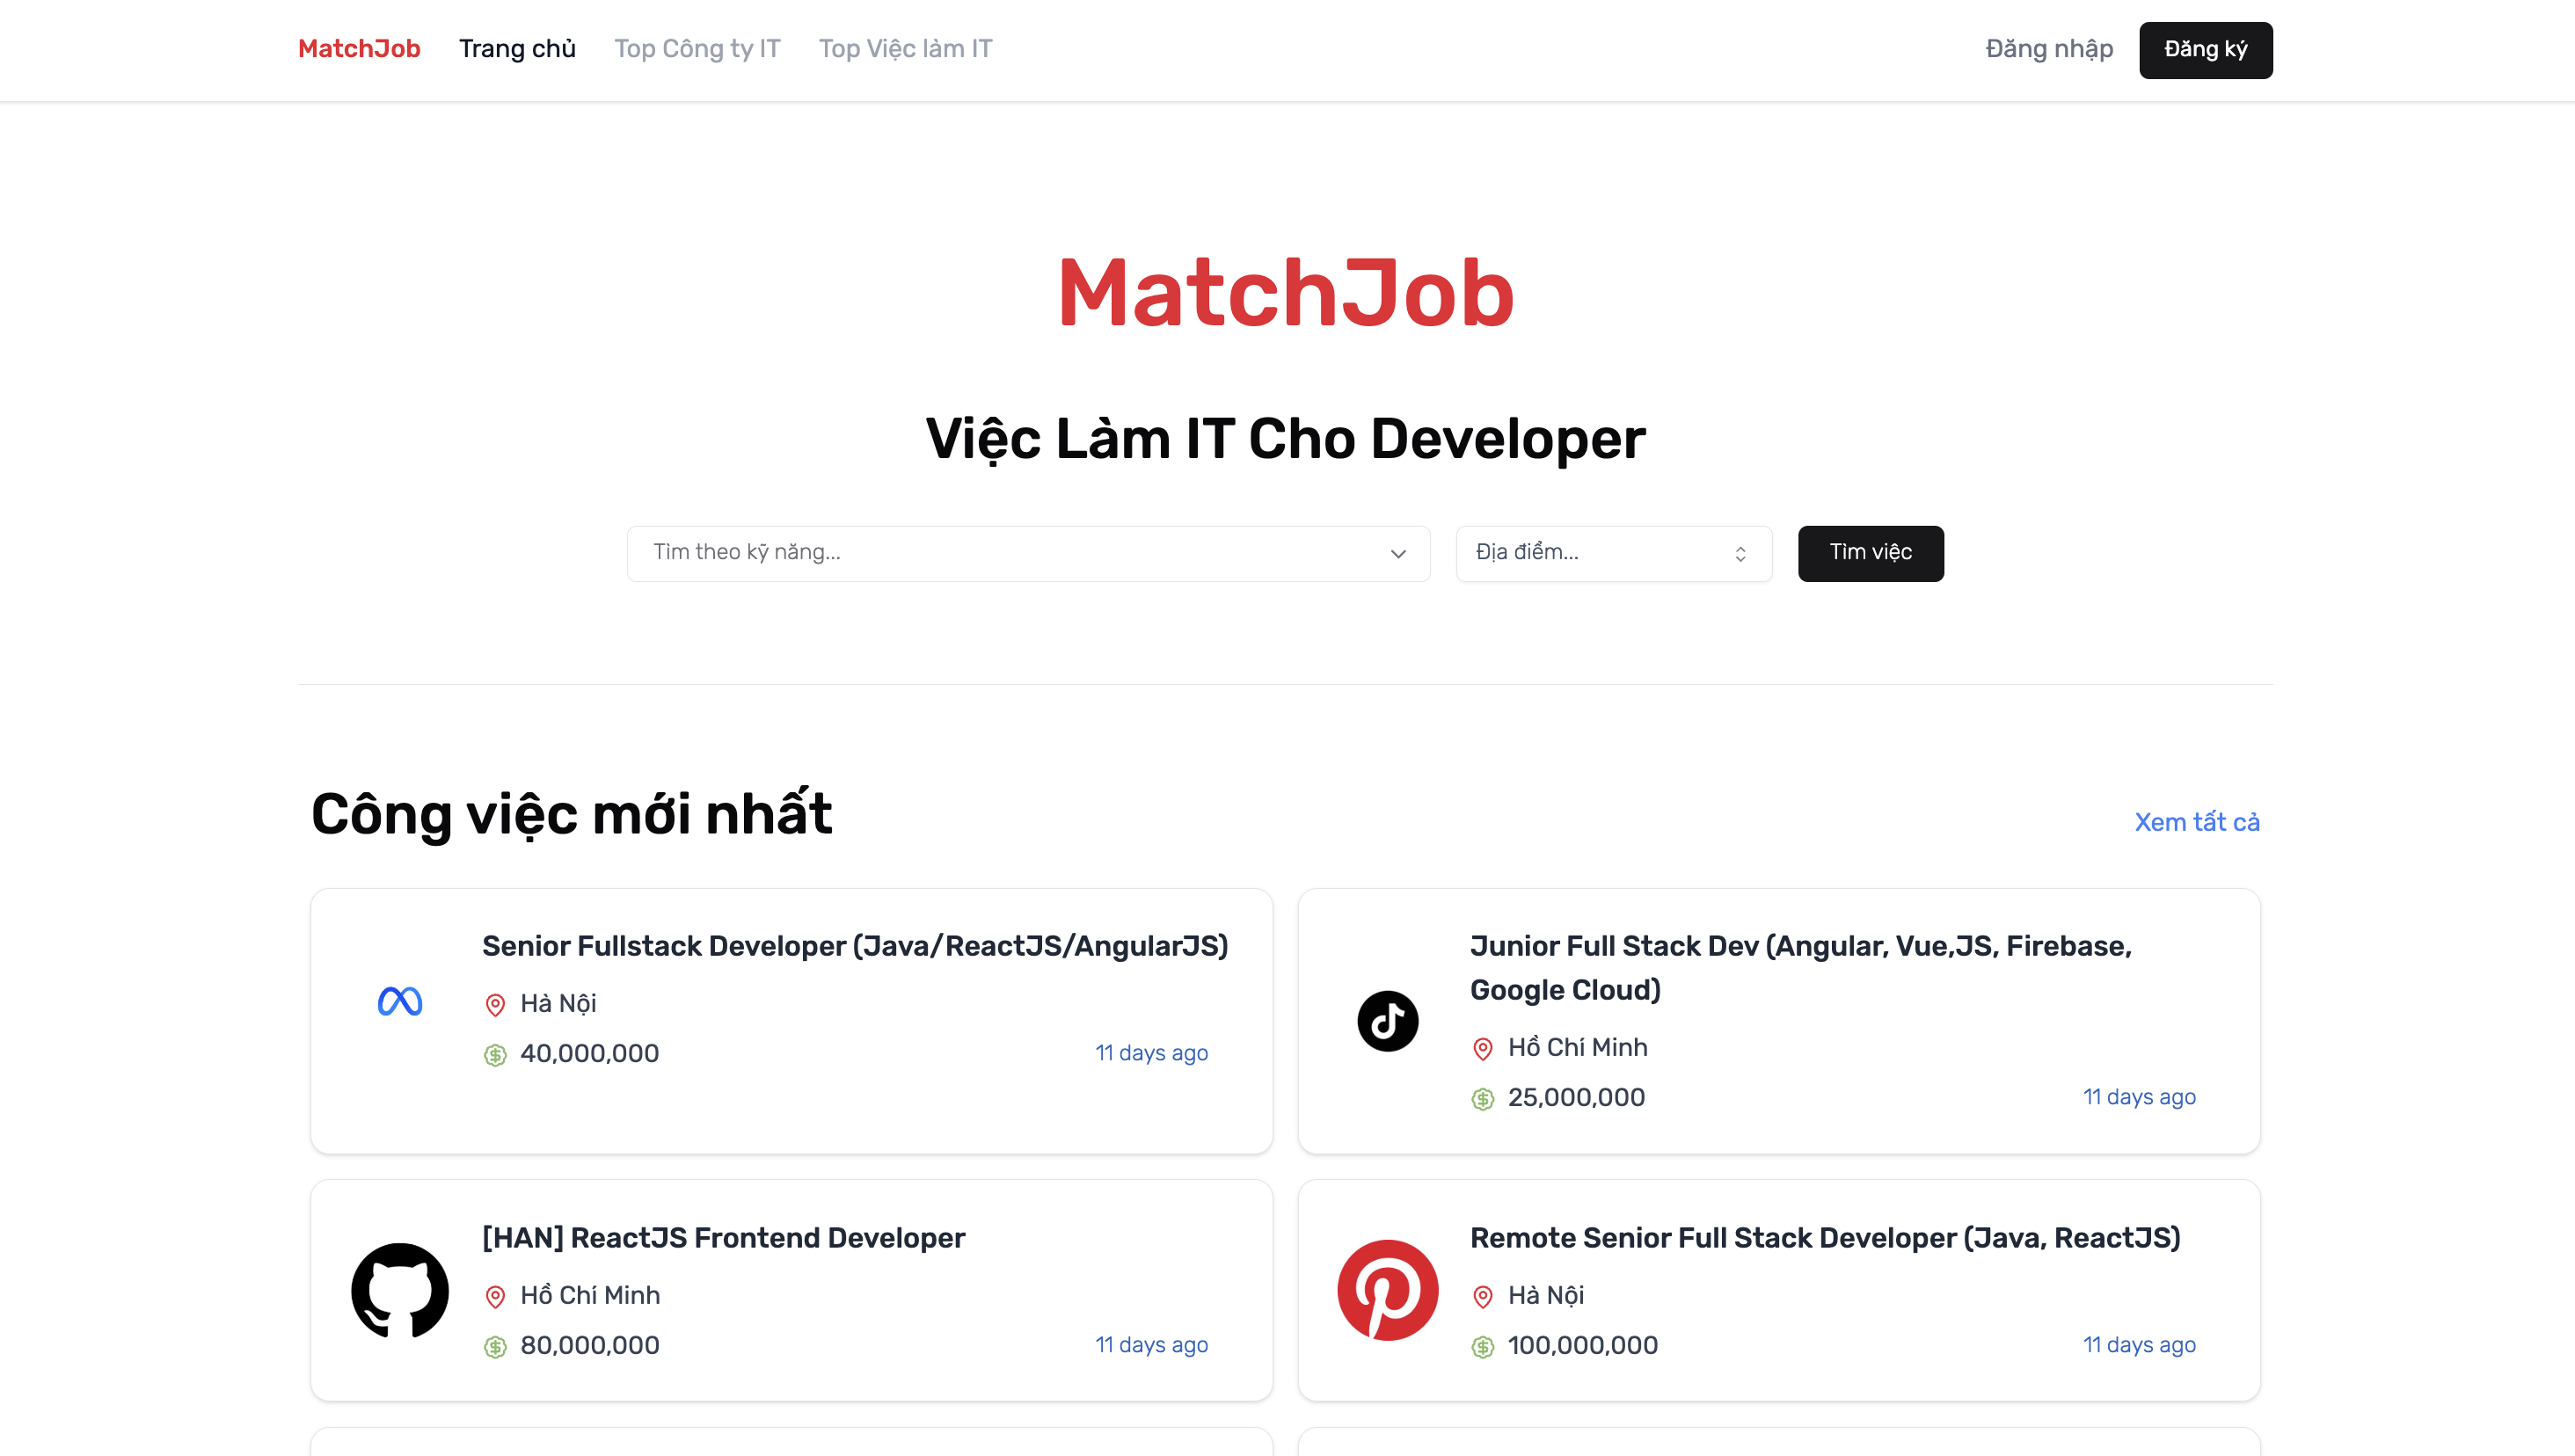
\includegraphics[width=\linewidth]{DBMS-Application/Images/user-screen-job.png}
    \caption{Trang chủ - Danh sách công việc đang tuyển dụng}
    \label{fig:homepage-job}
\end{figure}

Truy vấn sử dụng: \textbf{Query with composite condition}
\begin{lstlisting}
async findAll(current: number, pageSize: number, qs: string) {
    // Loc ra dieu kien filter va sort tu query parameters
    const { filter } = aqp(qs);

    // Truy van: Danh sach cong viec thoa man dieu kien filter
    const jobs = await this.db
      .collection('jobs')
      .find(filter)
      .skip((current - 1) * pageSize)
      .limit(pageSize)
      .toArray();

    // Tra ve response cho Frontend
    return jobs;
}
\end{lstlisting}

Giải thích:

\begin{enumerate}
    \item Frontend sẽ tự động gửi yêu cầu đến Backend thông qua API:
    \begin{lstlisting}[numbers=none]
GET /api/jobs?current=0&pageSize=6
    \end{lstlisting}
    
    \item Backend sẽ nhận được query parameters (\texttt{current} và \texttt{pageSize}) từ Frontend và thực hiện truy vấn CSDL với filter và phân trang:
    \begin{itemize}
        \item Sử dụng \texttt{find()} để lọc dữ liệu theo điều kiện \texttt{filter} (trong trường hợp này, \texttt{filter} là object rỗng (\texttt{\{\}}) nên sẽ trả về tất cả các công việc có trong hệ thống)
        \item Sử dụng \texttt{skip()} để bỏ qua các bản ghi không cần thiết
        \item Sử dụng \texttt{limit()} để giới hạn số lượng bản ghi trả về
    \end{itemize}

    \item Sau khi truy vấn được thực hiện thành công, Backend phản hồi danh sách các công việc cho Frontend để hiển thị lên giao diện người dùng
\end{enumerate}

Người dùng có thể tìm kiếm công việc bằng cách lọc theo \textbf{Địa điểm} và \textbf{Kỹ năng yêu cầu}. Ví dụ, tìm các công việc có yêu cầu kỹ năng \textbf{"React.JS"} và \textbf{"React Native"} tại \textbf{TP. Hồ Chí Minh}, hệ thống sẽ hiện lên một pop-up chứa các công việc thoả mãn.

\begin{figure}[H]
    \centering
    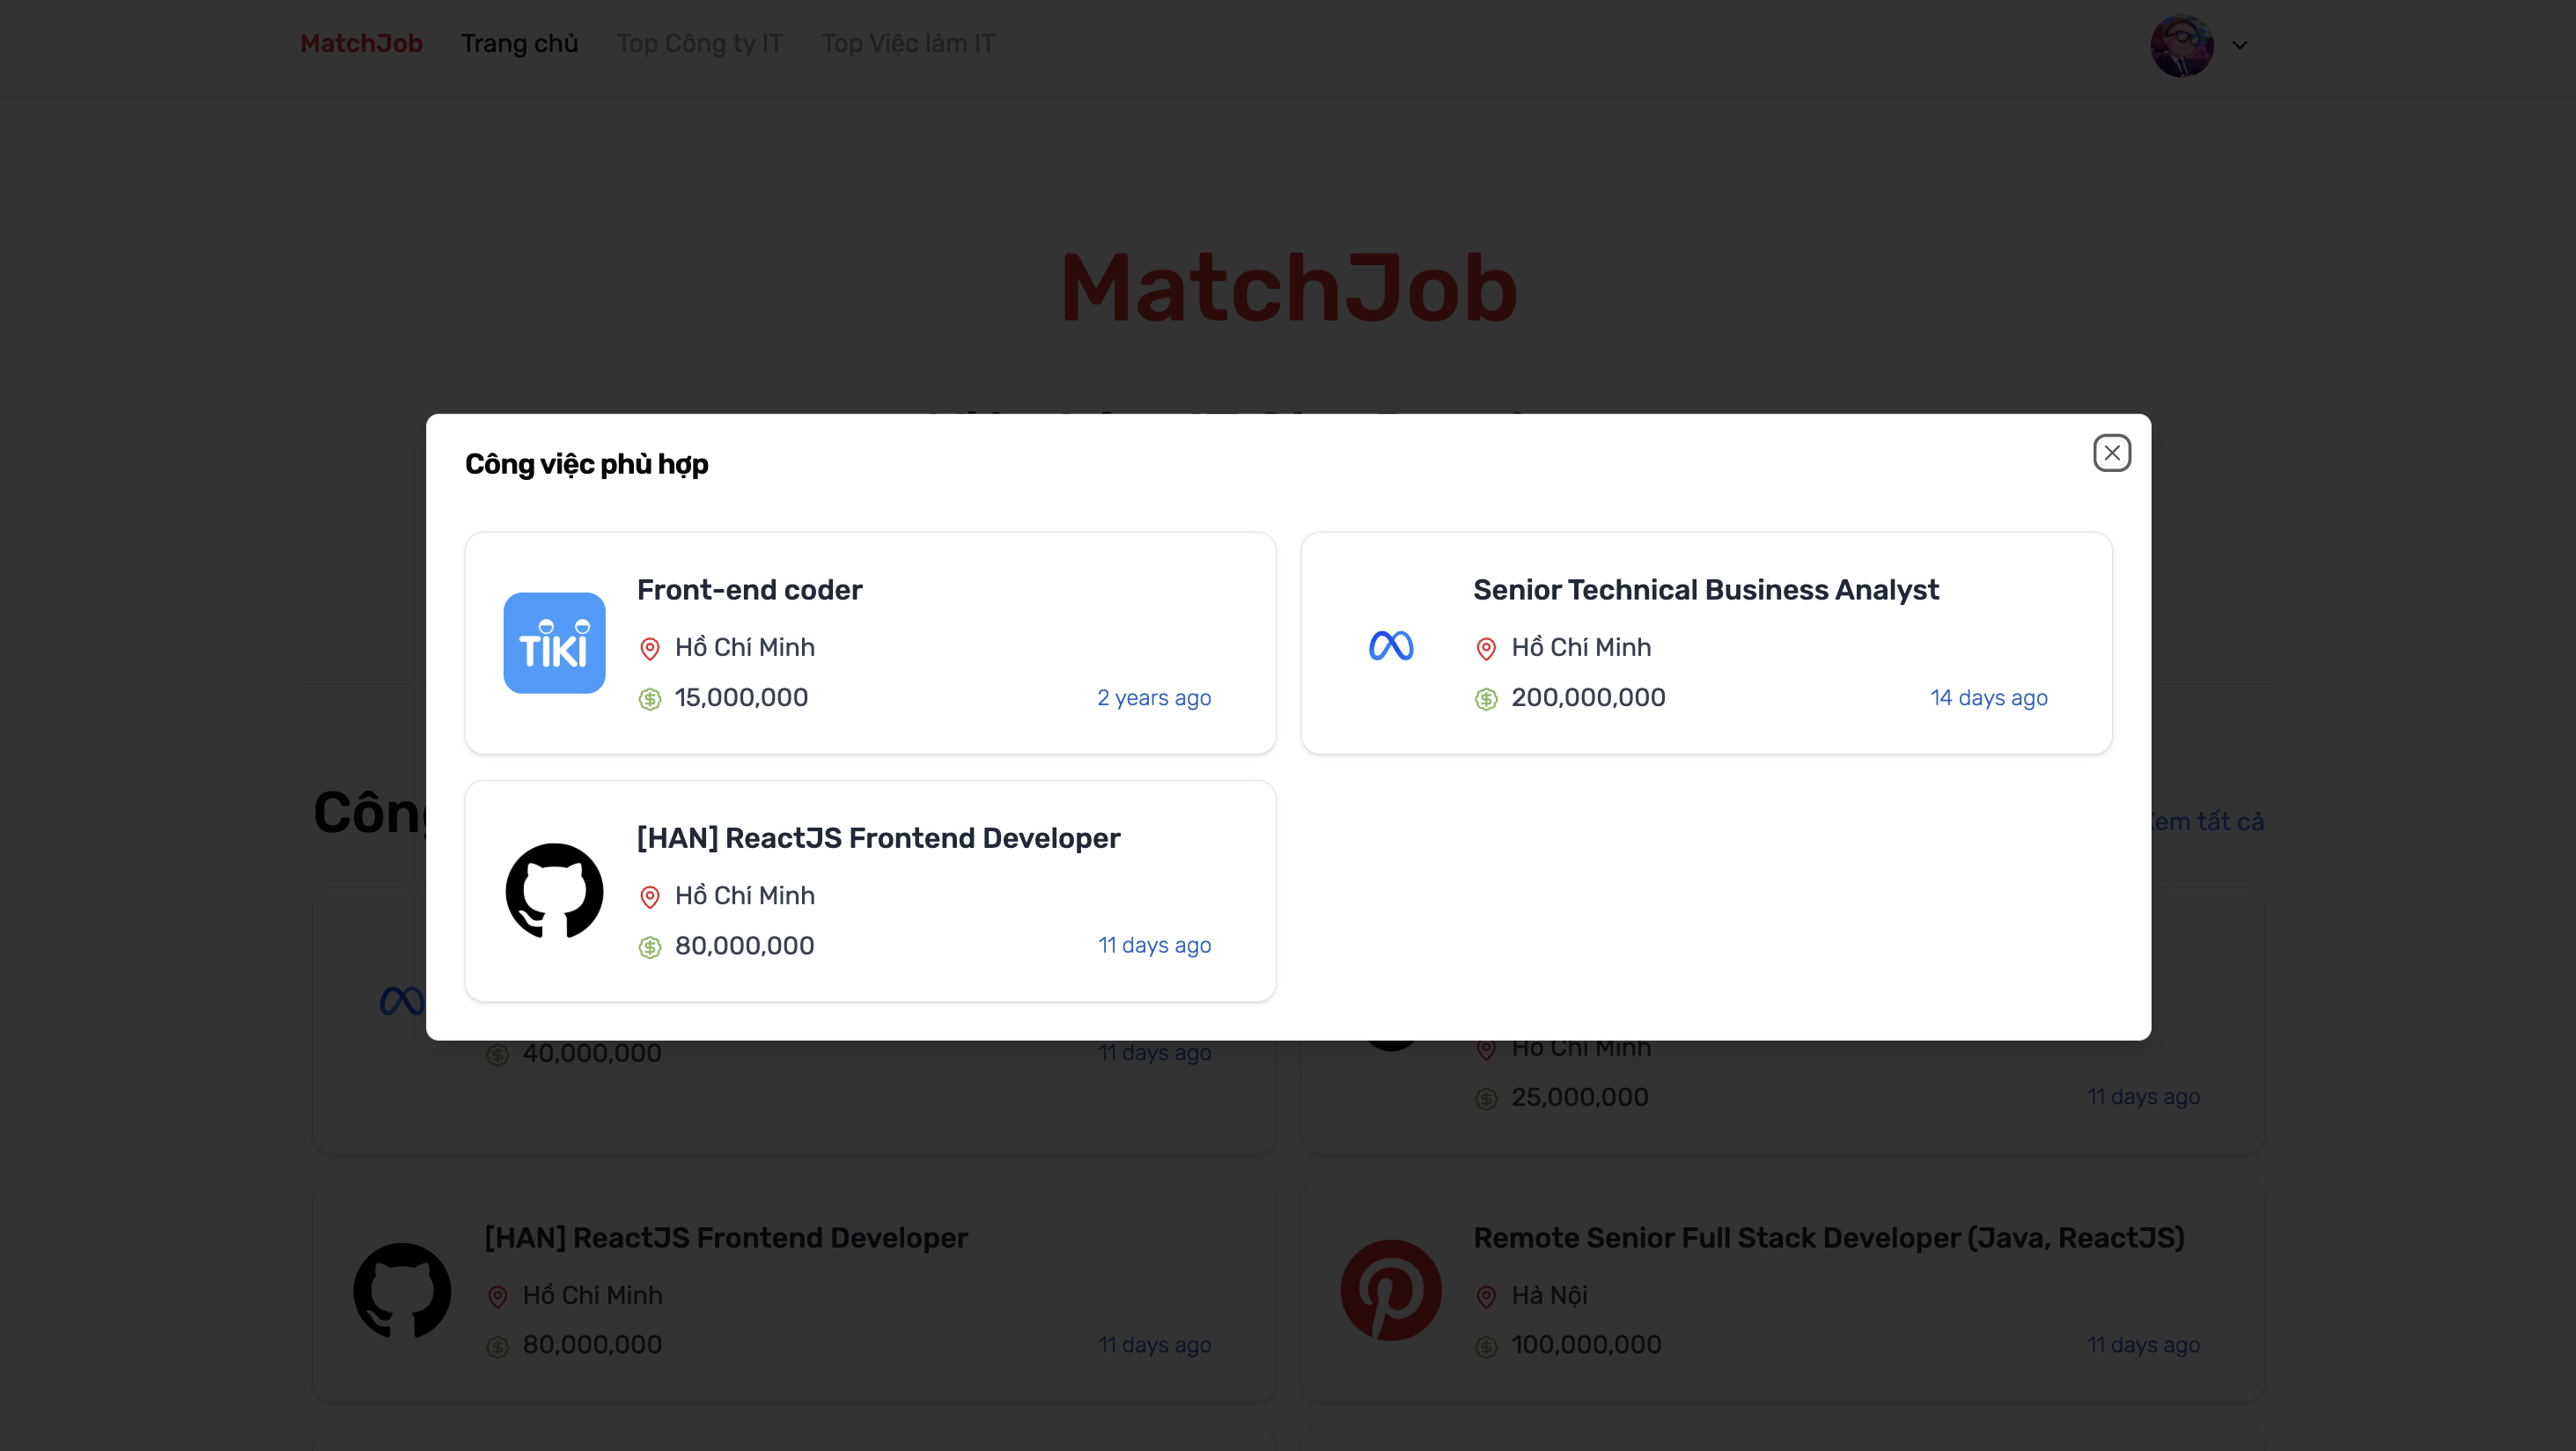
\includegraphics[width=\linewidth]{DBMS-Application/Images/modal-job-search.png}
    \caption{Trang chủ - Lọc công việc theo Địa điểm và Kỹ năng}
    \label{fig:homepage-job-search-filter}
\end{figure}

Truy vấn sử dụng: \textbf{Query with single/composite condition}

\begin{lstlisting}
async getJobsByLocationAndSkills(location: string, skills: string[]) {
    const query: { location?: string; skills?: { $in: string[] } } = {};

    if (location) query.location = location; 
    if (skills.length > 0) query.skills = { $in: skills }; 
    // query = { location: 'HOCHIMINH', skills: { $in: ['REACT.JS', 'REACT NATIVE'] } }

    // Truy van: Loc cac cong viec theo Ky nang va Dia diem
    return await this.db // Truy cap vao database he thong
    .collection('jobs')  // Truy cap vao collection 'jobs'
    .find(query)         // Loc theo dieu kien 'location' va 'skills' trong query
    .toArray();          // Chuyen ket qua ve dang mang
  }
\end{lstlisting}

Giải thích truy vấn:
\begin{itemize}
    \item Back-end nhận được yêu cầu từ Front-end, chứa 2 tham số \texttt{location} và \texttt{skills} trong query parameters và thực hiện xây dựng điều kiện lọc \texttt{query} với các giá trị đó
    
    Ví dụ: \texttt{ query = \{ location : ’HOCHIMINH’, skills : \{ \$in : [ ’REACT.JS’, ’REACT NATIVE’] \} \} }

    \item Sau đó, Back-end sẽ thực hiện truy vấn đến CSDL để lọc ra các công việc thoả mãn điều kiện vừa xây dựng được, và phản hồi về cho Front-end khi thành công
\end{itemize}

Người dùng cũng có thể xem được các công ty tuyển dụng hàng đầu cùng một số thông tin như: tên, logo công ty, số lượng công việc đang tuyển và thu thập cao nhất.

\begin{figure}[H]
    \centering
    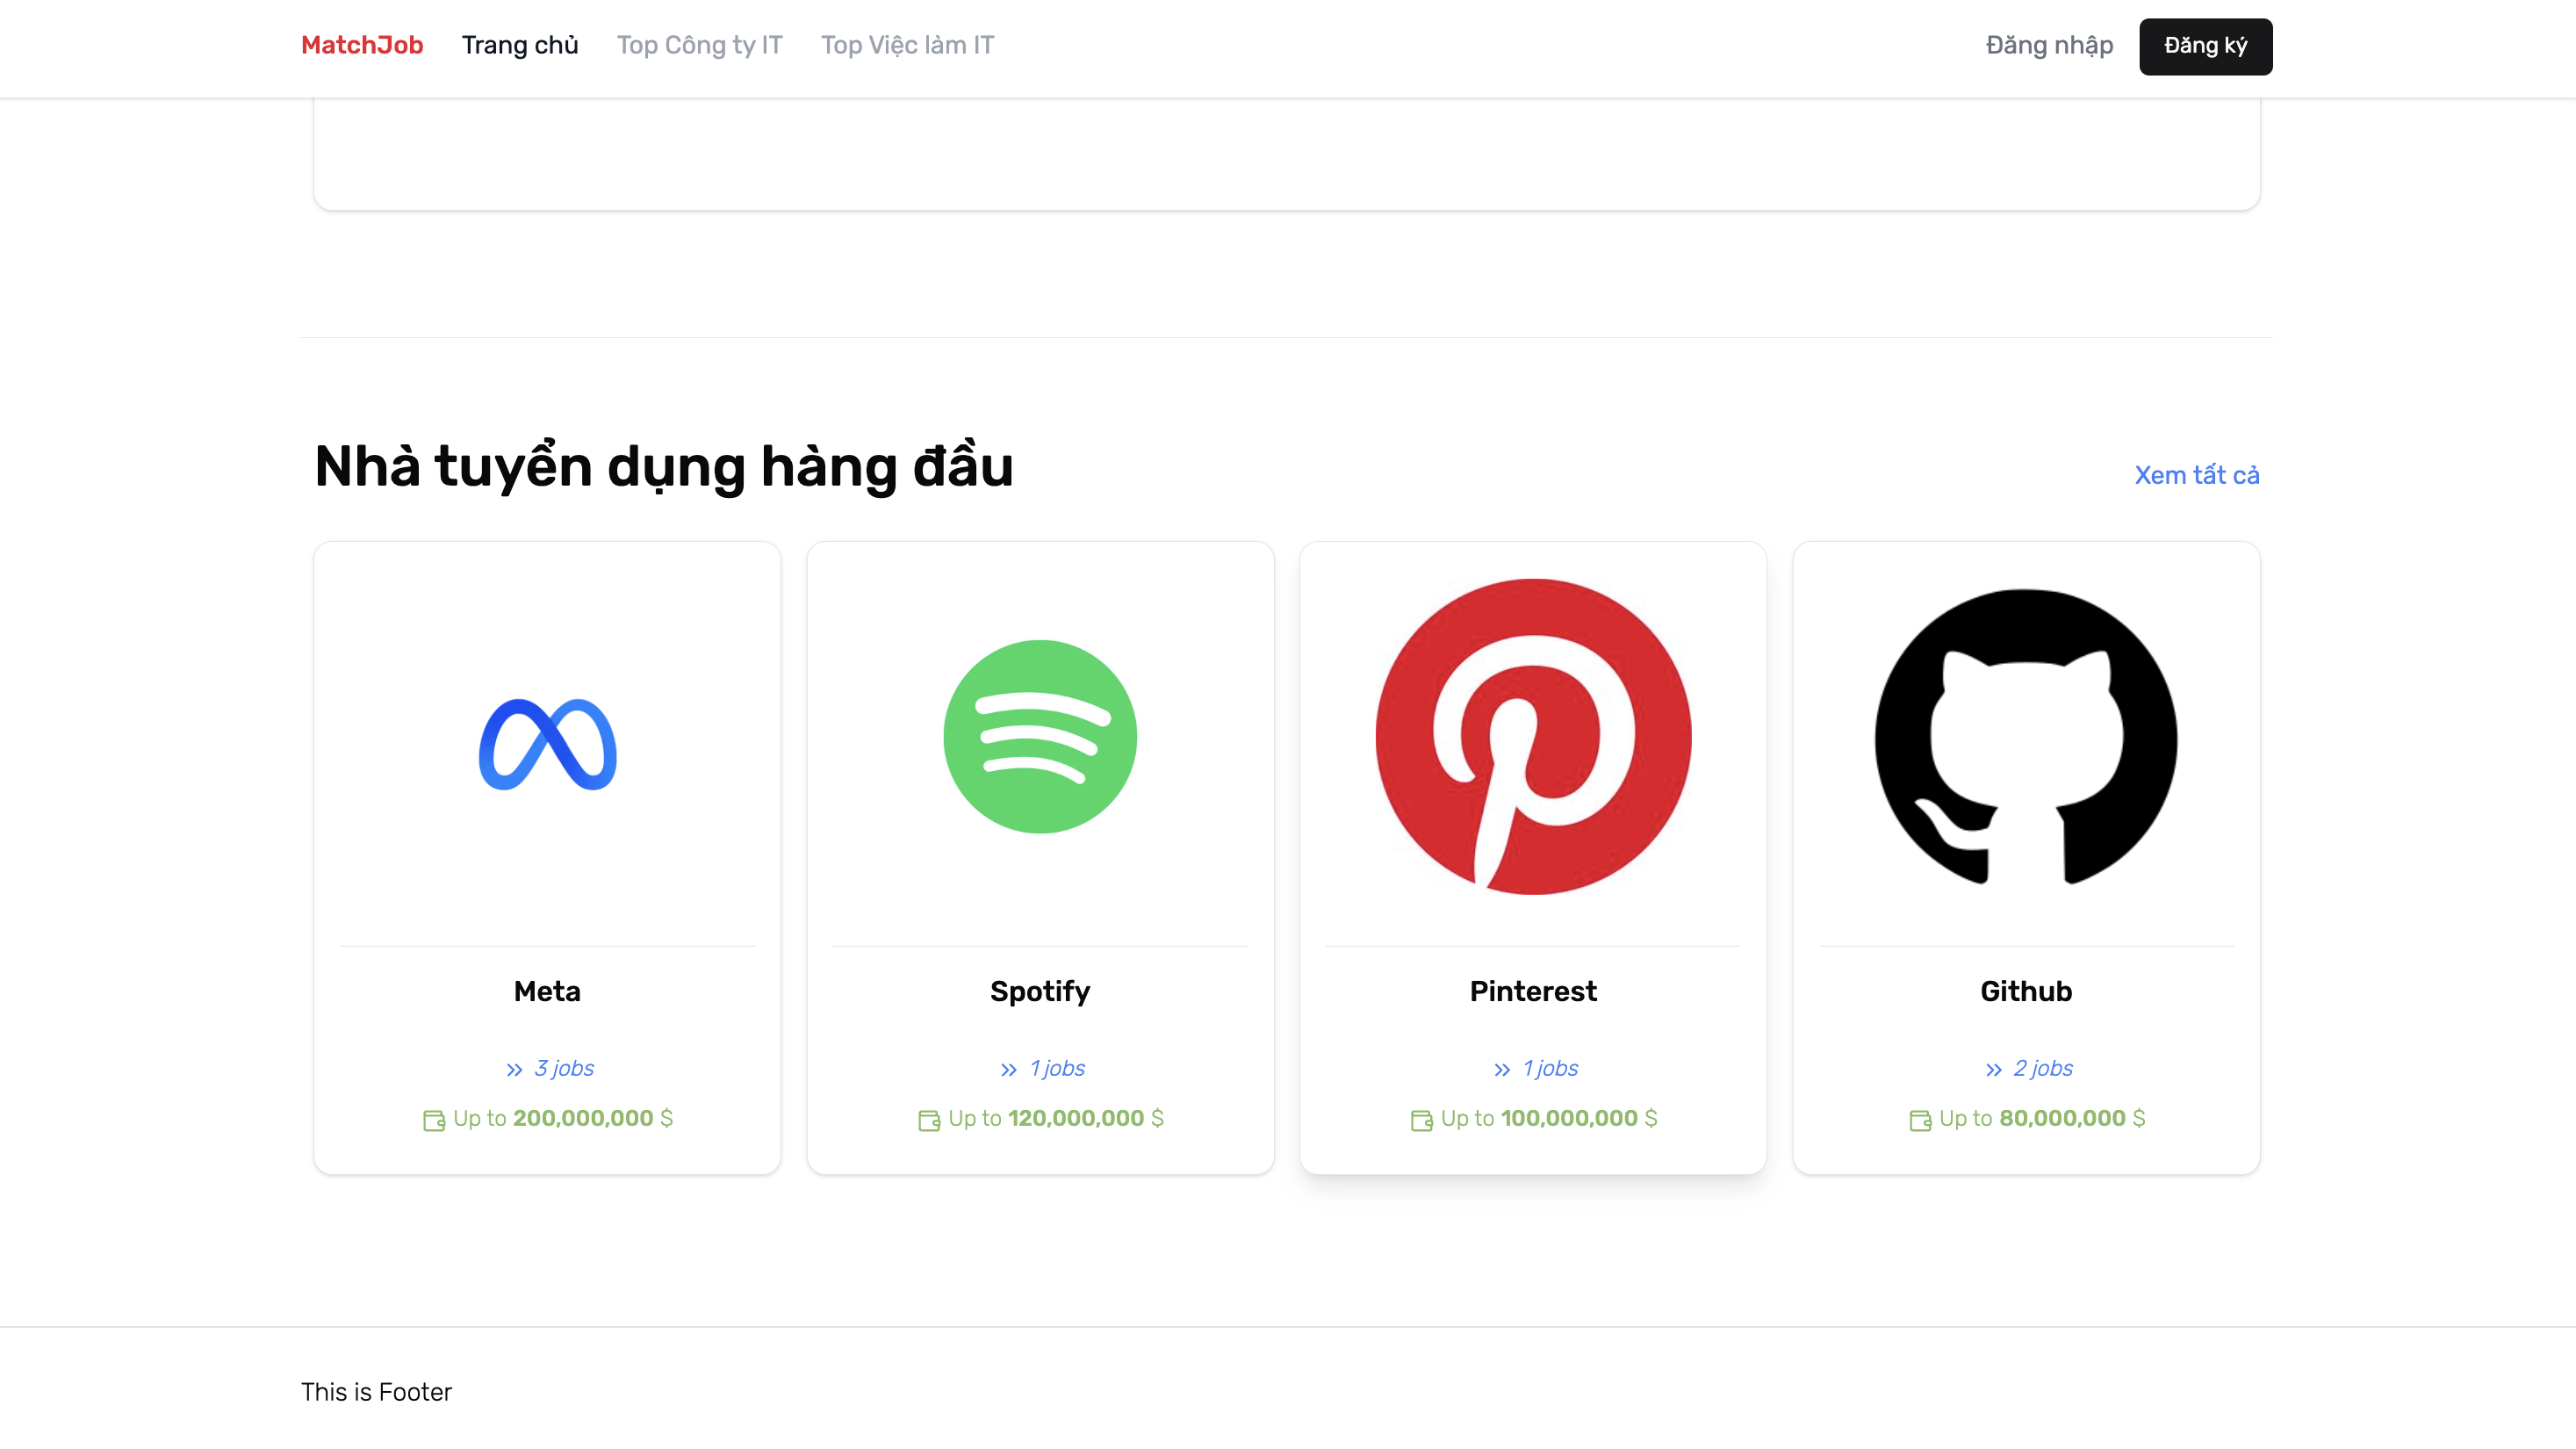
\includegraphics[width=\linewidth]{DBMS-Application/Images/user-screen-company.png}
    \caption{Trang chủ - Danh sách công ty tuyển dụng hàng đầu}
    \label{fig:homepage-company}
\end{figure}

Truy vấn sử dụng:
\begin{itemize}
    \item \textbf{Query with join}: Sử dụng và \texttt{\$lookup} để join collections \textbf{companies} với \textbf{jobs}
    \item \textbf{Query with aggregation functions}: Sử dụng \texttt{\$size}, \texttt{\$max}, \texttt{\$reduce} để tính toán số lượng công việc, mức lương cao nhất của công ty
\end{itemize}

\begin{lstlisting}
const pipeline = [
  { $match: filter },
  {
    $lookup: {
      from: 'jobs',
      let: { companyId: { $toString: '$_id' } },
      pipeline: [
        {
          $match: {
            $expr: {
              $eq: ['$company._id', '$$companyId'],
            },
          },
        },
      ],
      as: 'jobs',
    },
  },
  {
    $project: {
      _id: 1,
      name: 1,
      address: 1,
      description: 1,
      logo: 1,
      totalJobs: { $size: '$jobs' }, // Dem so luong cong viec
      maxSalary: { $max: '$jobs.salary' }, // Lay ra salary cao nhat
      maxSalaryJobId: {
        $reduce: {
          input: '$jobs',
          initialValue: null,
          in: {
            $cond: [
              { $eq: ['$$this.salary', { $max: '$jobs.salary' }] },
              '$$this._id',
              '$$value',
            ],
          },
        },
      },
    },
  },
  { $sort: { maxSalary: -1 } }, // Sap xep cong ty giam dan theo maxSalary
  { $skip: offset },
  { $limit: limit },
];

return await this.db
  .collection('companies')
  .aggregate(pipeline)
  .toArray();
\end{lstlisting}

Giải thích truy vấn: 
\begin{itemize}
    \item \texttt{\$match}: Lọc các công ty thỏa mãn điều kiện.
    \item \texttt{\$lookup}: Join collection \textbf{companies} (\texttt{\_id}) collection \textbf{jobs} (\texttt{companyId}) để lấy các công việc ứng với từng công ty
    \item \texttt{\$project}: Lọc ra các trường trong collection \textbf{companies} như \texttt{\_id}, \texttt{name}, \texttt{address}, \texttt{logo} và Tính toán các thông tin thống kê như số lượng công việc (\texttt{totalJobs}), lương cao nhất (\texttt{maxSalary}) và ID công việc có lương cao nhất (\texttt{maxSalaryJobId}) của từng công ty
    \item \texttt{\$sort}: Sắp xếp các công ty giảm dần theo lương cao nhất (\texttt{maxSalary})
    \item \texttt{\$skip} và \texttt{\$limit}: Phân trang kết quả
\end{itemize}

Bên cạnh đó, người dùng có thể xem nhanh thông tin các công việc đang tuyển dụng của một công ty cụ thể, thông qua các thẻ công ty được hiển thị:

\begin{figure}[H]
    \centering
    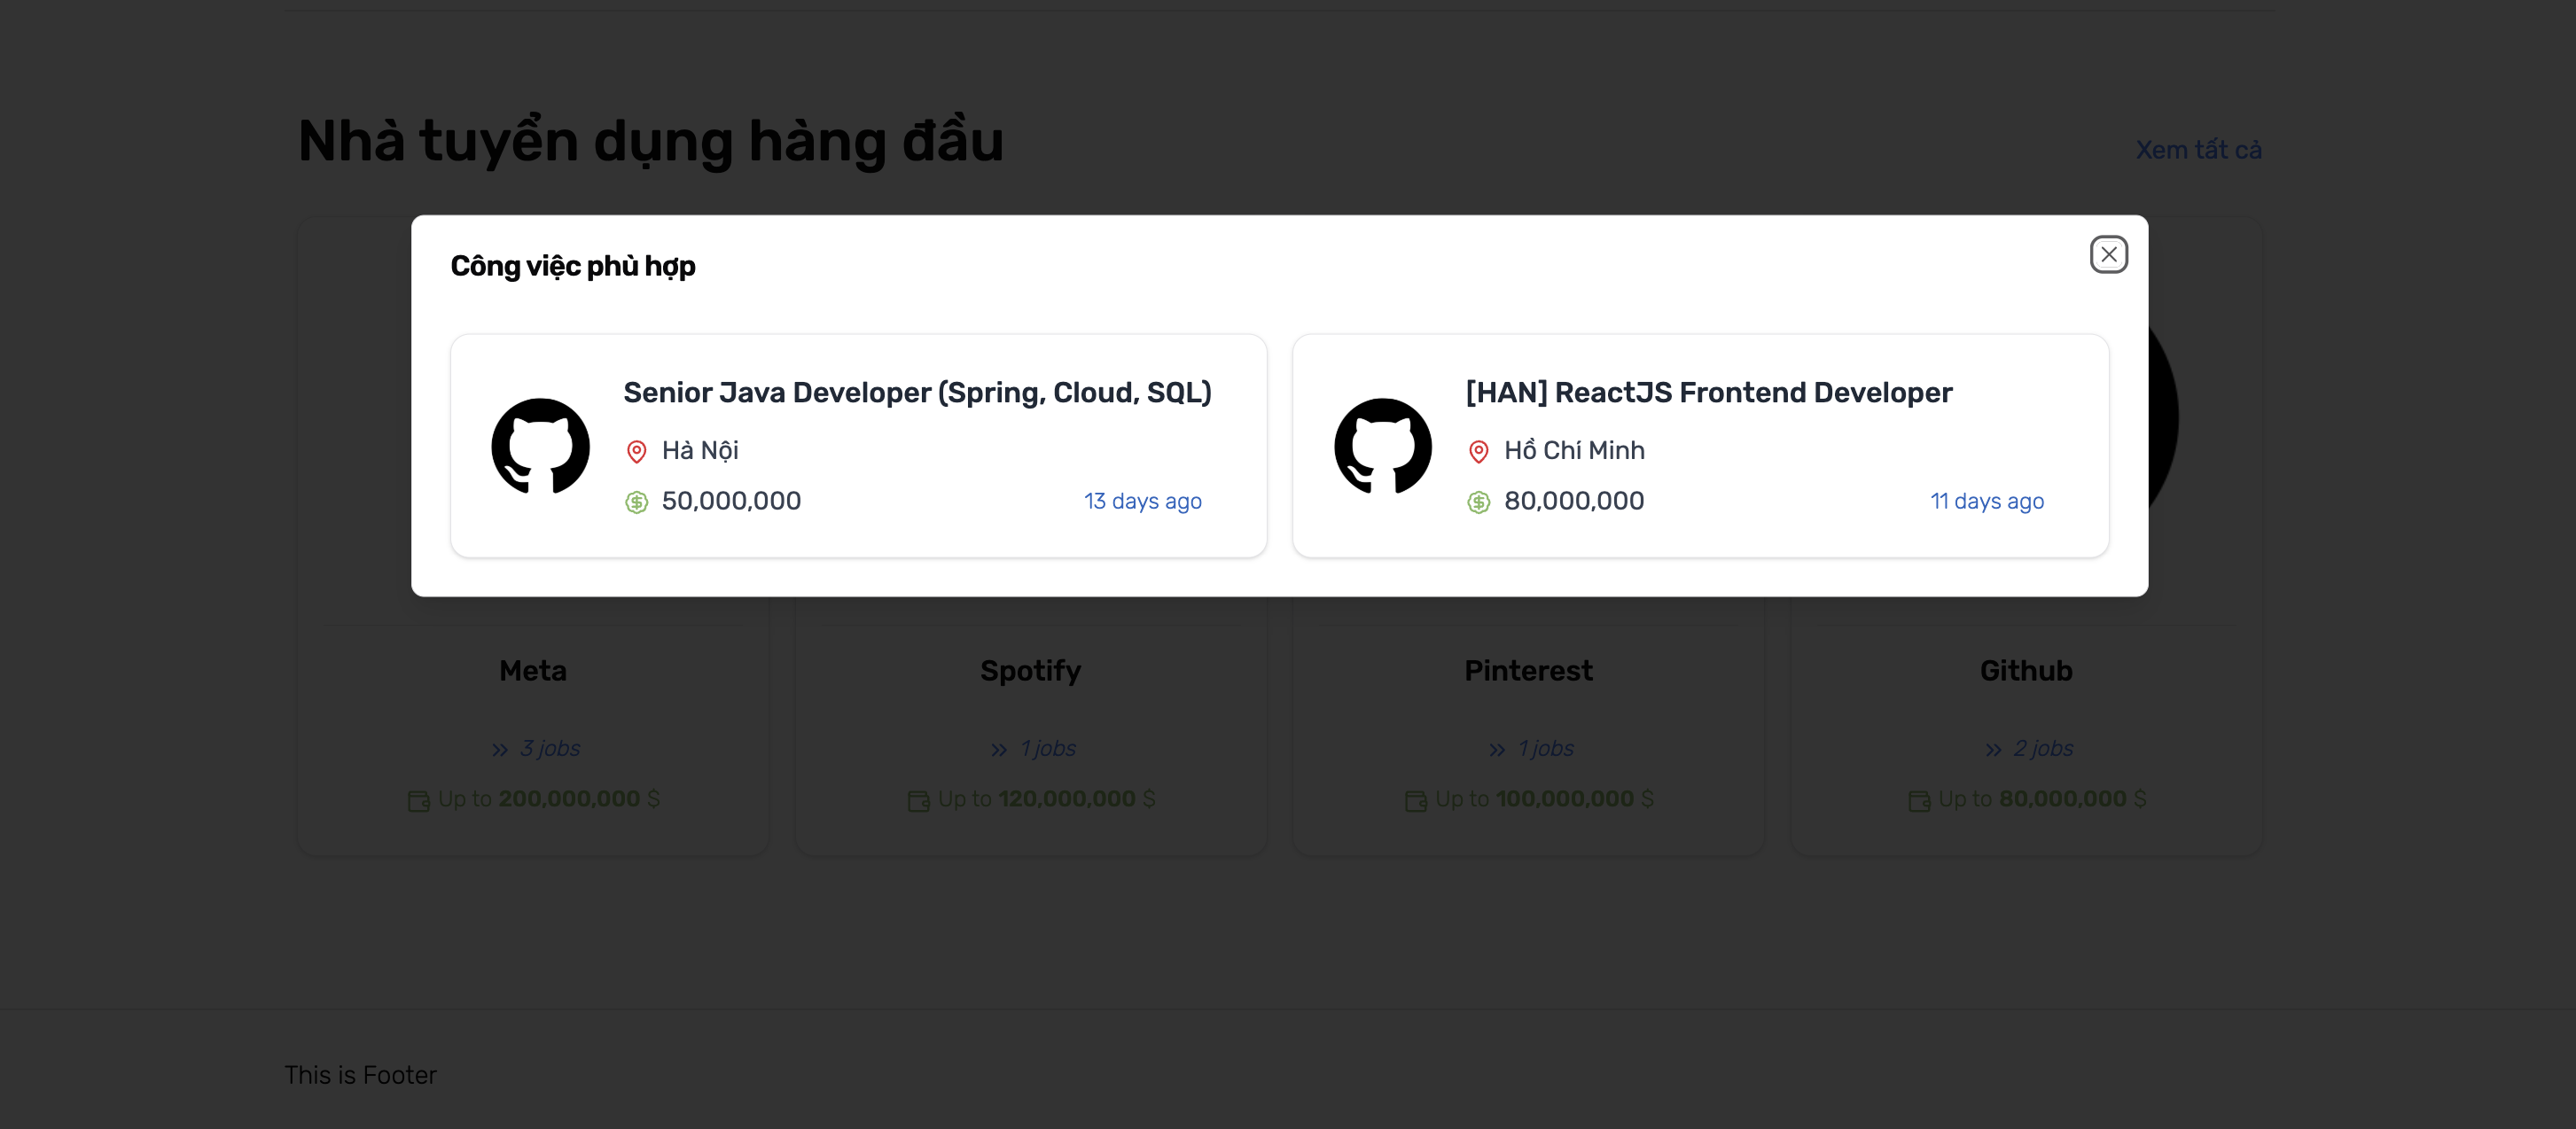
\includegraphics[width=\linewidth]{DBMS-Application/Images/modal-job-company.png}
    \caption{Trang chủ - Lọc ra các công việc thuộc một công ty cụ thể}
    \label{fig:homepage-job-company}
\end{figure}

Truy vấn sử dụng:
\begin{itemize}
    \item \textbf{Query with single condition}: Lọc document cụ thể từ collection \textbf{companies} dựa trên \texttt{\_id}

    \item \textbf{Query with join}: Thực hiện join giữa collection \textbf{companies} và \textbf{jobs} để lấy công việc liên quan
\end{itemize}

\begin{lstlisting}
const pipeline = [
  {
    $match: { _id: new ObjectId(companyId) }, // Loc ra cong ty co _id = companyId duoc truyen vao
  },
  {
    $lookup: {
      from: 'jobs', // Join collection 'companies' voi collection 'jobs'
      let: { companyId: { $toString: '$_id' } },
      pipeline: [
        {
          $match: {
            $expr: { $eq: ['$company._id', '$$companyId'] },
          },
        },
      ],
      as: 'jobs', // Luu ket qua vao field 'jobs' cho tung cong ty
    },
  },
  {
    $project: { // Loc ra cac field can thiet
      _id: 1,
      name: 1,
      address: 1,
      description: 1,
      logo: 1,
      jobs: 1,
    },
  },
];

return await this.db
  .collection('companies')
  .aggregate(pipeline)
  .toArray();
\end{lstlisting}

Giải thích truy vấn:
\begin{itemize}
    \item \texttt{\$match}: Lọc công ty cụ thể từ collection companies dựa trên \texttt{\_id} được truyền vào (\texttt{companyId}).
    
    \item \texttt{\$lookup}: Join collection \textbf{companies} với collection \textbf{jobs} để tìm tất cả các công việc thuộc công ty đó, bằng cách so sánh \texttt{\_id} của công ty trong \textbf{companies} với \texttt{company.\_id} trong \textbf{jobs} và lưu danh sách công việc vào trường \textbf{jobs}.


    \item \texttt{\$project}: Chọn các trường cần trả về gồm \texttt{\_id}, \texttt{name}, \texttt{address}, \texttt{description}, \texttt{logo}, và \texttt{jobs}.
\end{itemize}

Cuối cùng, người dùng có thể xem thống kê các kỹ năng có nhu cầu tuyển dụng nhiều, được thu thập từ các công việc đang được tuyển dụng:

\begin{figure}[H]
    \centering
    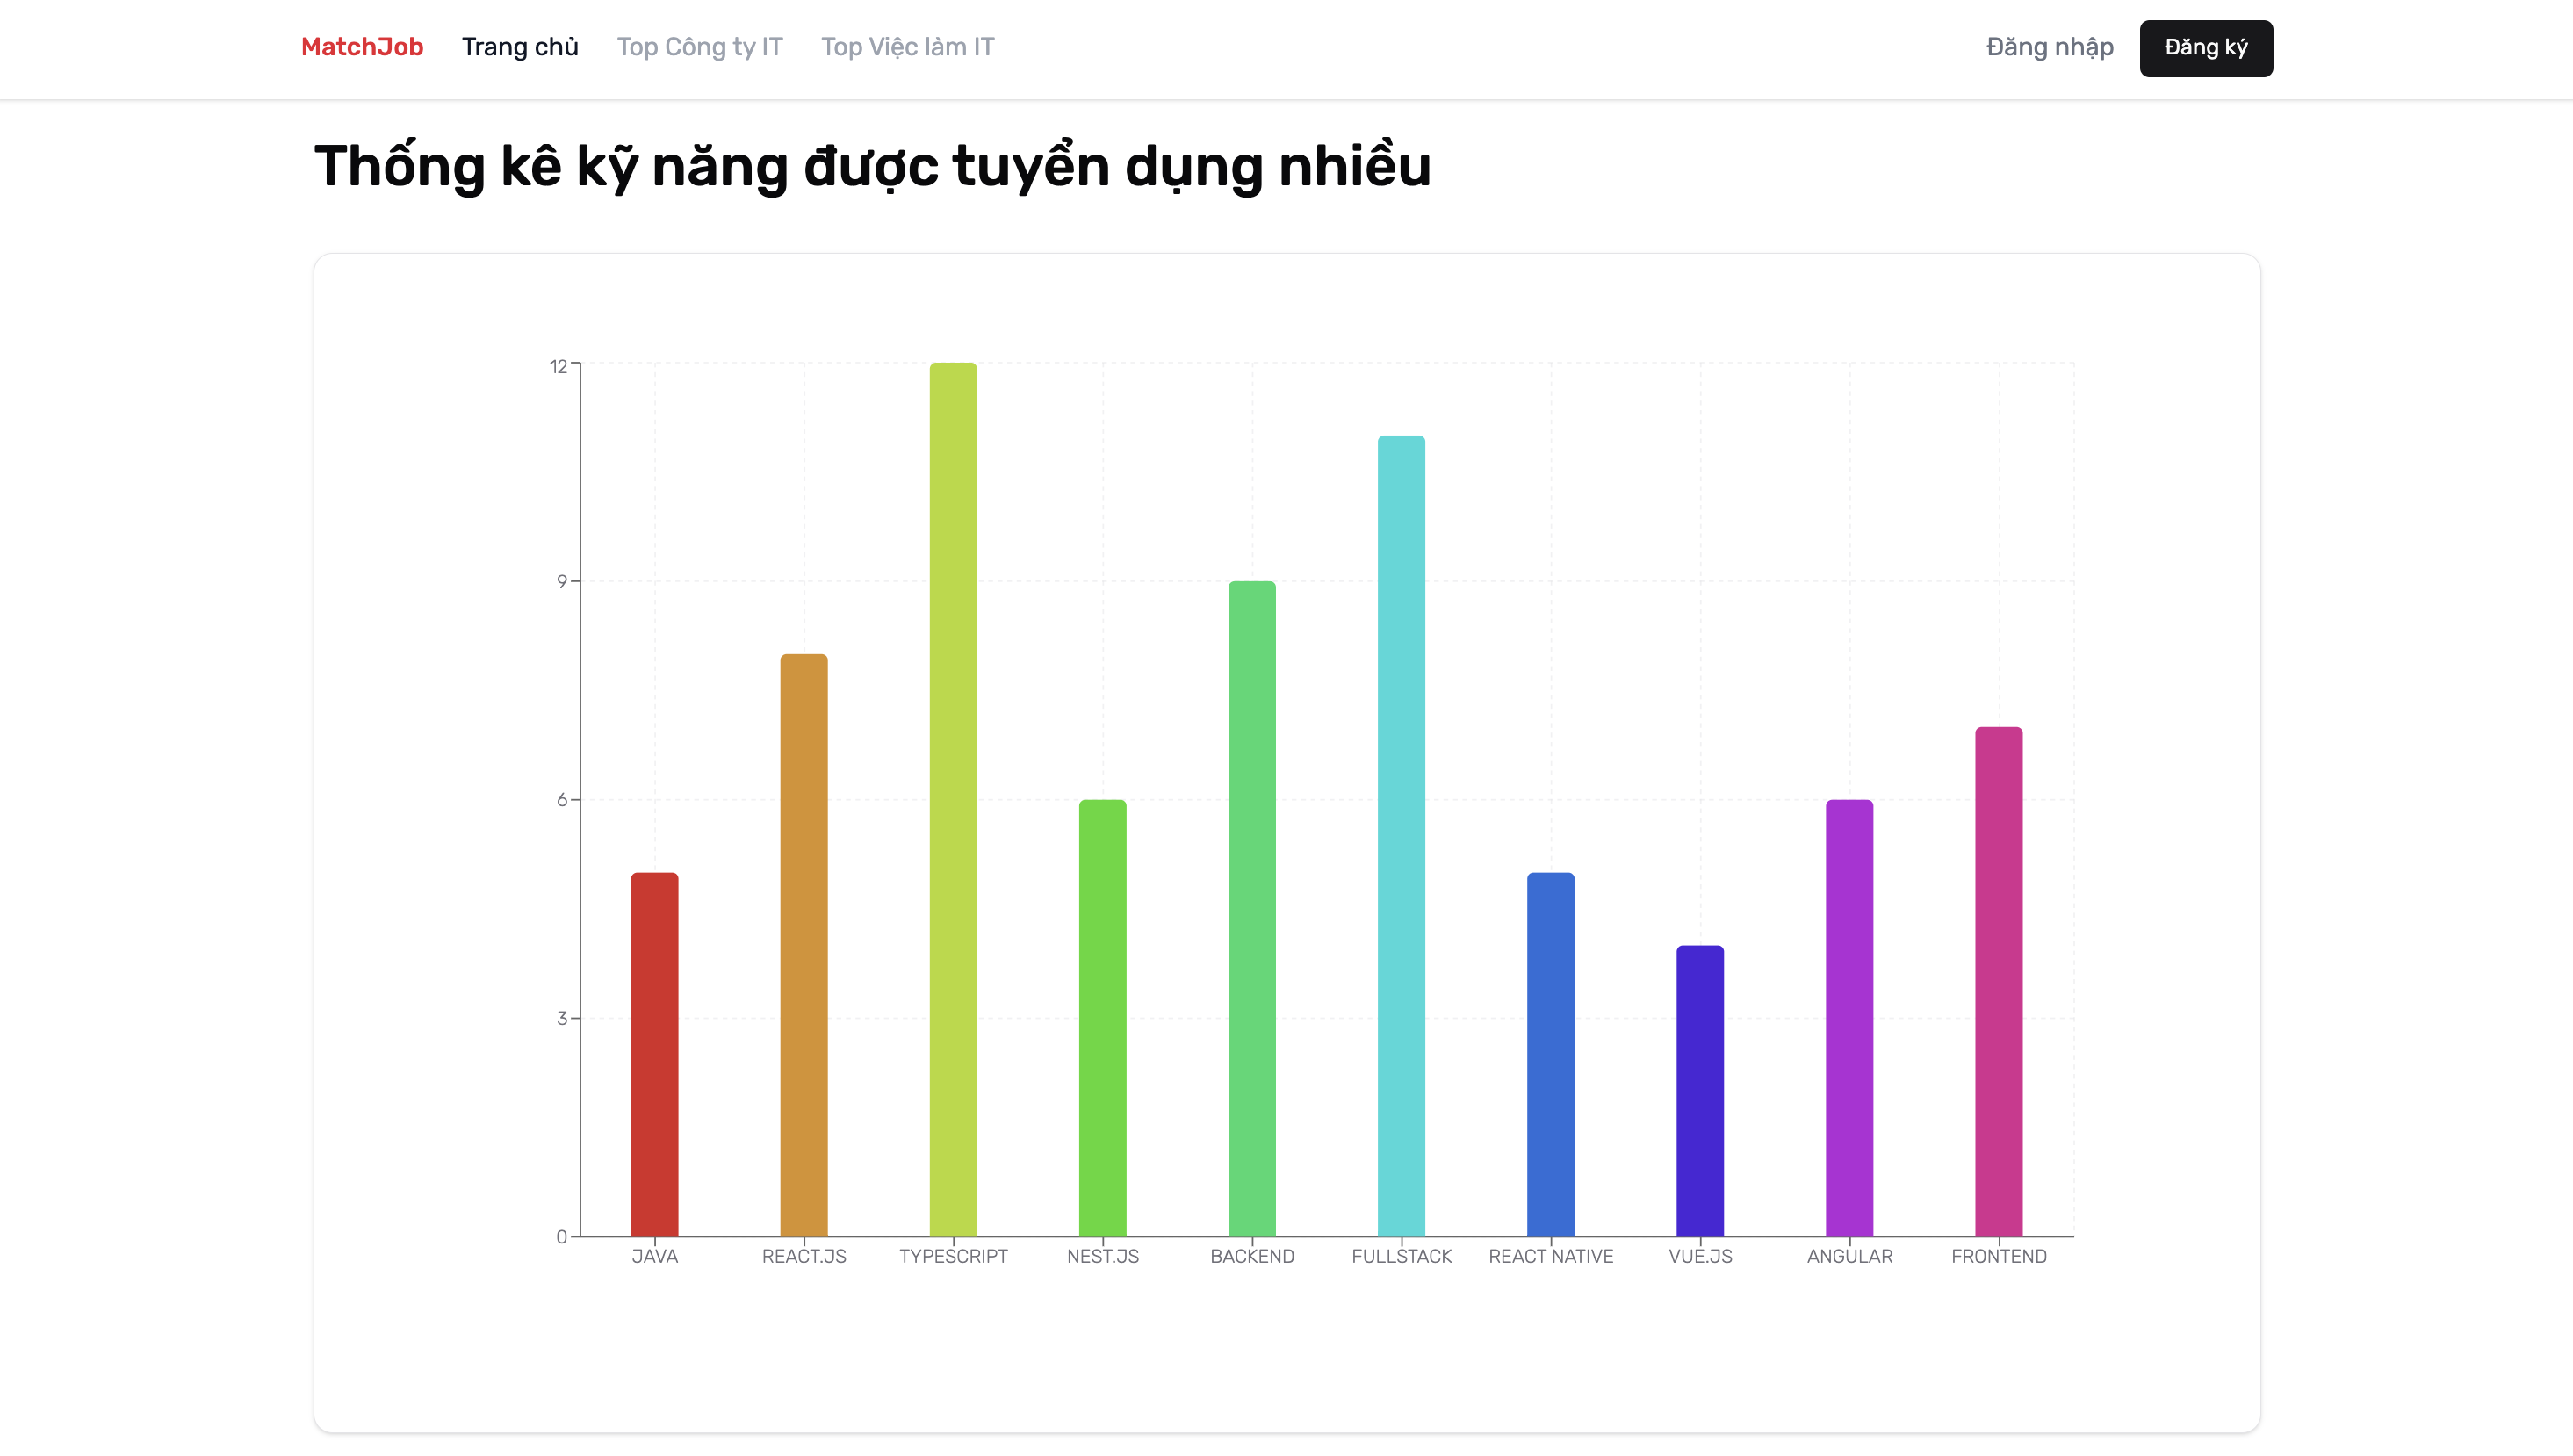
\includegraphics[width=\linewidth]{DBMS-Application/Images/user-screen-skill-stats.png}
    \caption{Trang chủ - Thống kê kỹ năng được tuyển dụng nhiều}
    \label{fig:enter-label}
\end{figure}

Truy vấn sử dụng: \textbf{Query with aggregation functions} - Sử dụng \texttt{\$sum} để tính tổng số công việc yêu cầu từng kỹ năng.

\begin{lstlisting}
const pipeline = [
  { $unwind: '$skills' },
  { $group: { _id: '$skills', total: { $sum: 1 } } },
  { $project: { skill: '$_id', total: 1, _id: 0 } },
];

return await this.db
  .collection('jobs')
  .aggregate(pipeline)
  .toArray();
\end{lstlisting}

Giải thích truy vấn:
\begin{itemize}
    \item \texttt{\$unwind}: Tách từng phần tử trong mảng skills của mỗi công việc thành các document riêng lẻ.
    \item \texttt{\$group}: Nhóm các document theo kỹ năng (skills) và đếm số lượng công việc yêu cầu kỹ năng đó bằng cách cộng dồn (\$sum: 1).
    \item \texttt{\$project}: Chọn các trường cần trả về, đổi tên \_id thành skill và bỏ trường \_id trong kết quả.
\end{itemize}

% \subsubsection{Giao diện người dùng - Danh sách/Chi tiết công ty}

Khi truy cập vào trang danh sách công ty, Front-end sẽ tự động fetch dữ liệu từ Backend thông qua một API tương tự như ở trang chủ: thực hiện phân trang để lấy lần lượt các công ty trong cơ sở dữ liệu dựa trên tham số \texttt{current} và \texttt{pageSize}.

\begin{figure}[H]
    \centering
    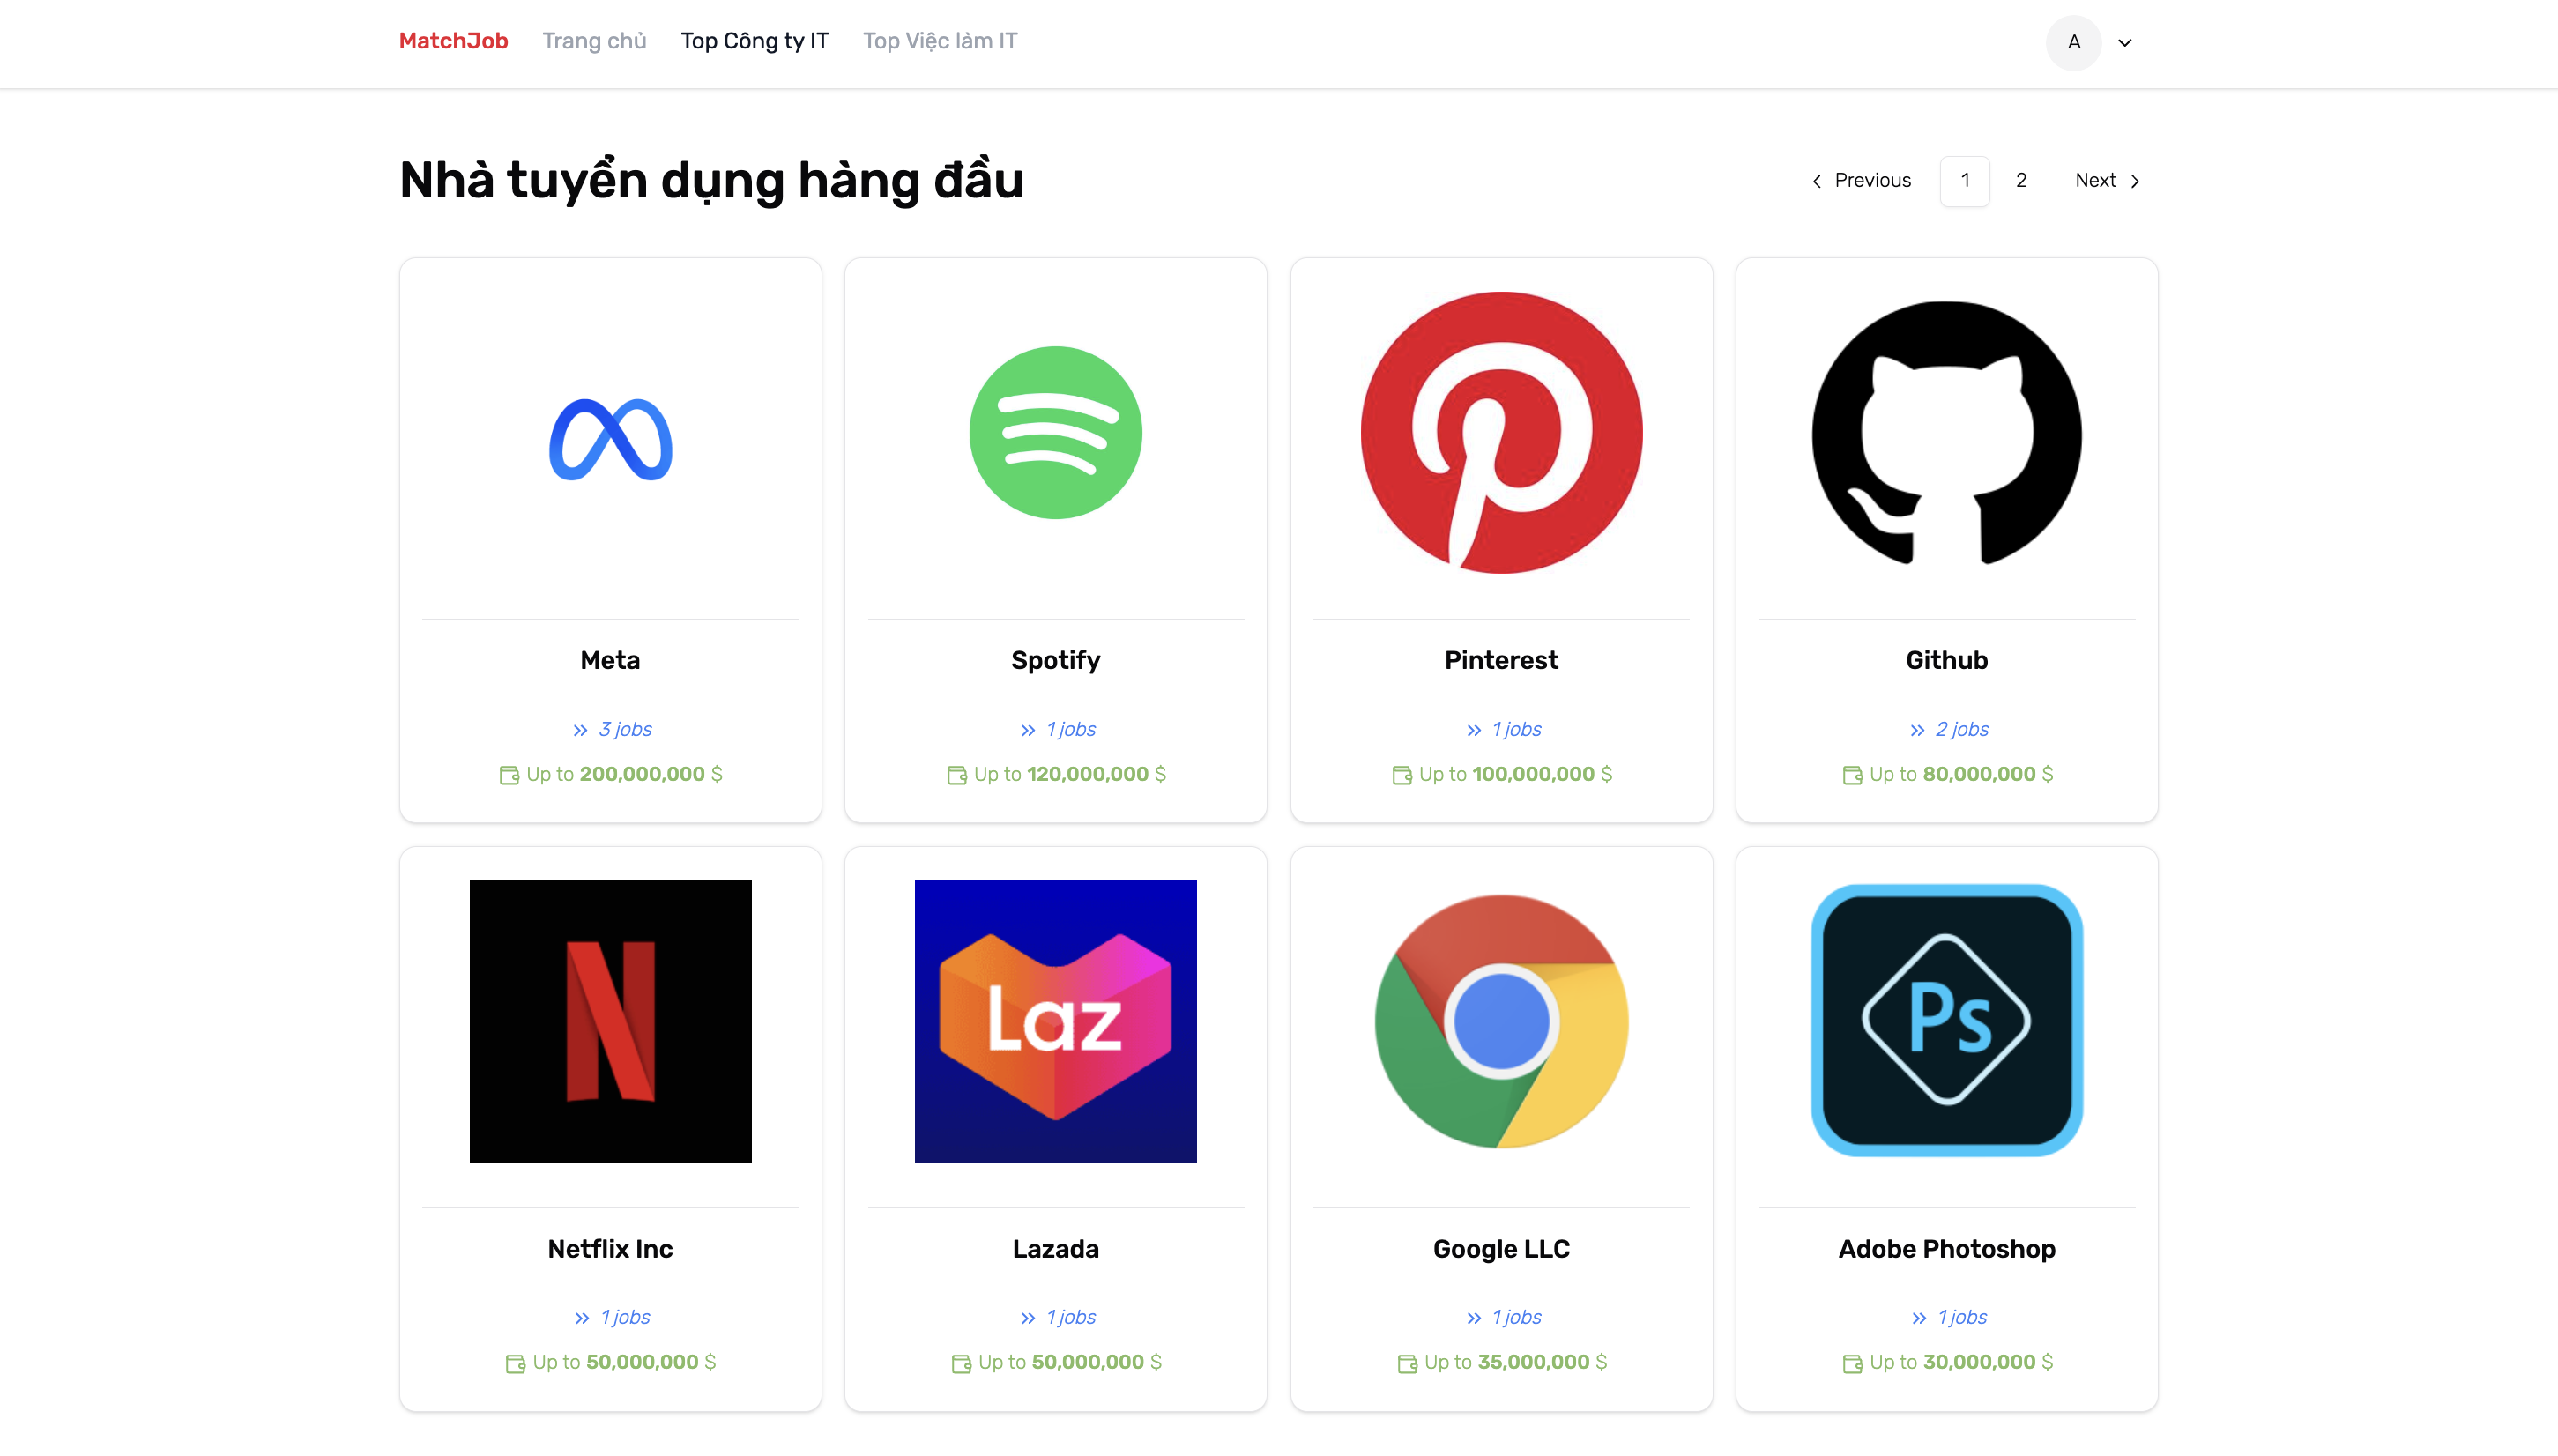
\includegraphics[width=\linewidth]{DBMS-Application/Images/list-company.png}
    \caption{Danh sách công ty}
    \label{fig:enter-label}
\end{figure}

Khi người dùng chọn 1 công ty trong danh sách, Front-end sẽ gửi yêu cầu đến API để lấy thông tin chi tiết của công ty đó và hiển thị lên giao diện người dùng:

\begin{figure}[H]
    \centering
    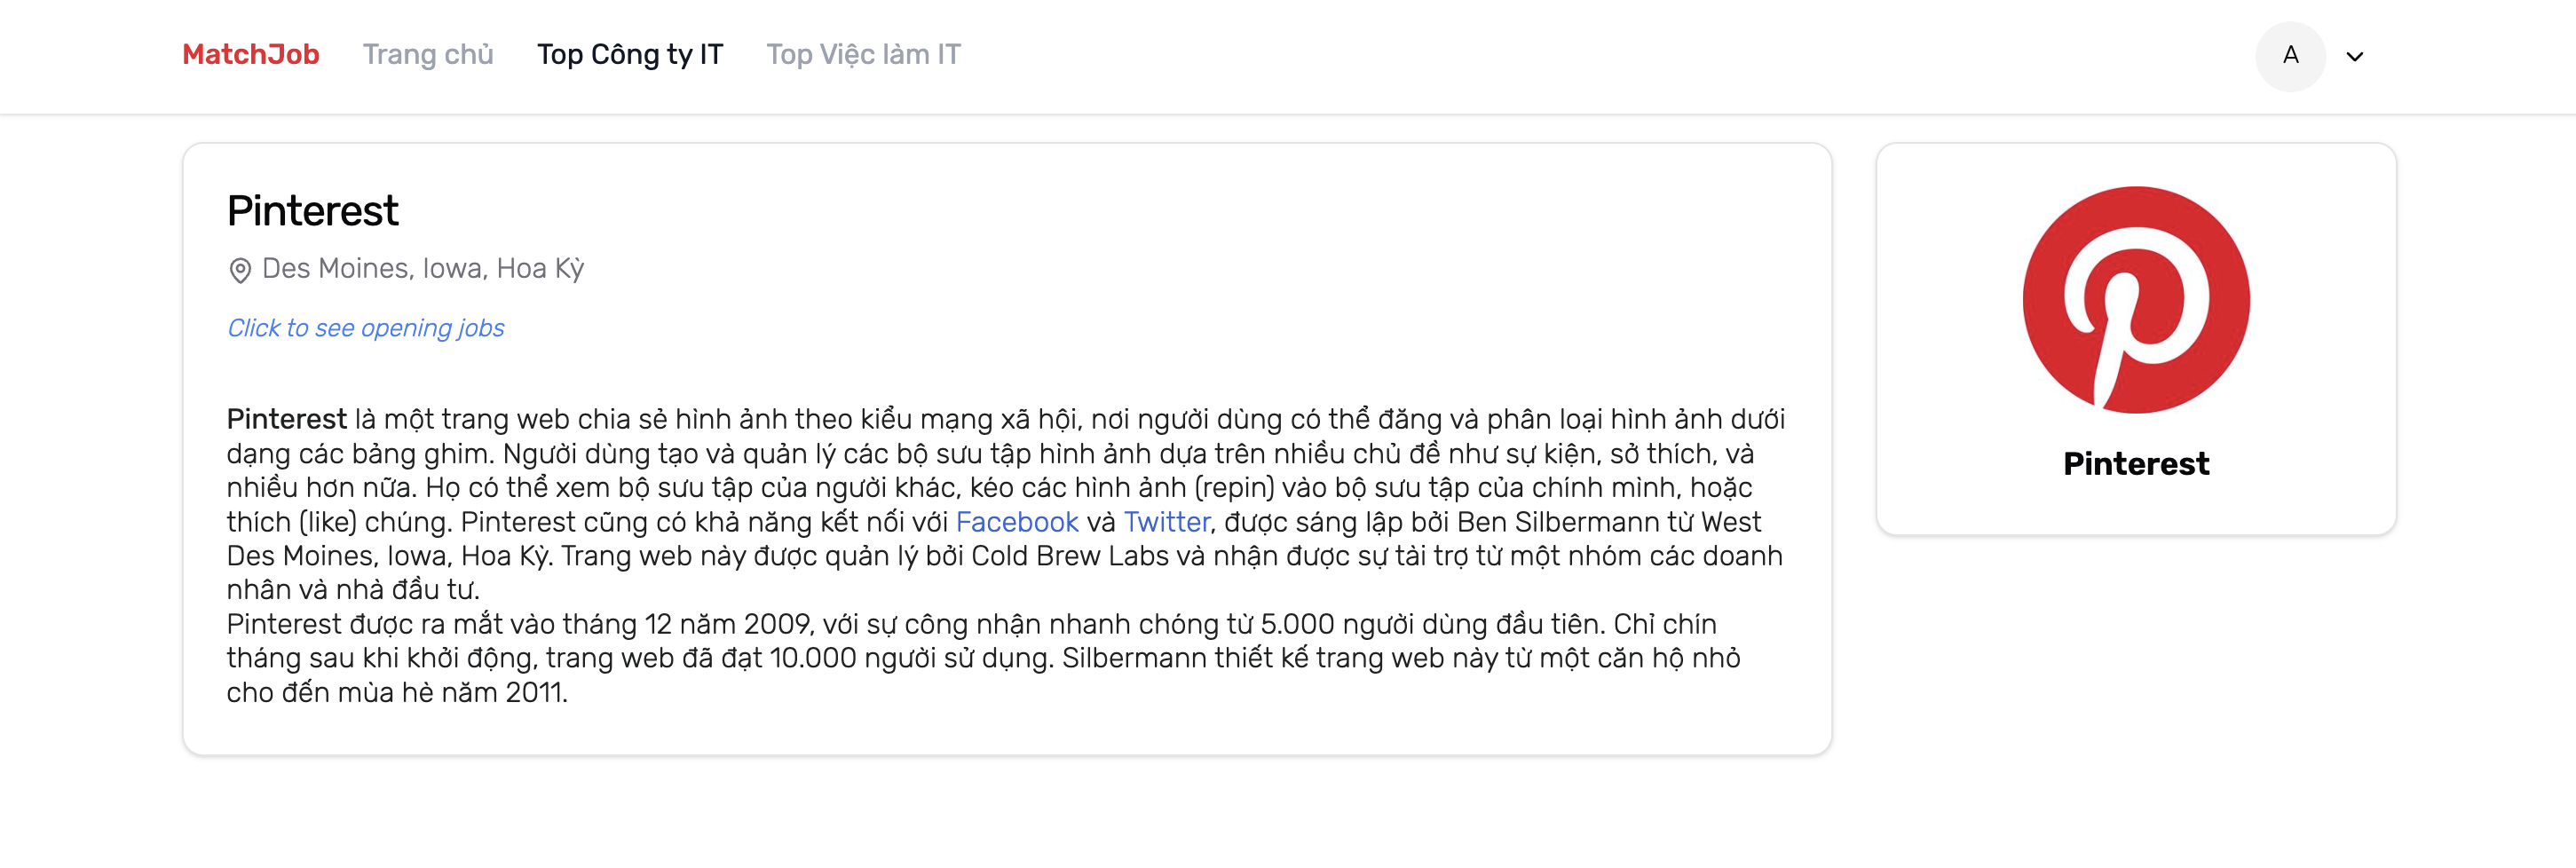
\includegraphics[width=\linewidth]{DBMS-Application/Images/company-detail.png}
    \caption{Thông tin chi tiết của công ty}
    \label{fig:enter-label}
\end{figure}

Truy vấn sử dụng: \textbf{Query with single condition} - Sử dụng điều kiện \texttt{\_id} để tìm công ty duy nhất

\begin{lstlisting}
return await this.db
  .collection('companies')
  .findOne({ _id: new ObjectId(id) }); // Chuyen id truyen vao thanh ObjectId, phu hop voi MongoDB
\end{lstlisting}

Ngoài ra, người dùng cũng có thể xem các công việc hiện đang được tuyển dụng của công ty này thông qua API lọc ra công việc của một công ty cụ thể (đã trình bày ở phần Trang chủ), hệ thống sẽ hiện lên 1 popup chứa các công việc của công ty hiện tại như sau:

\begin{figure}[H]
    \centering
    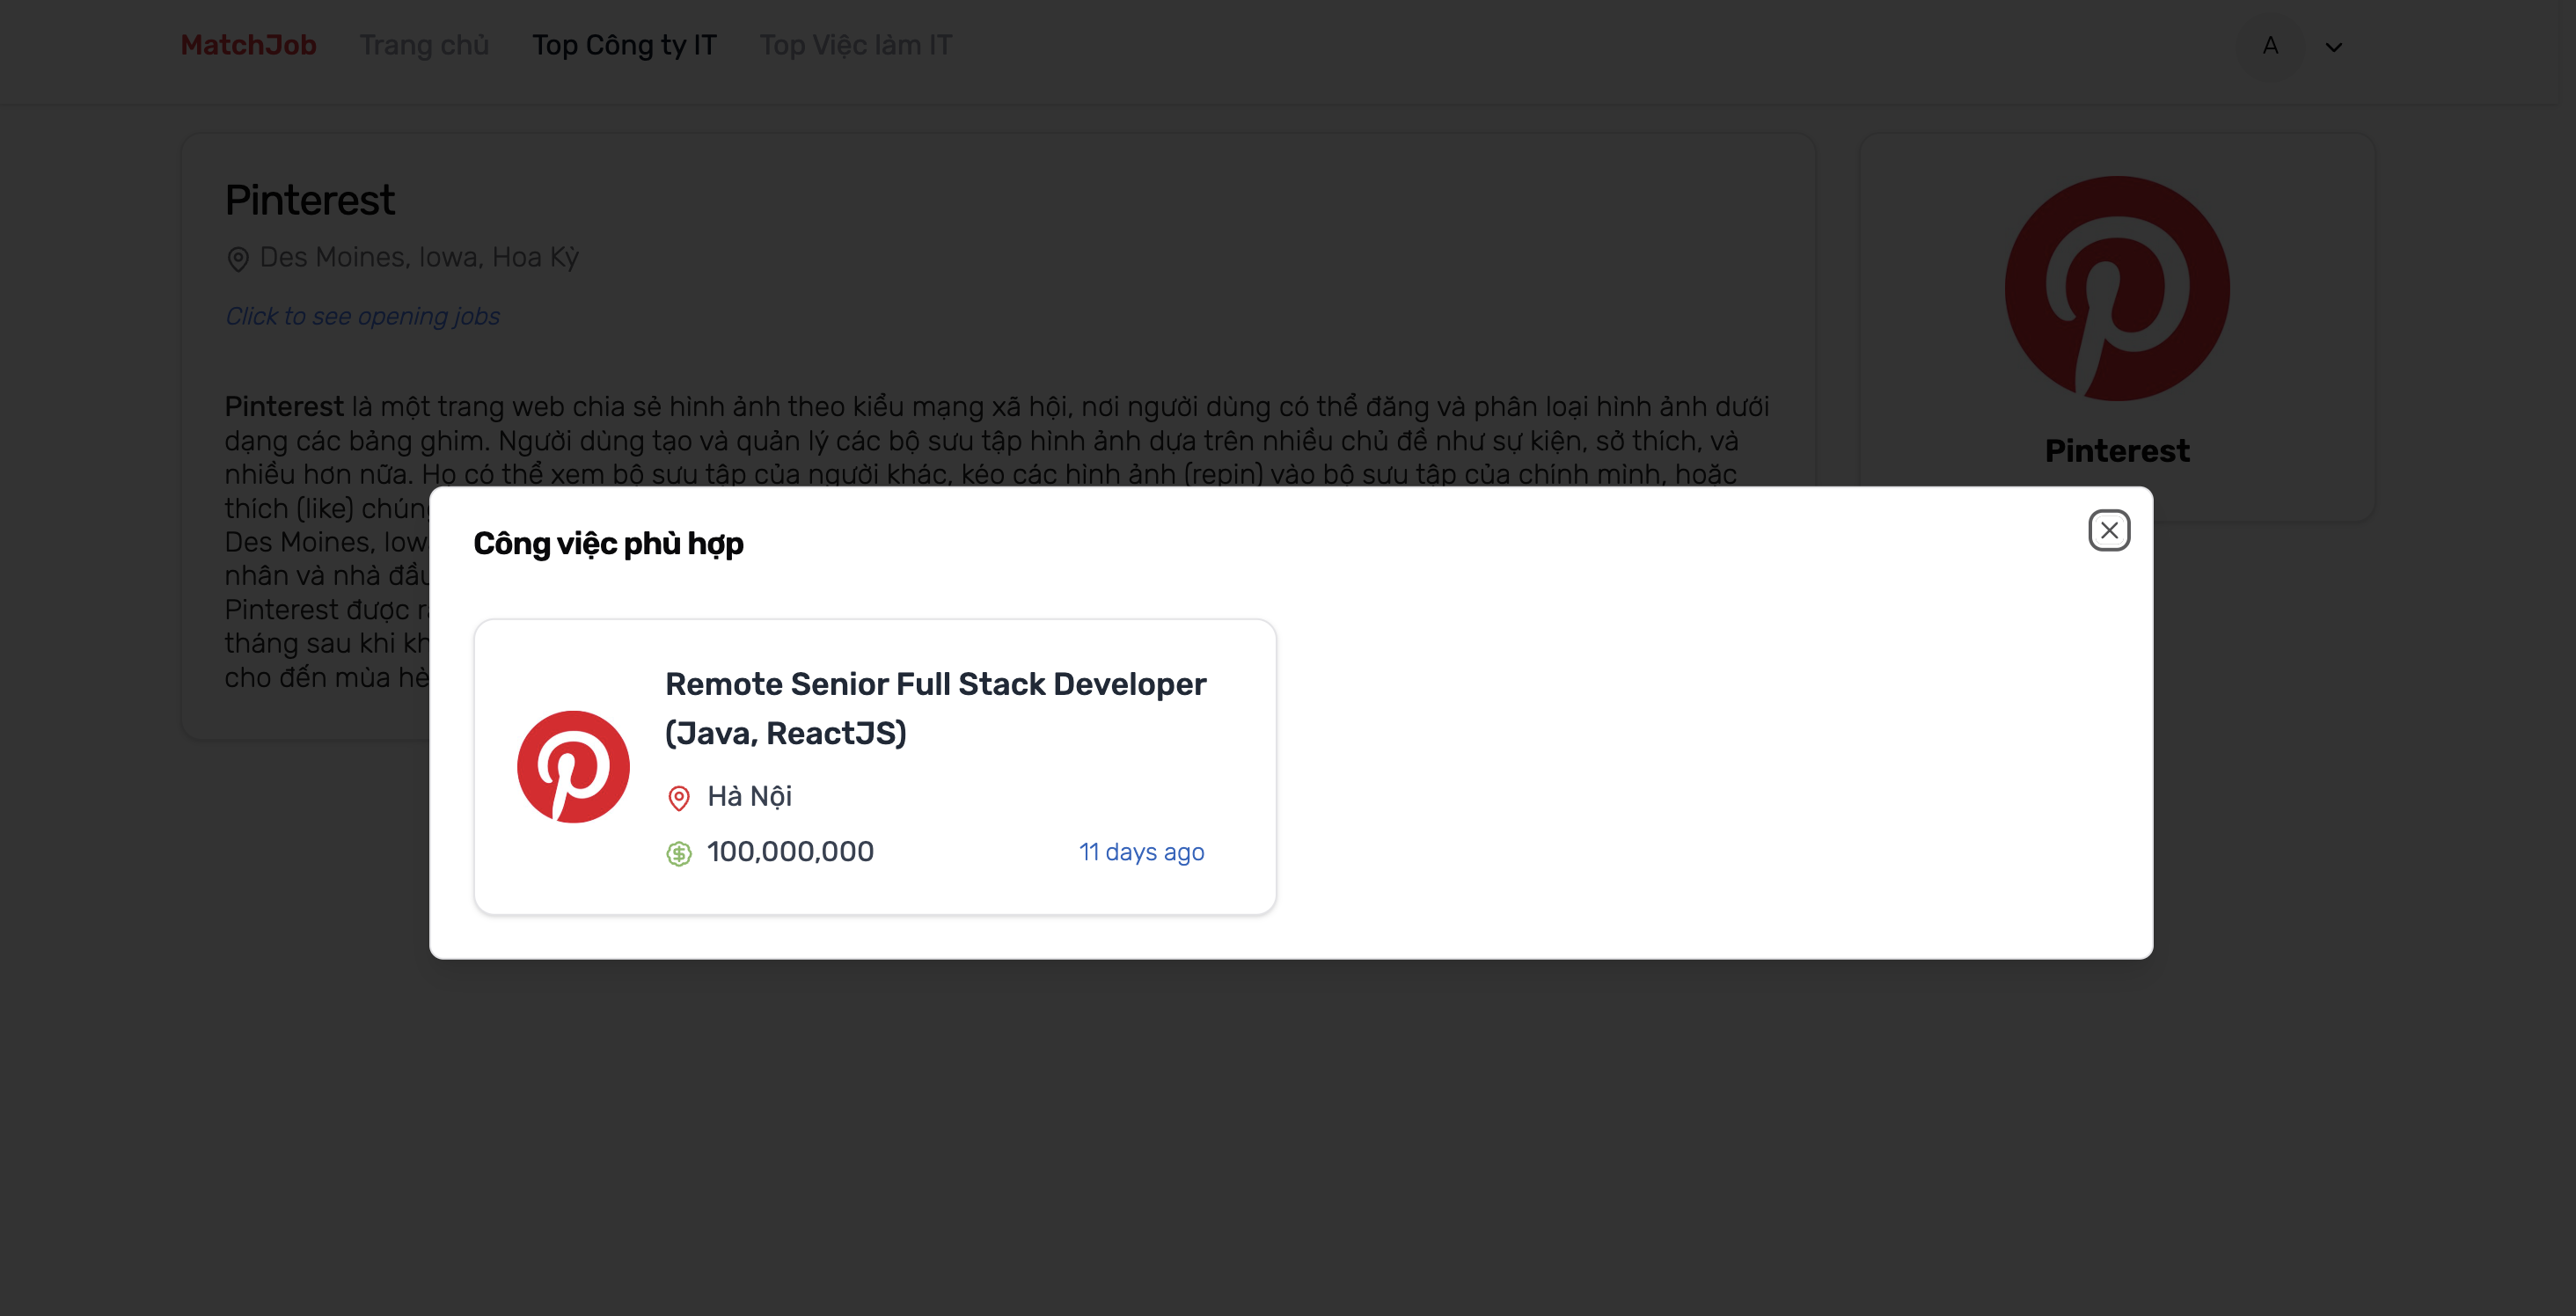
\includegraphics[width=\linewidth]{DBMS-Application/Images/modal-job-in-company-detail.png}
    \caption{Các công việc đang tuyển dụng của công ty cụ thể}
    \label{fig:enter-label}
\end{figure}




% \subsubsection{Giao diện người dùng - Danh sách/Chi tiết công việc}

Khi truy cập vào trang danh sách công việc tuyển dụng, Front-end sẽ tự động fetch dữ liệu từ Backend thông qua một API tương tự như ở trang chủ: thực hiện phân trang để lấy lần lượt các công việc trong cơ sở dữ liệu dựa trên tham số \texttt{current} và \texttt{pageSize}.

\begin{figure}[H]
    \centering
    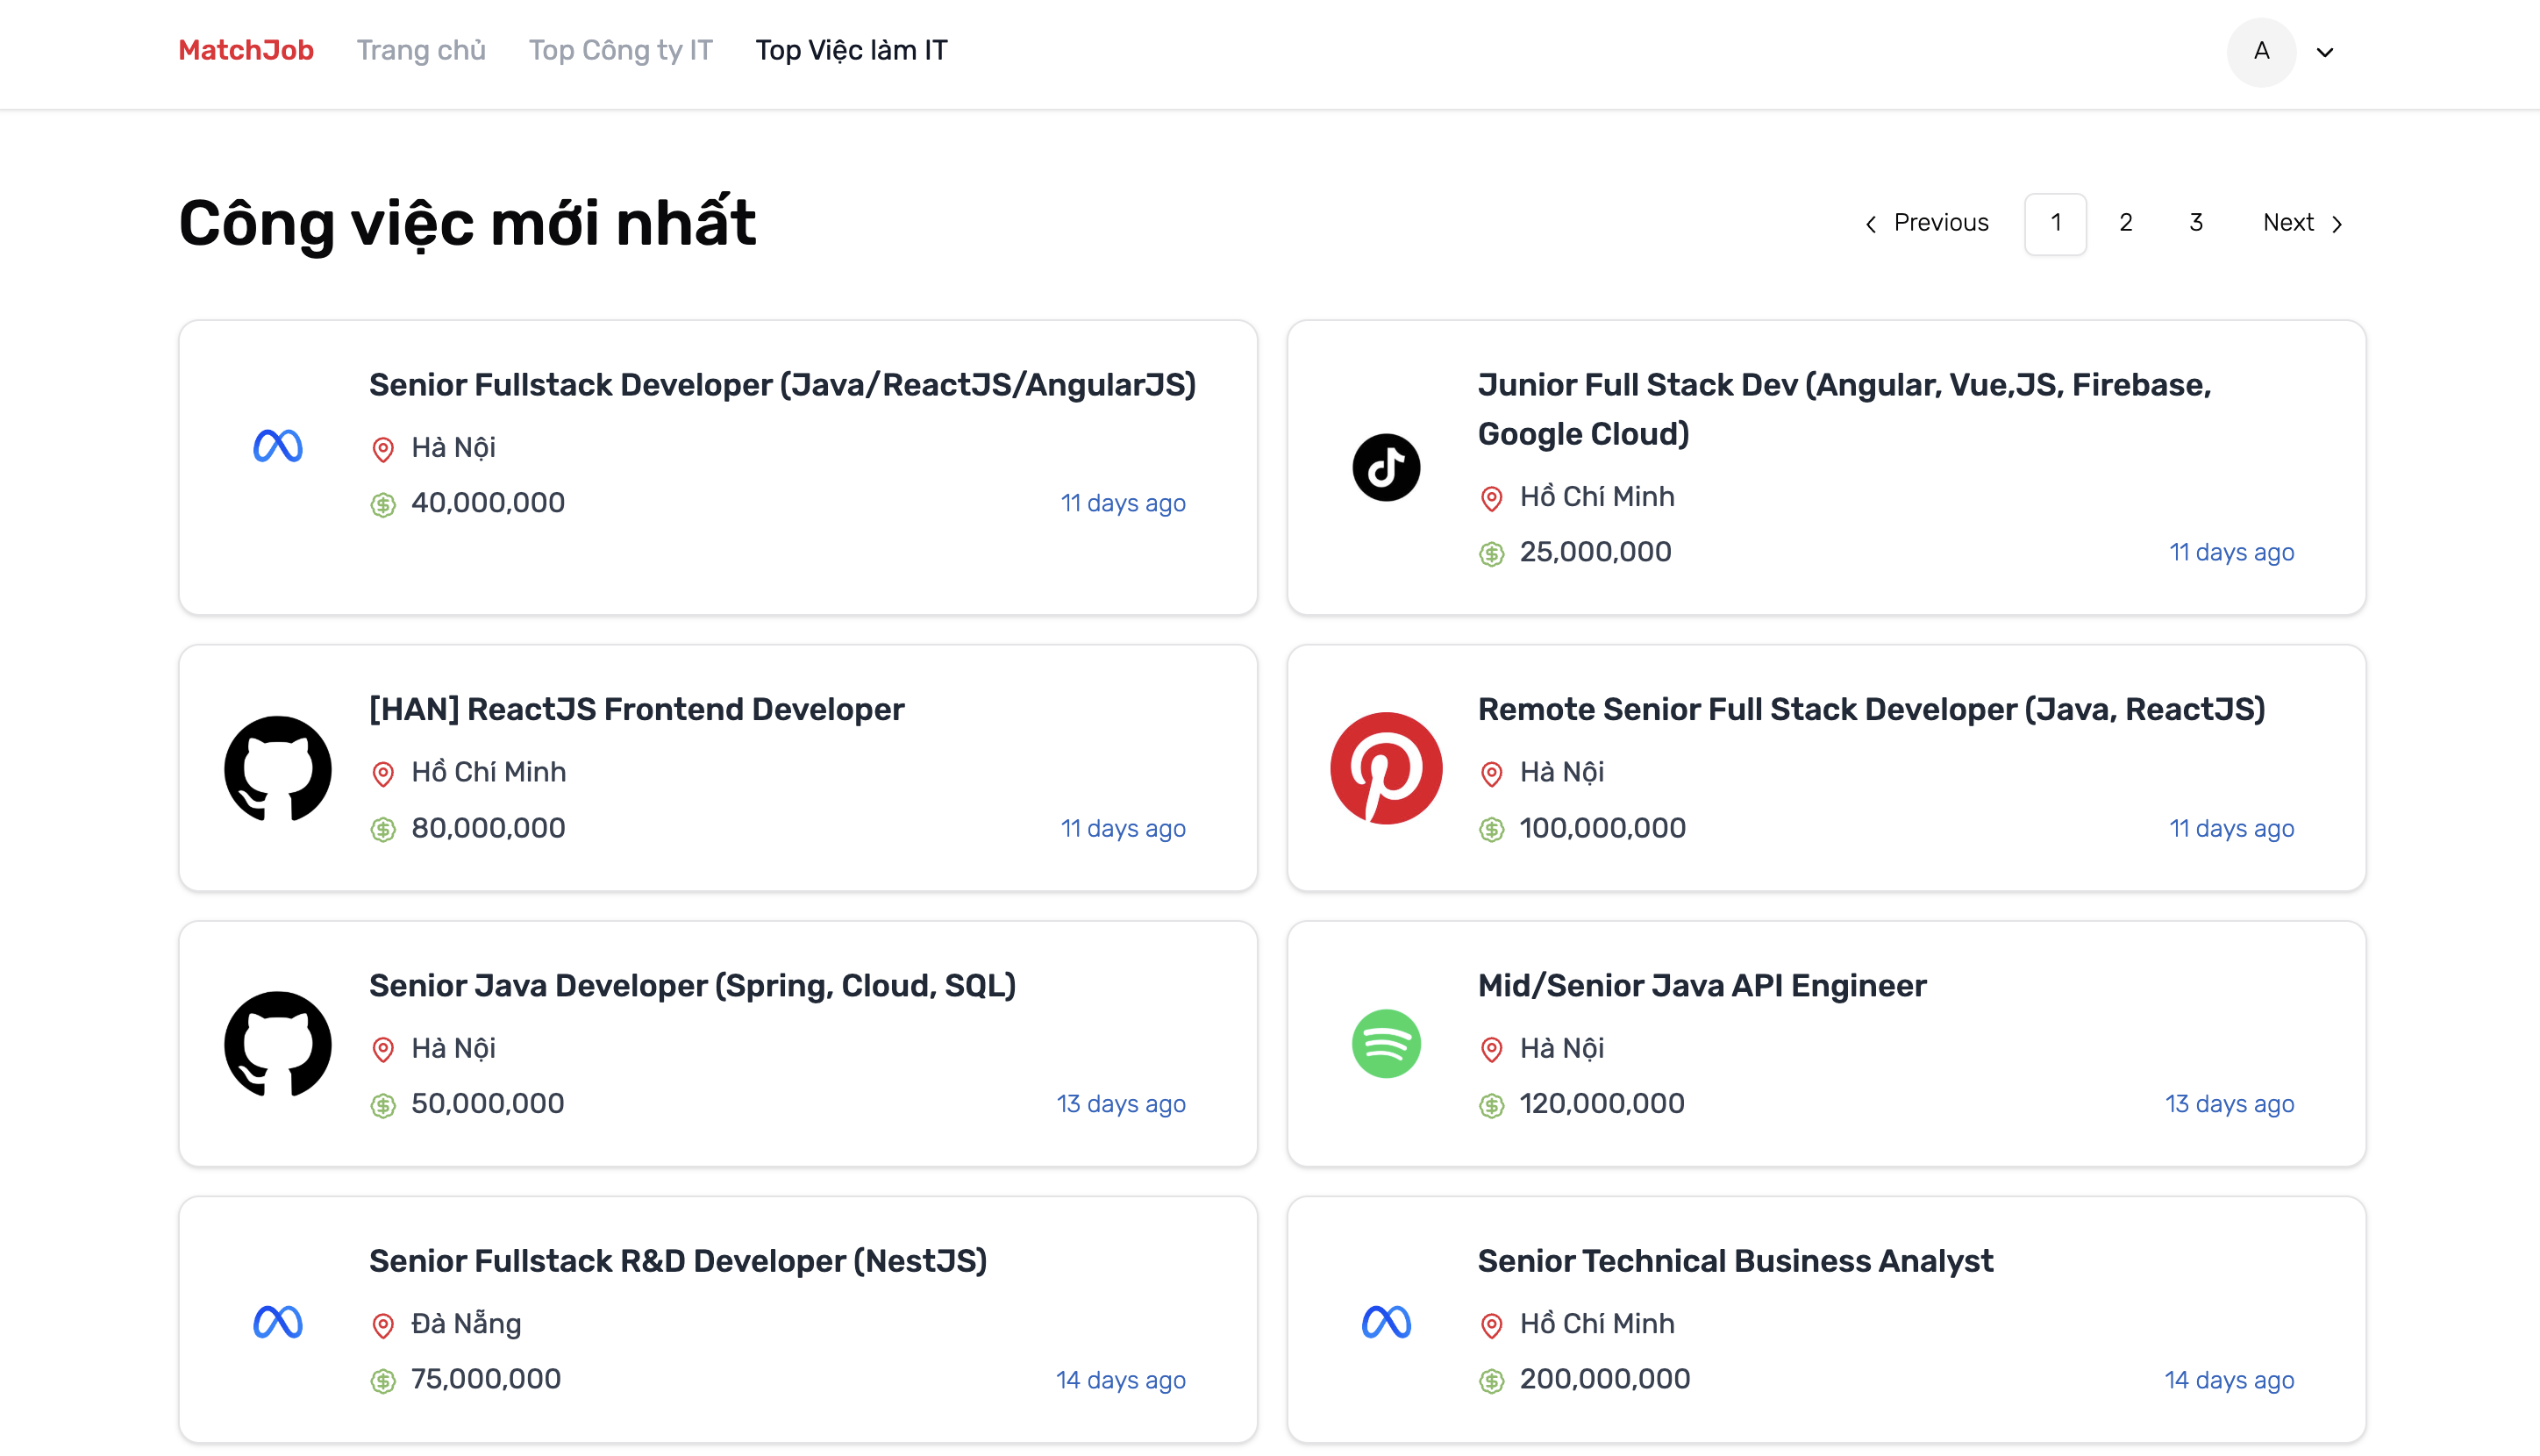
\includegraphics[width=\linewidth]{DBMS-Application/Images/list-job.png}
    \caption{Danh sách công việc đang được tuyển dụng}
\end{figure}

Và cũng như ở trang Danh sách công ty đã trình bày, người dùng cũng có thể chọn 1 công việc để xem chi tiết công việc đó:

\begin{figure}[H]
    \centering
    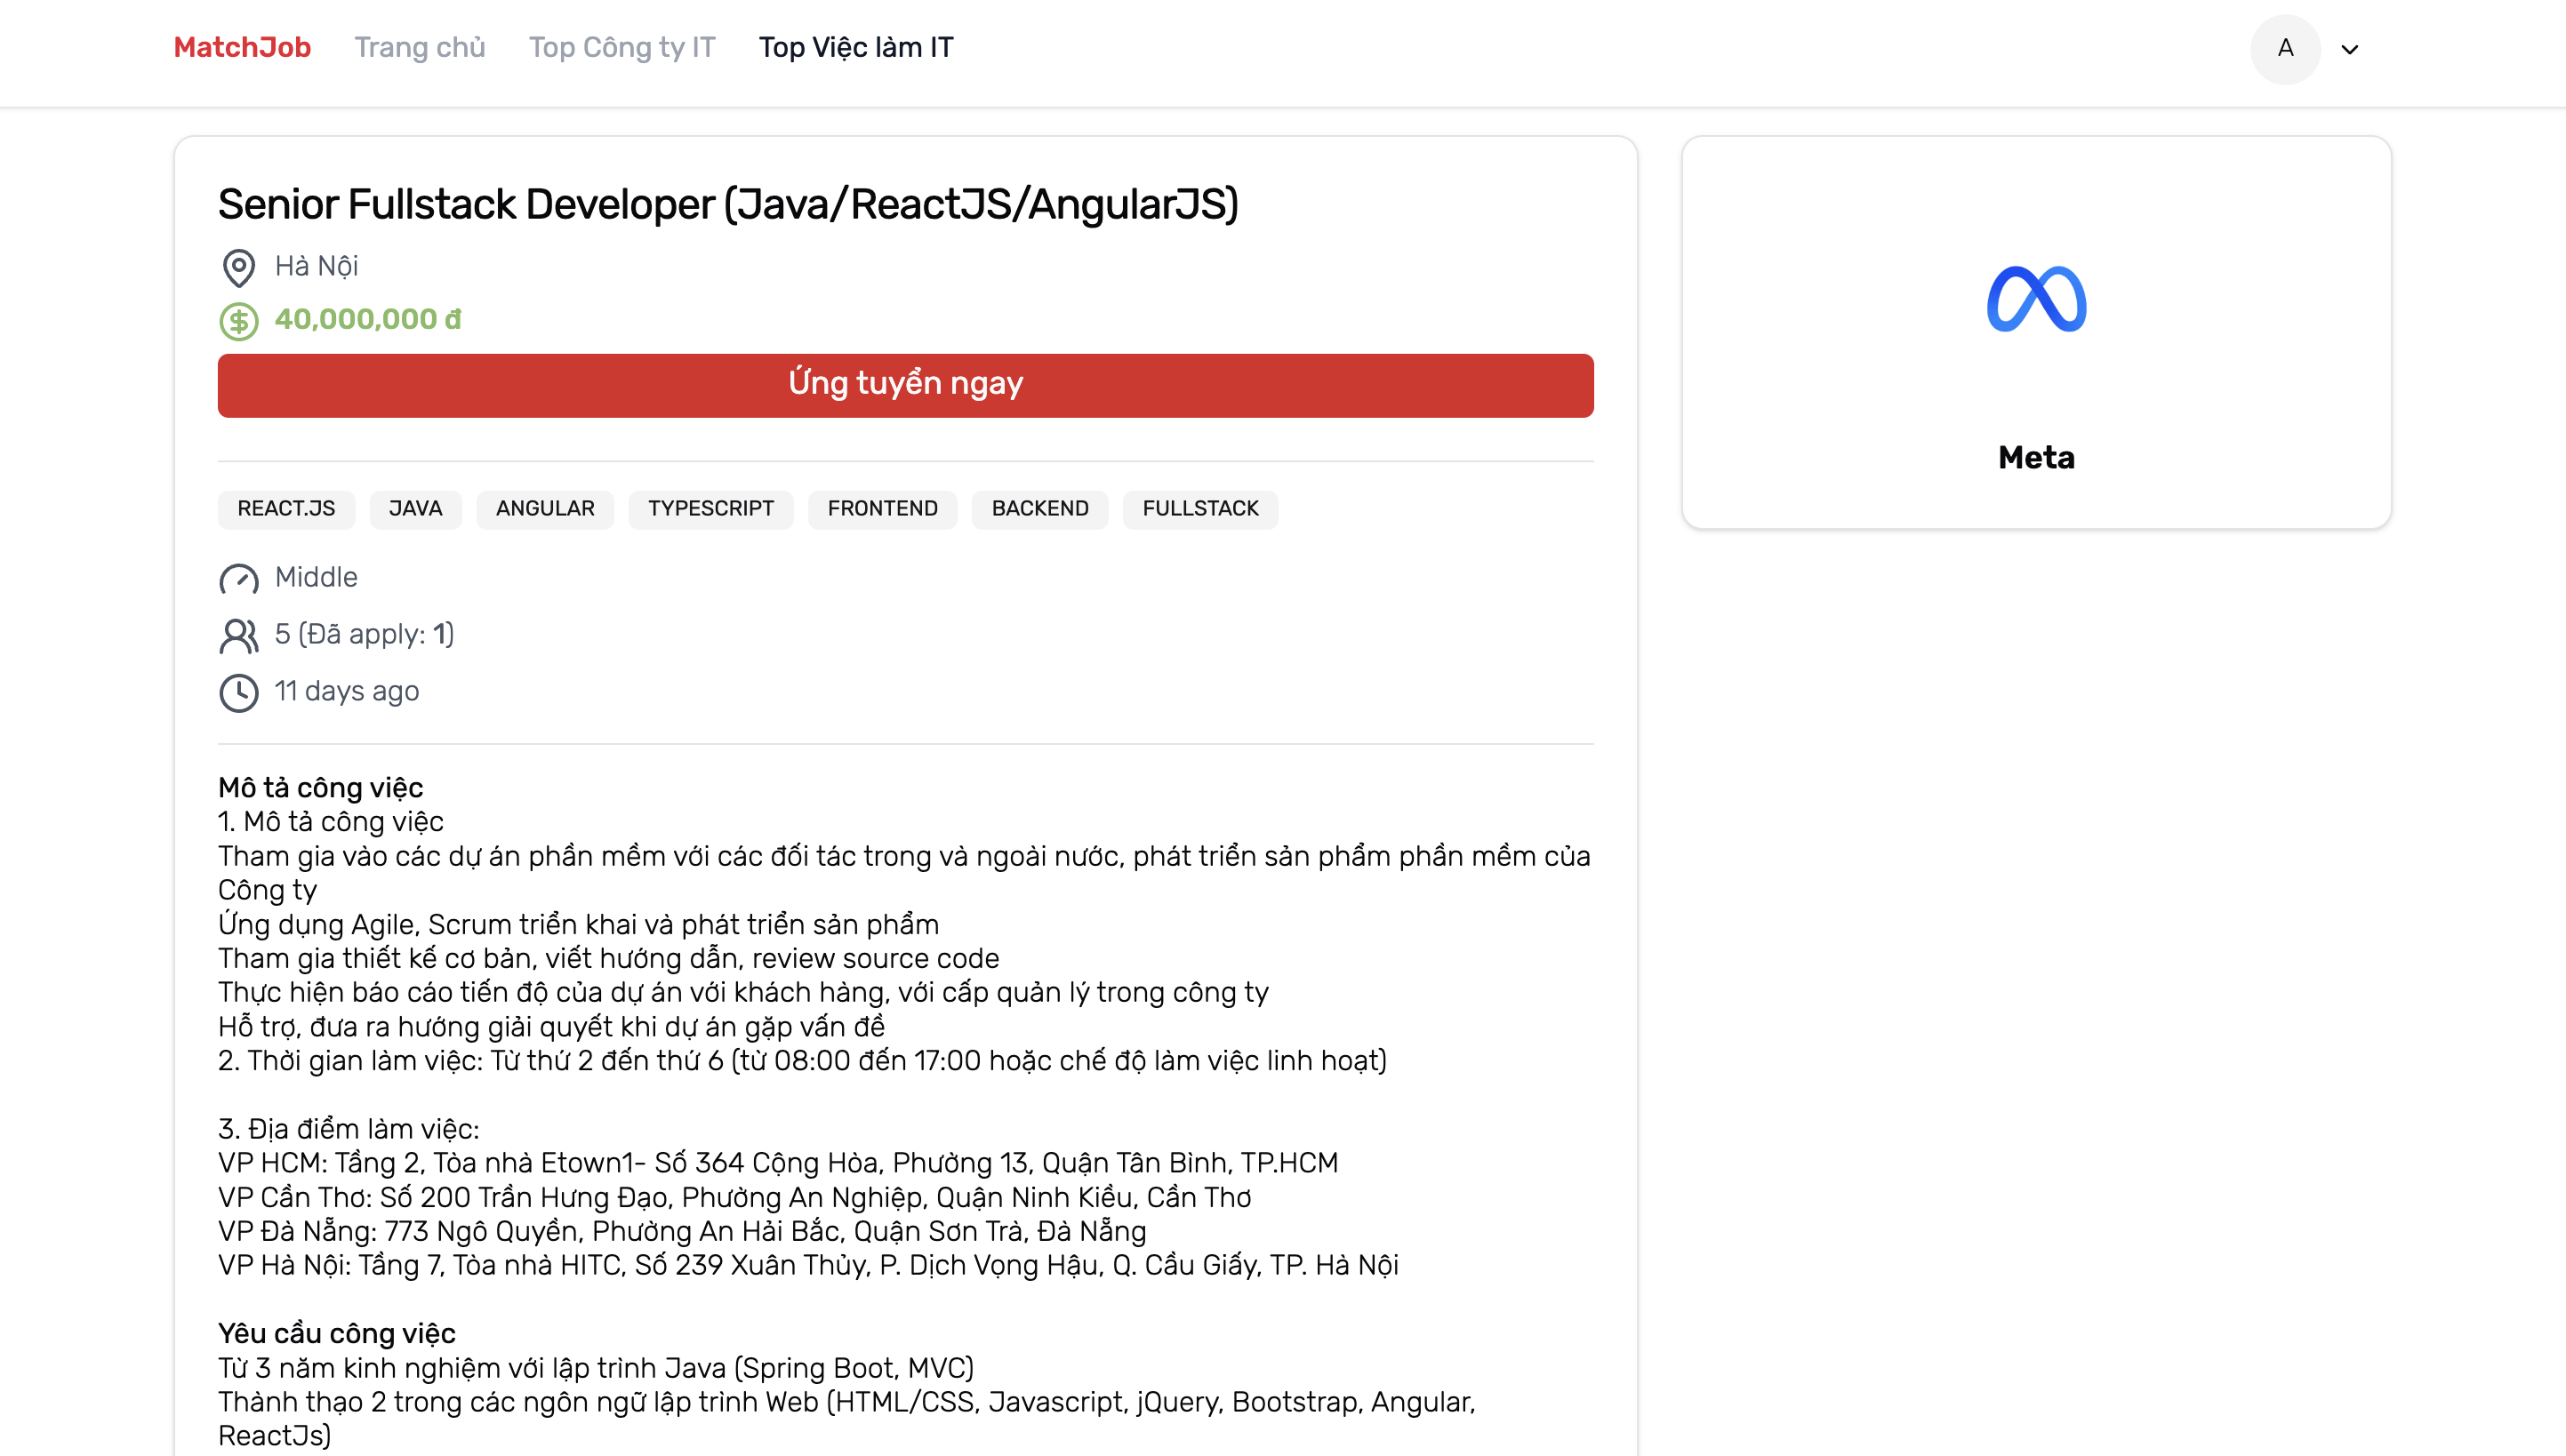
\includegraphics[width=\linewidth]{DBMS-Application/Images/job-detail.png}
    \caption{Danh sách công việc đang được tuyển dụng}
\end{figure}

Truy vấn sử dụng: \textbf{Query with single condition} - Sử dụng điều kiện \texttt{\_id} để tìm công việc duy nhất

\begin{lstlisting}
return await this.db
  .collection('jobs')
  .findOne({ _id: new ObjectId(id) });
\end{lstlisting}

Bên cạnh đó, hệ thống Front-end cũng tự động gửi yêu cầu thông qua API để lấy về số lượng hồ sơ đã nộp từ các ứng viên khác cho công việc hiện tại

\begin{figure}[H]
    \centering
    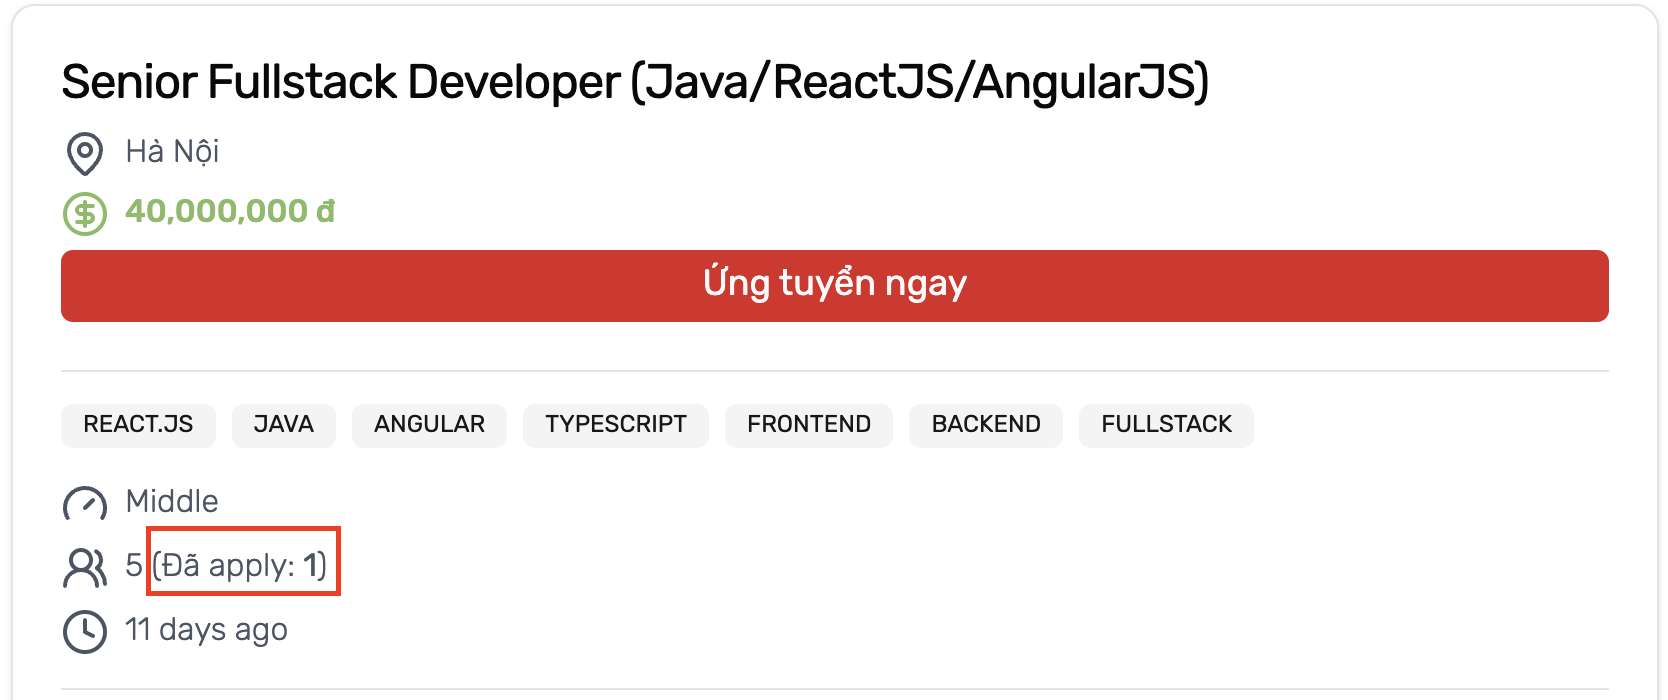
\includegraphics[width=.75\linewidth]{DBMS-Application/Images/number-resumes-apply.png}
    \caption{Số lượng hồ sơ đã được nộp cho công việc hiện tại}
\end{figure}

Truy vấn sử dụng:
\begin{itemize}
    \item \textbf{Query with single condition}: Sử dụng \texttt{\$match} để tìm một công việc cụ thể trong collection \textbf{jobs} dựa trên \texttt{\_id}
    
    \item \textbf{Query with join}: Thực hiện join thông qua \texttt{\$lookup} giữa collection \textbf{jobs} (\texttt{\_id}) và \textbf{resumes} (\texttt{jobId}) để lấy danh sách hồ sơ ứng tuyển của đến công việc đó

    \item \textbf{Query with aggregation functions}: Sử dụng \texttt{\$size} để tính tổng số lượng hồ sơ ứng tuyển của công việc
\end{itemize}

\begin{lstlisting}
const pipeline = [
  {
    $match: { _id: new ObjectId(id) }, // Tim job cu the thong qua _id
  },
  {
    $lookup: {
      from: 'resumes', // Join collection 'jobs' voi collection 'resumes'
      localField: '_id',
      foreignField: 'jobId',
      as: 'resumes',
    },
  },
  {
    $project: {
      _id: 1,
      totalResumes: { $size: '$resumes' }, // Dem so luong resumes da nop
    },
  },
];

const result = await this.db
  .collection('jobs')
  .aggregate(pipeline)
  .toArray();

return result[0];
\end{lstlisting}

Giải thích truy vấn:
\begin{itemize}
    \item \texttt{\$match}: Lọc công việc cụ thể từ collection \textbf{jobs} dựa trên \_id.
    \item \texttt{\$lookup}: Join với collection \textbf{resumes} để tìm các hồ sơ ứng tuyển có trường \texttt{jobId} trùng với \texttt{\_id} của công việc
    \item \texttt{\$project}: Trả về \texttt{\_id} của công việc và tổng số hồ sơ ứng tuyển (\texttt{totalResumes}) bằng cách sử dụng \texttt{\$size} để đếm số phần tử trong mảng resumes.
\end{itemize}

Cuối cùng, người dùng có thể upload (tạo) hồ sơ và apply cho công việc cụ thể:

\begin{figure}[H]
    \centering
    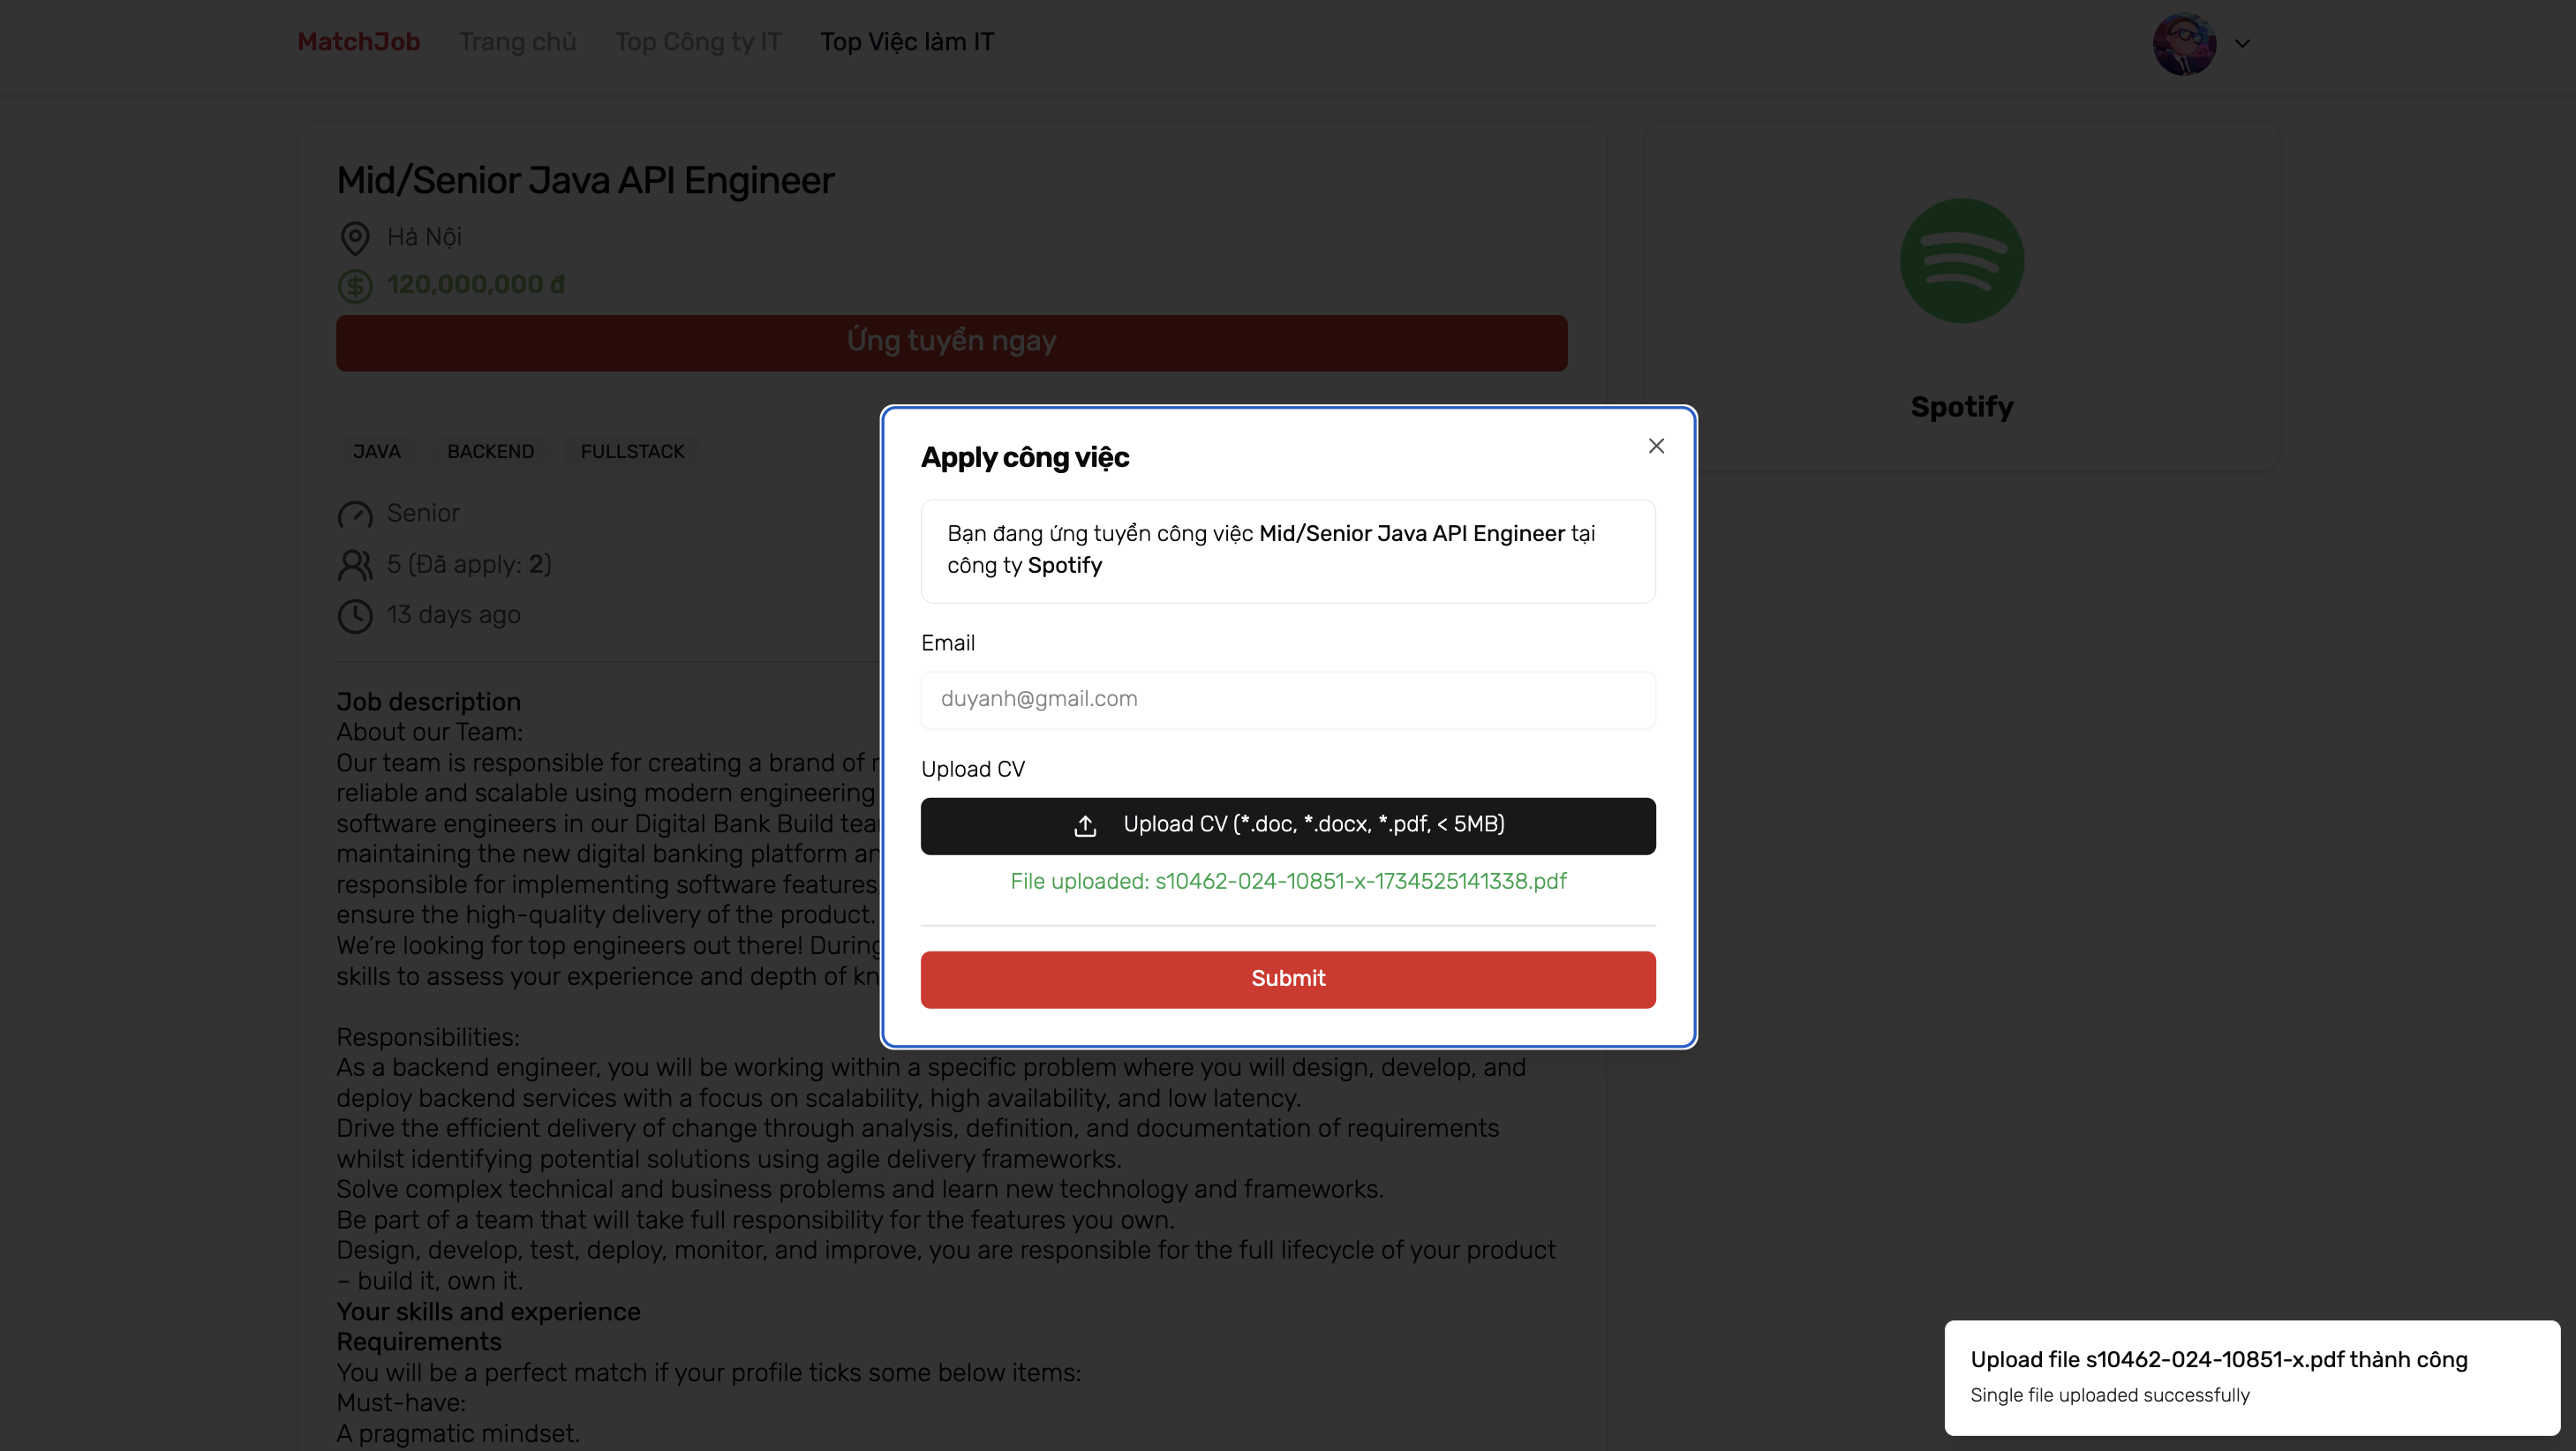
\includegraphics[width=\linewidth]{DBMS-Application/Images/modal-upload-cv.png}
    \caption{Số lượng hồ sơ đã được nộp cho công việc hiện tại}
\end{figure}

Truy vấn sử dụng: \textbf{Insert}

\begin{lstlisting}
const newResume = {
  url,
  companyId: new ObjectId(companyId),
  email,
  jobId: new ObjectId(jobId),
  userId: new ObjectId(_id),
  status: 'PENDING',
  createdAt: new Date(),
  updatedAt: new Date(),
};

const result = await this.db.collection('resumes').insertOne(newResume); // Them ho so ung tuyen moi vao database

return {
  _id: result.insertedId,
  createdAt: newResume.createdAt,
};

\end{lstlisting}


% \subsubsection{Giao diện người dùng - Danh sách hồ sơ đã ứng tuyển}

Người dùng có thể xem lại các hồ sơ ứng tuyển của họ cho từng công việc:

\begin{figure}[H]
    \centering
    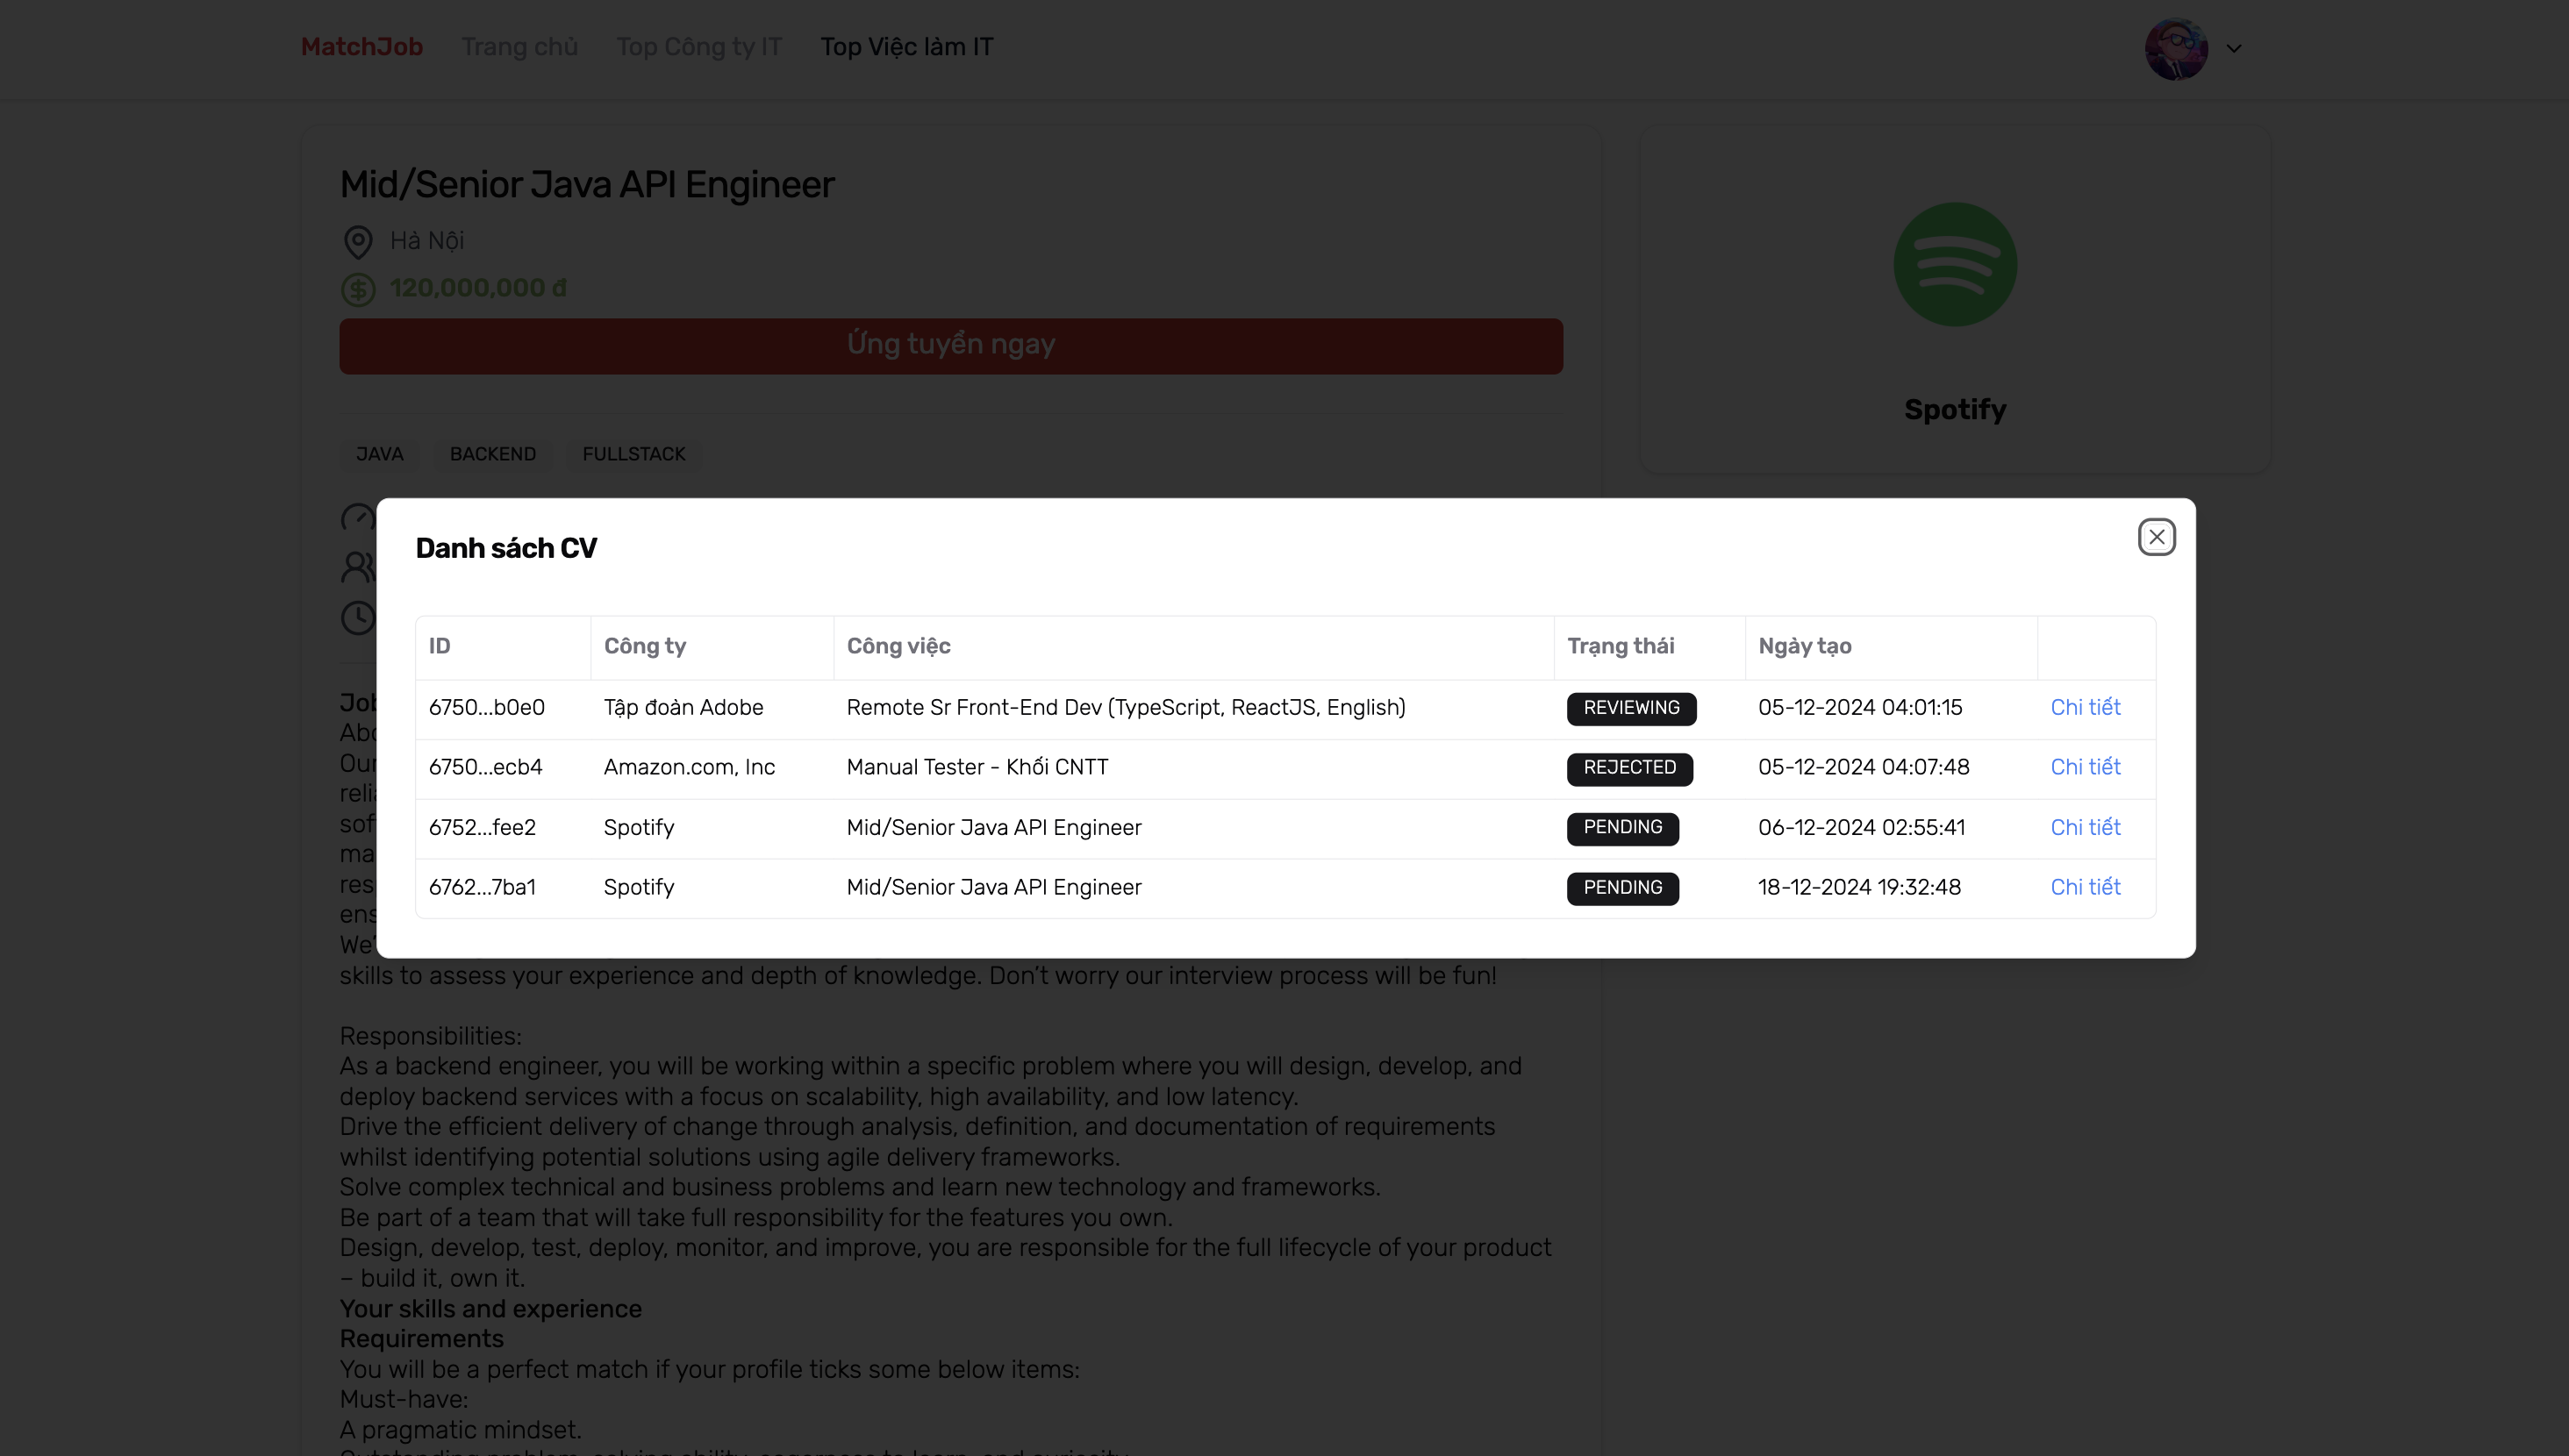
\includegraphics[width=\linewidth]{DBMS-Application/Images/modal-list-cv.png}
    \caption{Các hồ sơ đã được nộp của một người dùng}
\end{figure}

Truy vấn sử dụng:
\begin{itemize}
    \item \textbf{Query with join}: Sử dụng \texttt{\$lookup} để liên kết dữ liệu giữa hai collection \textbf{users} và \textbf{resumes}

    \item \textbf{Query with single condition}: Sử dụng \texttt{\$match} để lọc hồ sơ của của người dùng có \texttt{\_id}
\end{itemize}

\begin{lstlisting}
const result = await this.db
  .collection('users')
  .aggregate([
    {
      $lookup: {
        from: 'resumes',
        localField: '_id',
        foreignField: 'userId',
        as: 'userResumes',
      },
    },
    {
      $match: {
        _id: new ObjectId(user._id),
      },
    },
    {
      $project: {
        userResumes: 1,
      },
    },
  ])
  .toArray();

const resumes = result.length > 0 ? result[0].userResumes : [];
return resumes;
\end{lstlisting}

Giải thích truy vấn:
\begin{itemize}
    \item \texttt{\$lookup}: Thực hiện join giữa collection \textbf{users} và collection \textbf{resumes} để lấy tất cả các hồ sơ ứng tuyển của người dùng (\texttt{userId}) tương ứng với \texttt{\_id} của user.
    \item \texttt{\$match}: Lọc để chỉ lấy hồ sơ ứng tuyển của người dùng có \texttt{\_id} trùng với ID của user được truyền vào (\texttt{user.\_id}).
    \item \texttt{\$project}: Chỉ giữ lại trường \texttt{userResumes} trong kết quả trả về, ẩn các trường khác.
\end{itemize}

Truy vấn trả về mảng các hồ sơ ứng tuyển (\texttt{userResumes}) của người dùng (trả về mảng rỗng trong trường hợp người dùng chưa tải lên hồ sơ ứng tuyển nào)

% \subsubsection{Giao diện Admin - Quản lý công việc}

Trang quản lý công việc được thiết kế để hiển thị danh sách toàn bộ các công việc hiện có trong hệ thống, phục vụ việc quản lý, chỉnh sửa hoặc xóa công việc. Dữ liệu cũng được lấy từ Backend thông qua API theo cơ chế phân trang tương tự như các phần trước, giúp tối ưu hóa hiệu suất và hiển thị mượt mà, đặc biệt khi số lượng công việc lớn.

\begin{figure}[H]
    \centering
    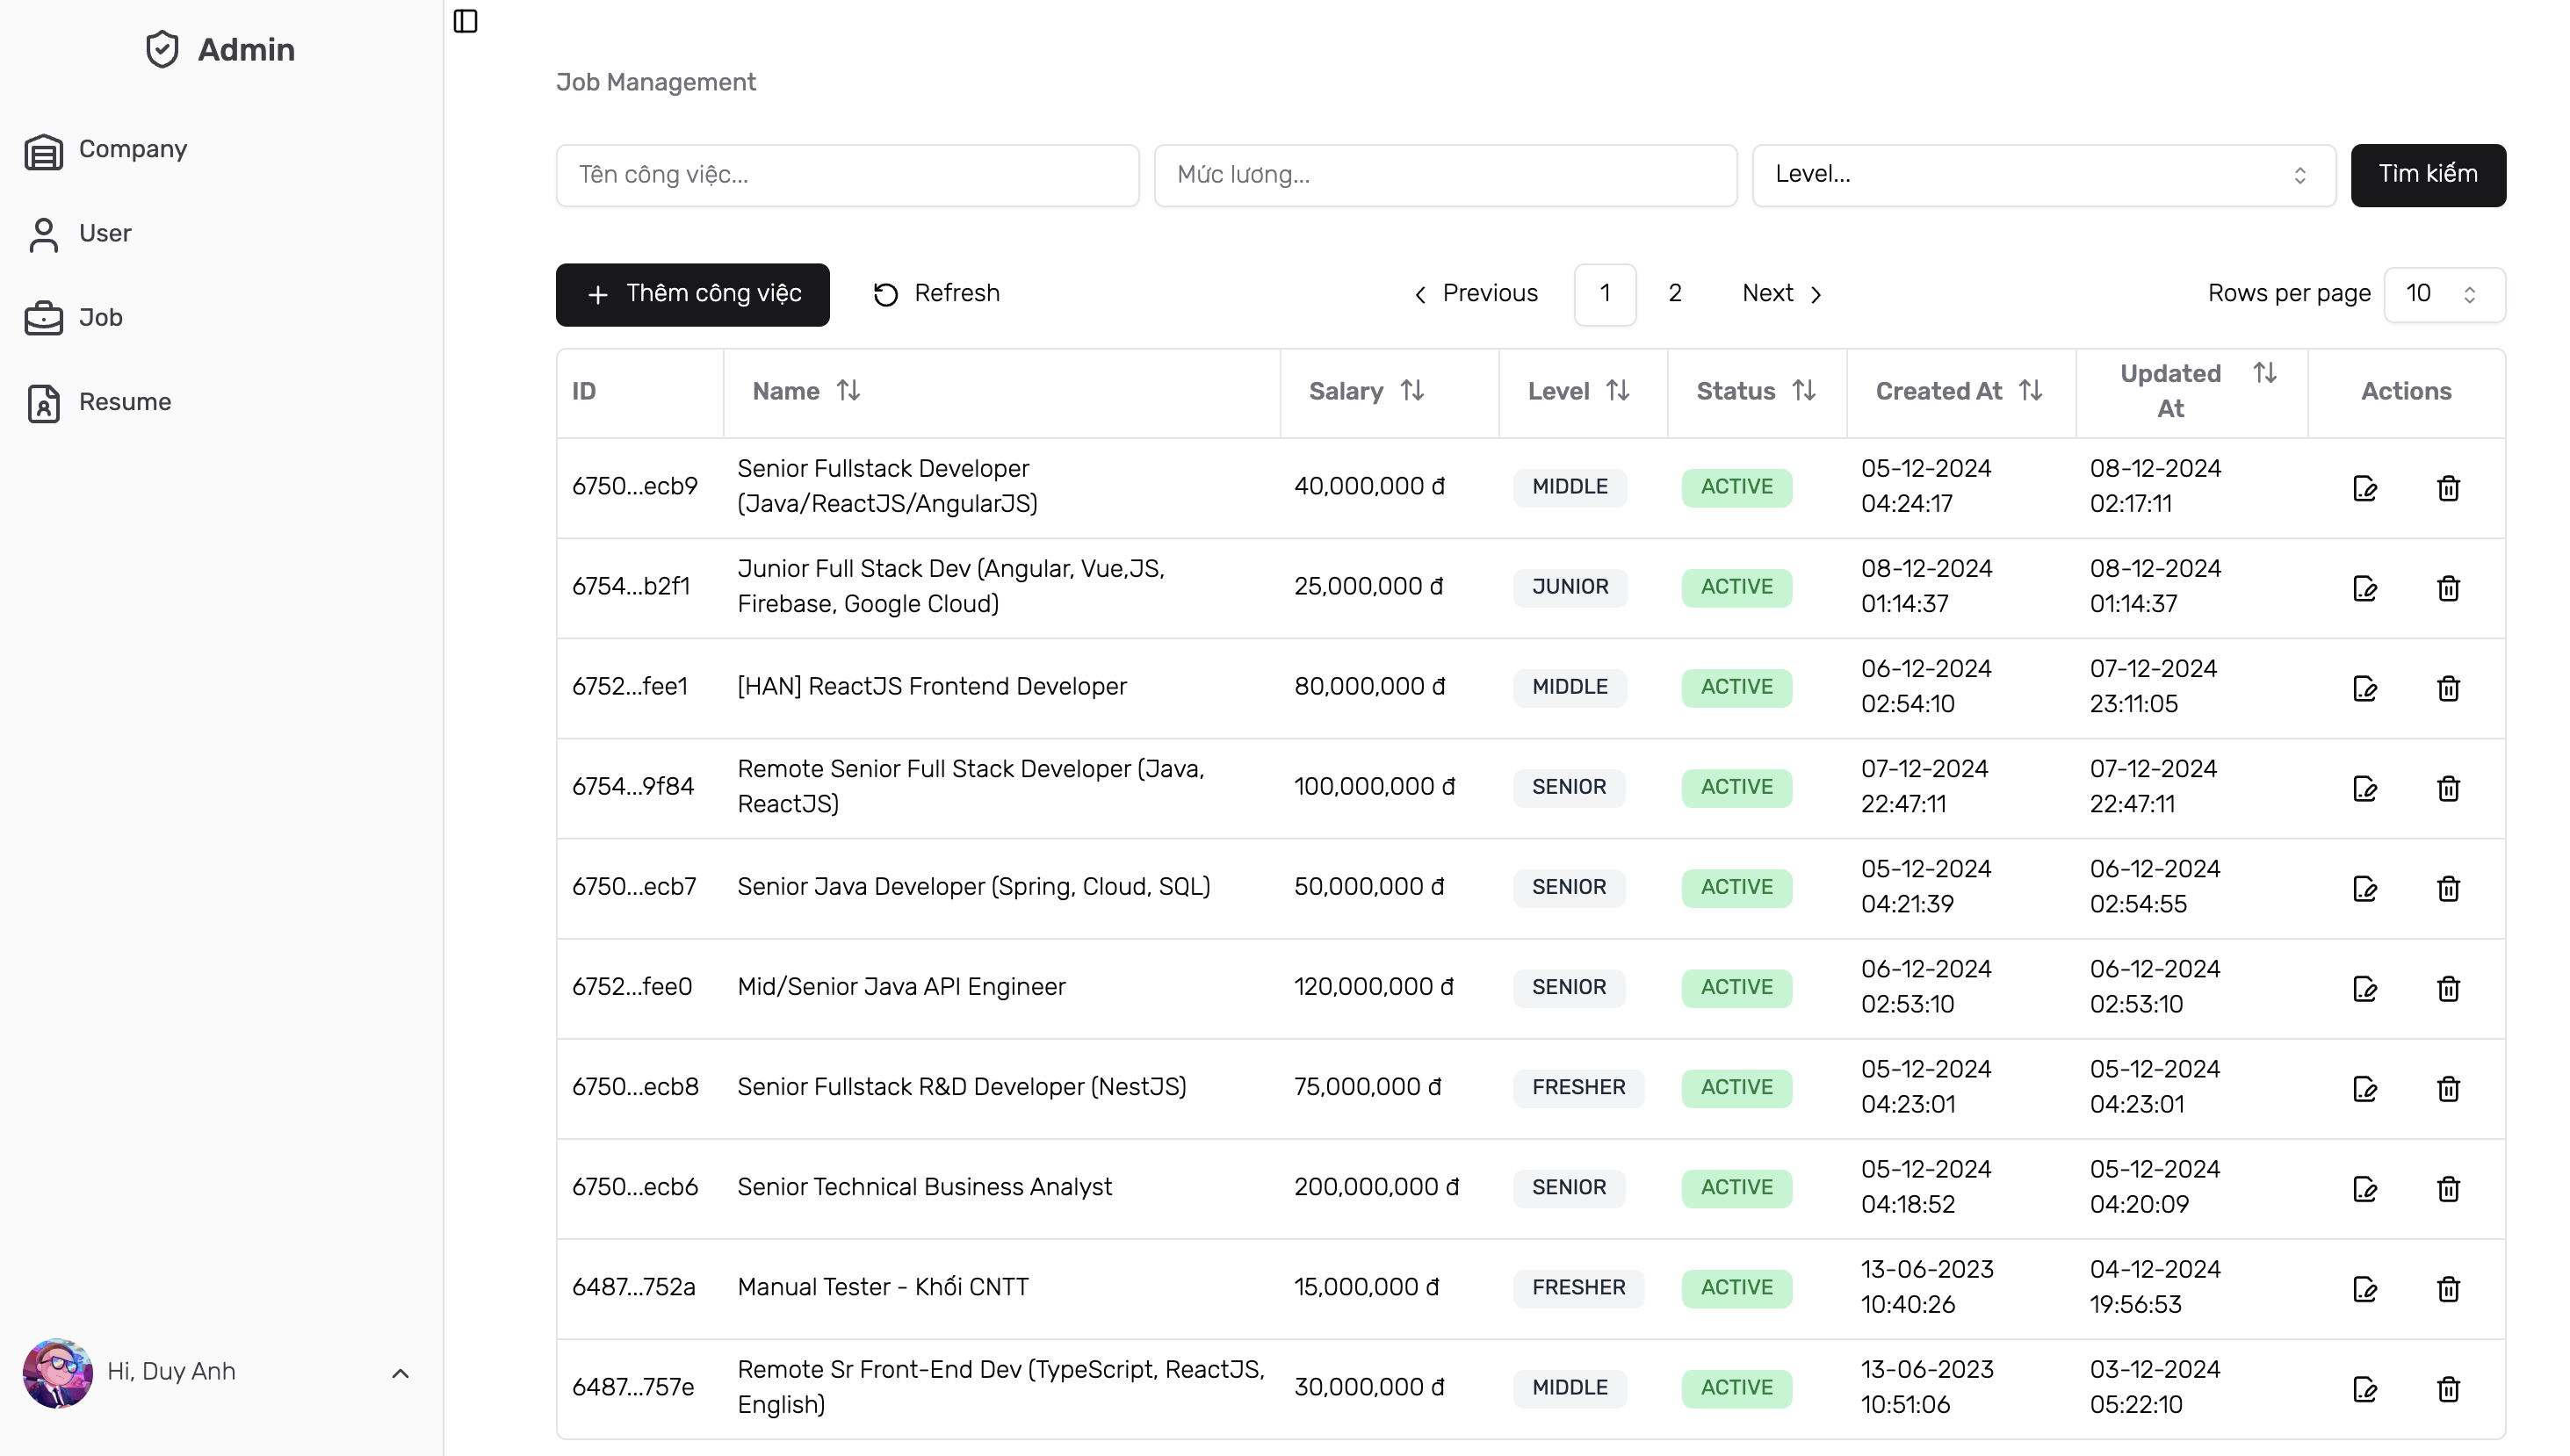
\includegraphics[width=\linewidth]{DBMS-Application/Images/admin-job.png}
    \caption{Trang quản lý công việc - Danh sách các công việc trong hệ thống}
    \label{fig:enter-label}
\end{figure}

Quản trị viên cũng có thể tìm kiếm và lọc ra các công ty theo \textbf{Tên}, \textbf{Mức lương} và \textbf{Level} như sau:

\begin{figure}[H]
    \centering
    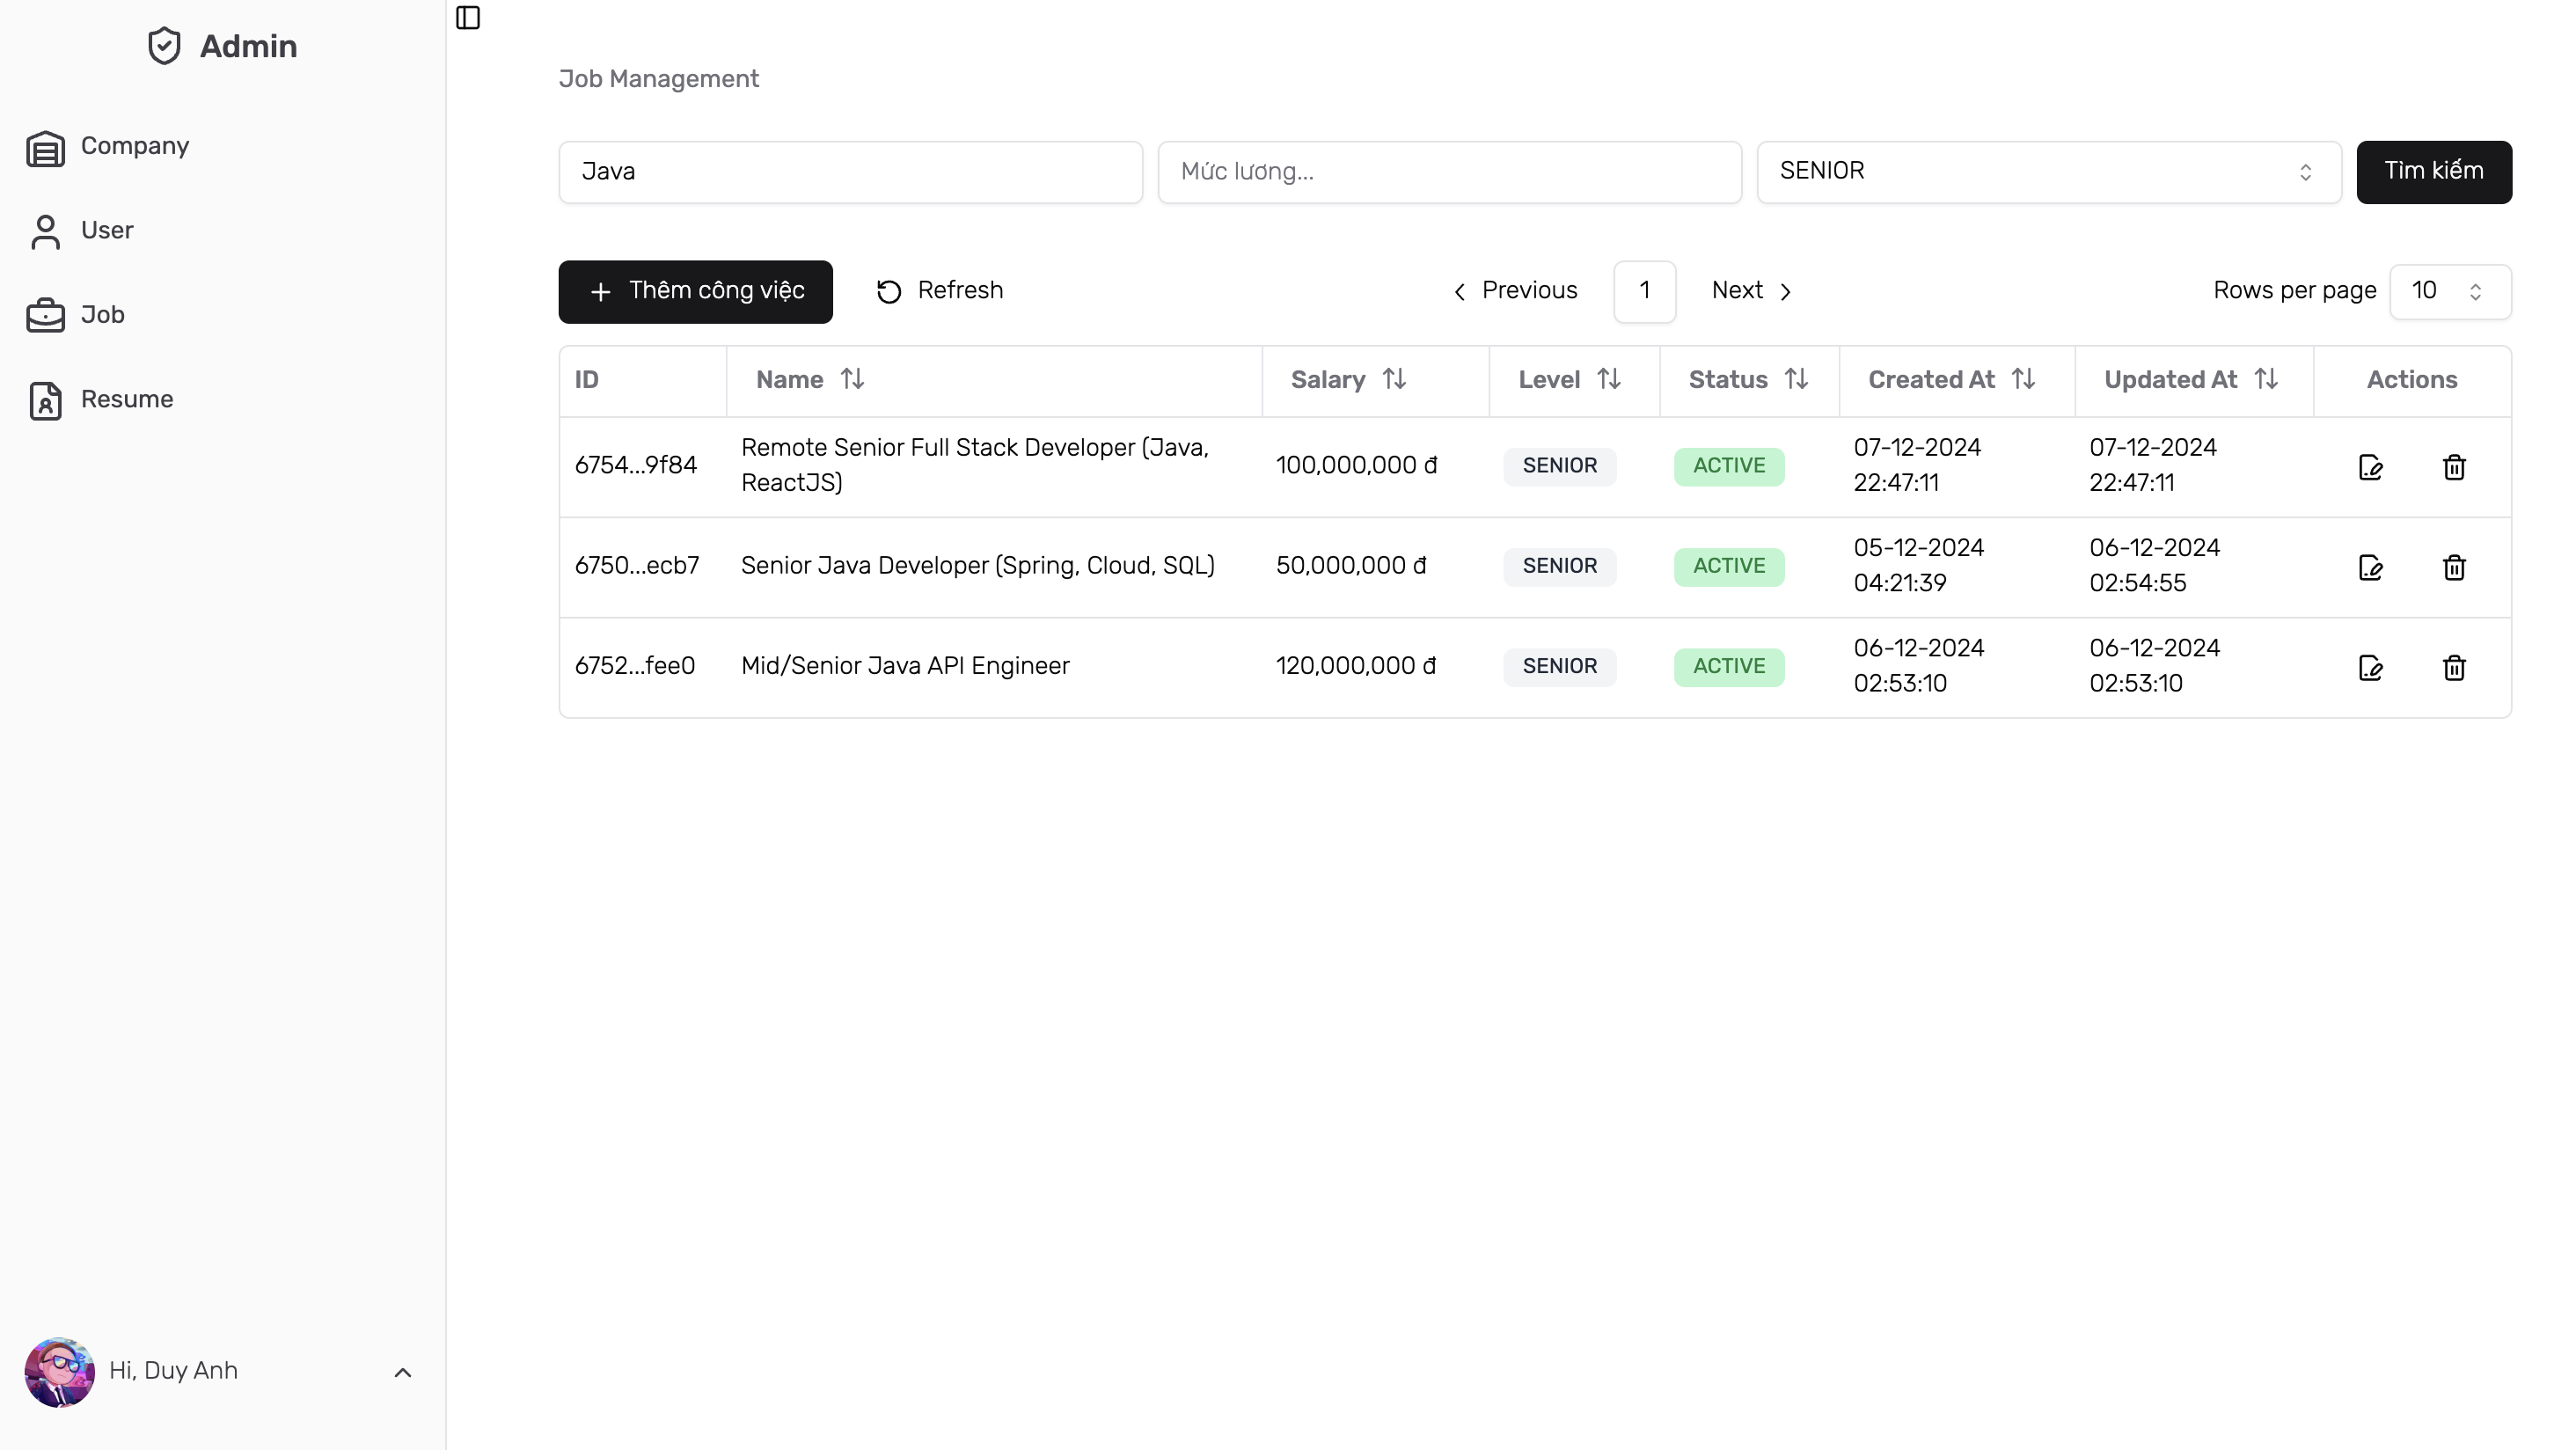
\includegraphics[width=\linewidth]{DBMS-Application/Images/admin-job-filter.png}
    \caption{Trang quản lý công việc - Danh sách công việc lọc theo điều kiện}
    \label{fig:enter-label}
\end{figure}

Truy vấn sử dụng: \textbf{Query with single/composite condition}\\

Bên cạnh đó, quản trị viên cũng có thể thêm công việc mới, bằng cách điền các thông tin cần thiết vào giao diện dưới đây. Sau đó, hệ thống sẽ gửi thông tin này đến cơ sở dữ liệu để thực hiện việc thêm document mới vào collection \textbf{jobs}.

\begin{figure}[H]
    \centering
    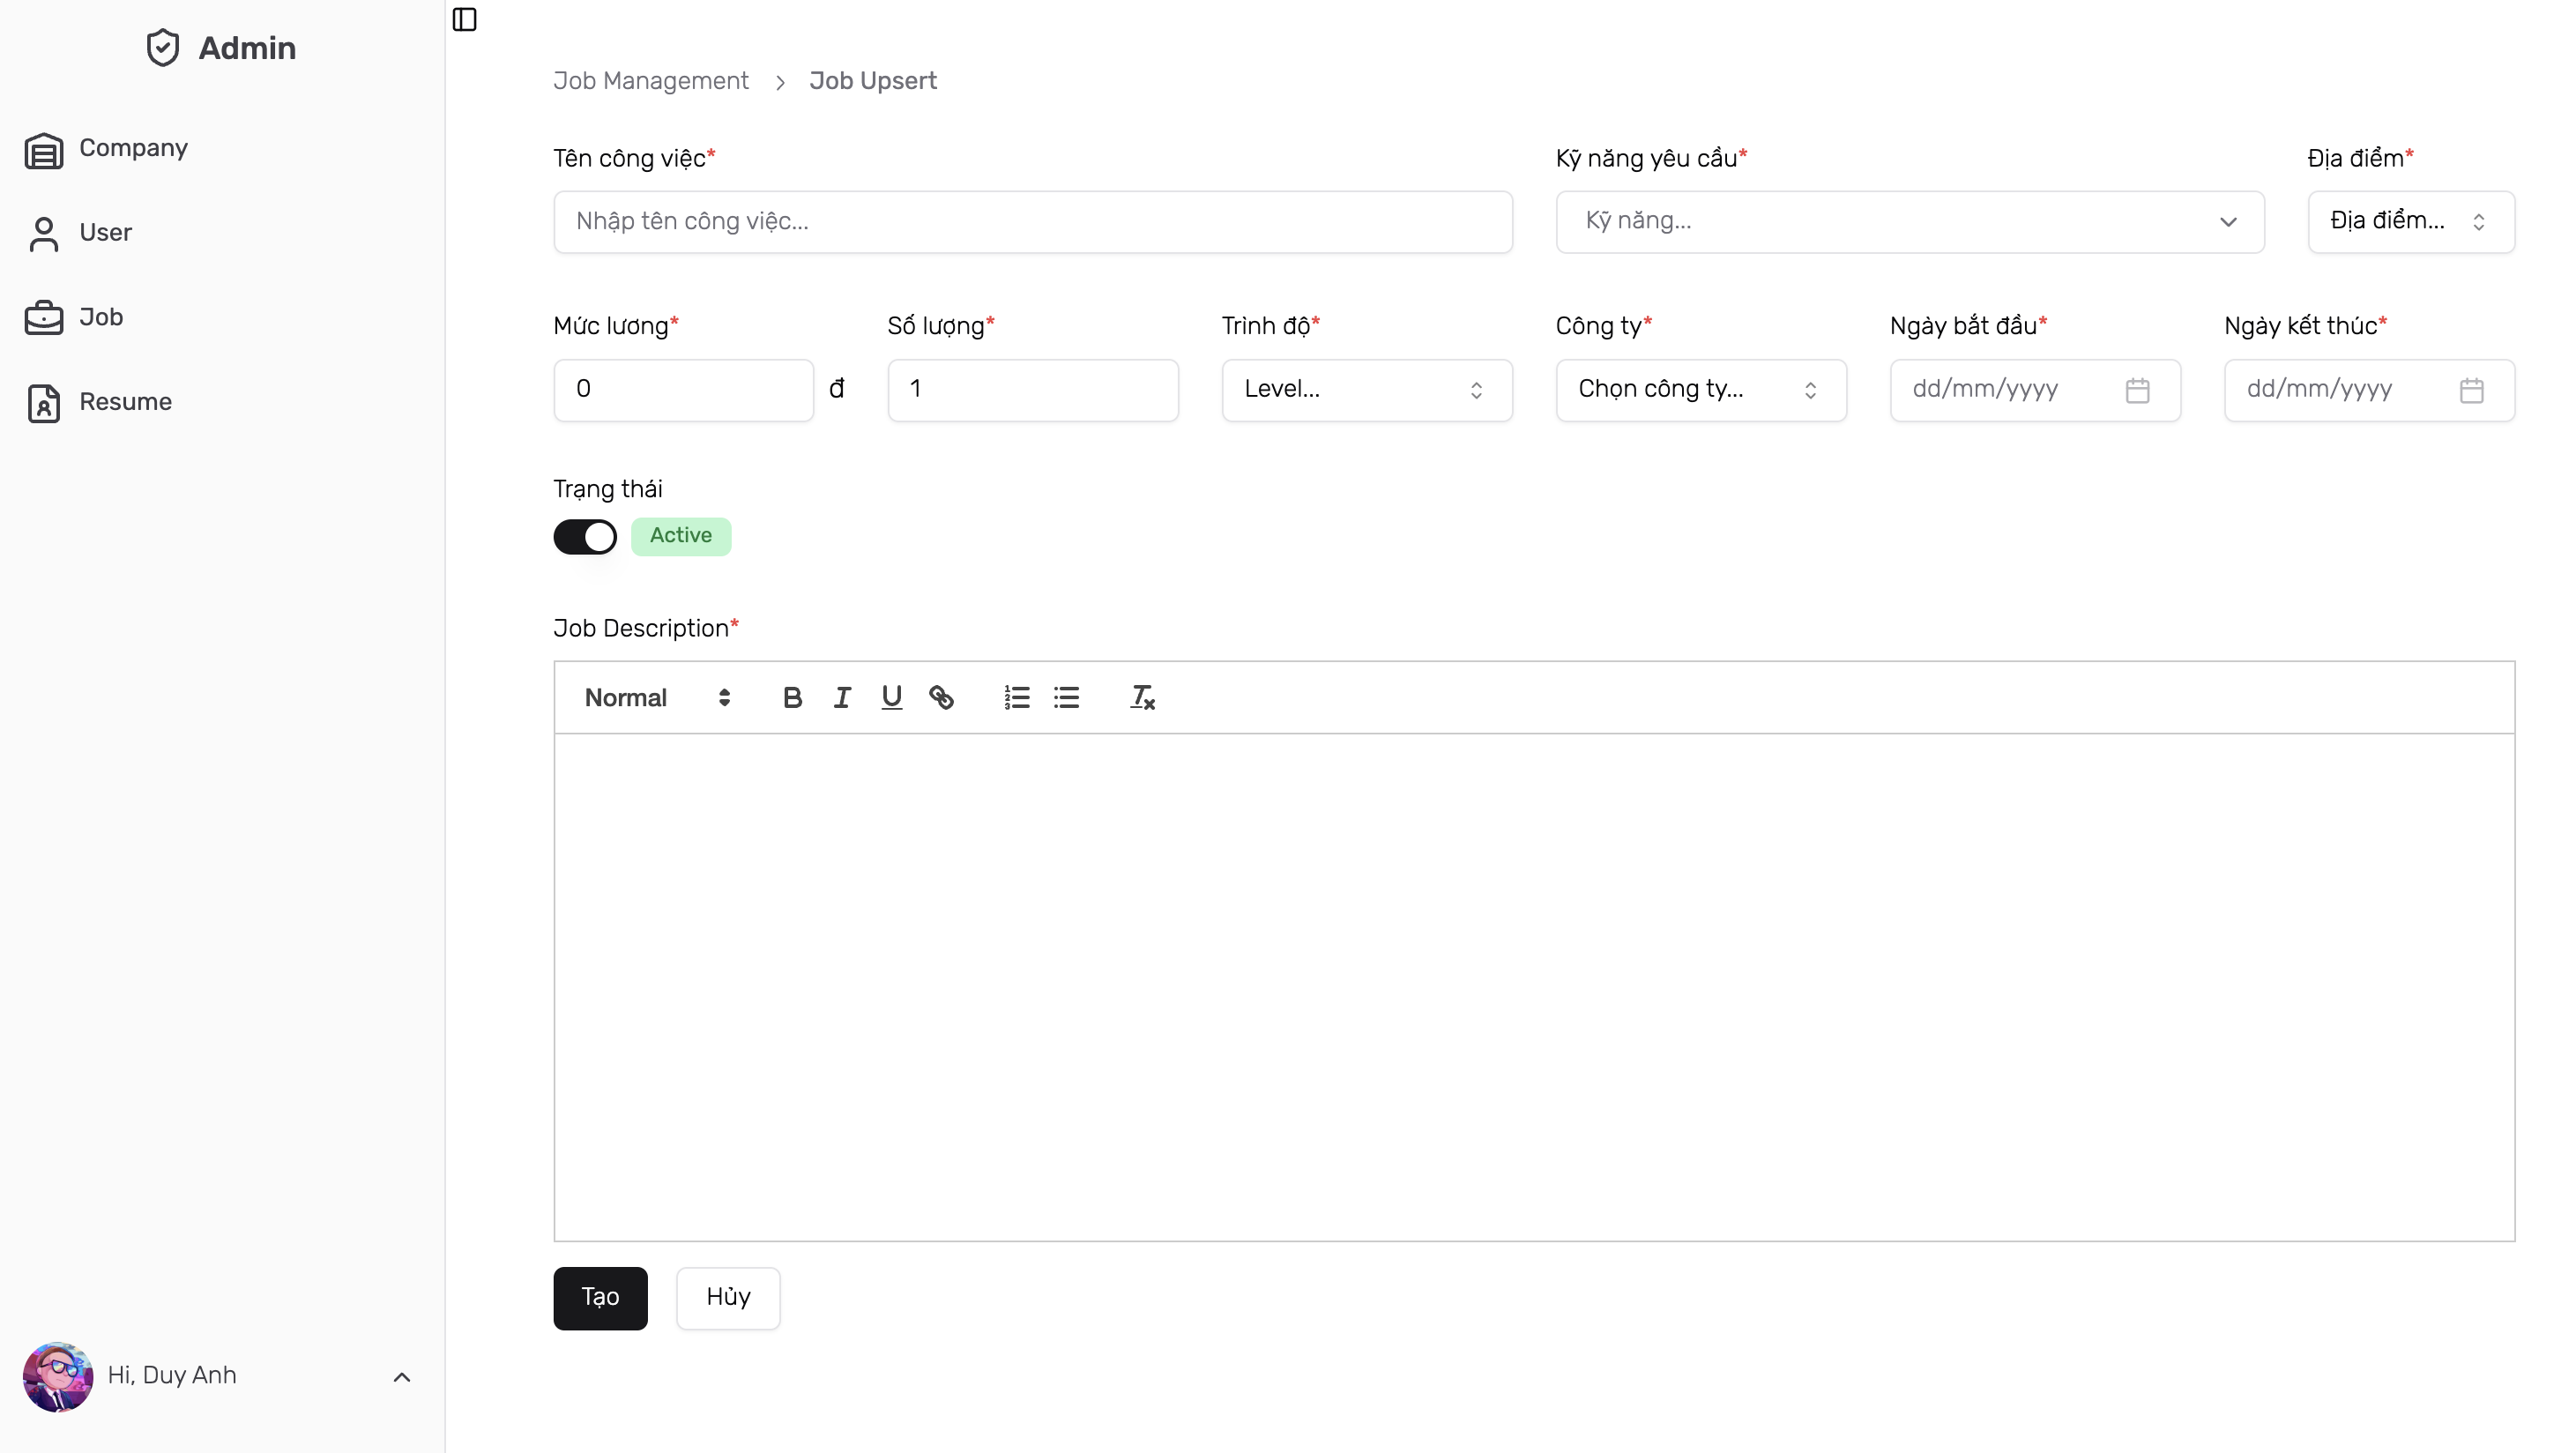
\includegraphics[width=\linewidth]{DBMS-Application/Images/create-job.png}
    \caption{Trang quản lý công việc - Thêm công việc mới}
    \label{fig:enter-label}
\end{figure}

Truy vấn sử dụng: \textbf{Insert}

\begin{lstlisting}
async create(createJobDto: CreateJobDto) {
    const job = {
      ...createJobDto,
      createdAt: new Date(),
      updatedAt: new Date(),
    };

    const result = await this.db.collection('jobs').insertOne(job); // Insert cong viec moi vao collection 'jobs'
    return { _id: result.insertedId, createdAt: job.createdAt };
}
\end{lstlisting}

Quản trị viên cũng có thể chọn một công việc để chỉnh sửa/cập nhật thông tin. Khi đó, dựa vào \texttt{\_id}, hệ thống sẽ truy vấn cơ sở dữ liệu để lấy ra công việc đó (\textbf{query with single condition}) và hiển thị lên giao diện. Lúc này, quản trị viên có thể tiến hành sửa lại các thông tin đó và khi hoàn tất, Front-end sẽ gửi yêu cầu qua API với phương thức HTTP \textbf{PATCH} để hệ thống tiến hành cập nhật lại thông tin cho công việc đó trong cơ sở dữ liệu.

\begin{figure}[H]
    \centering
    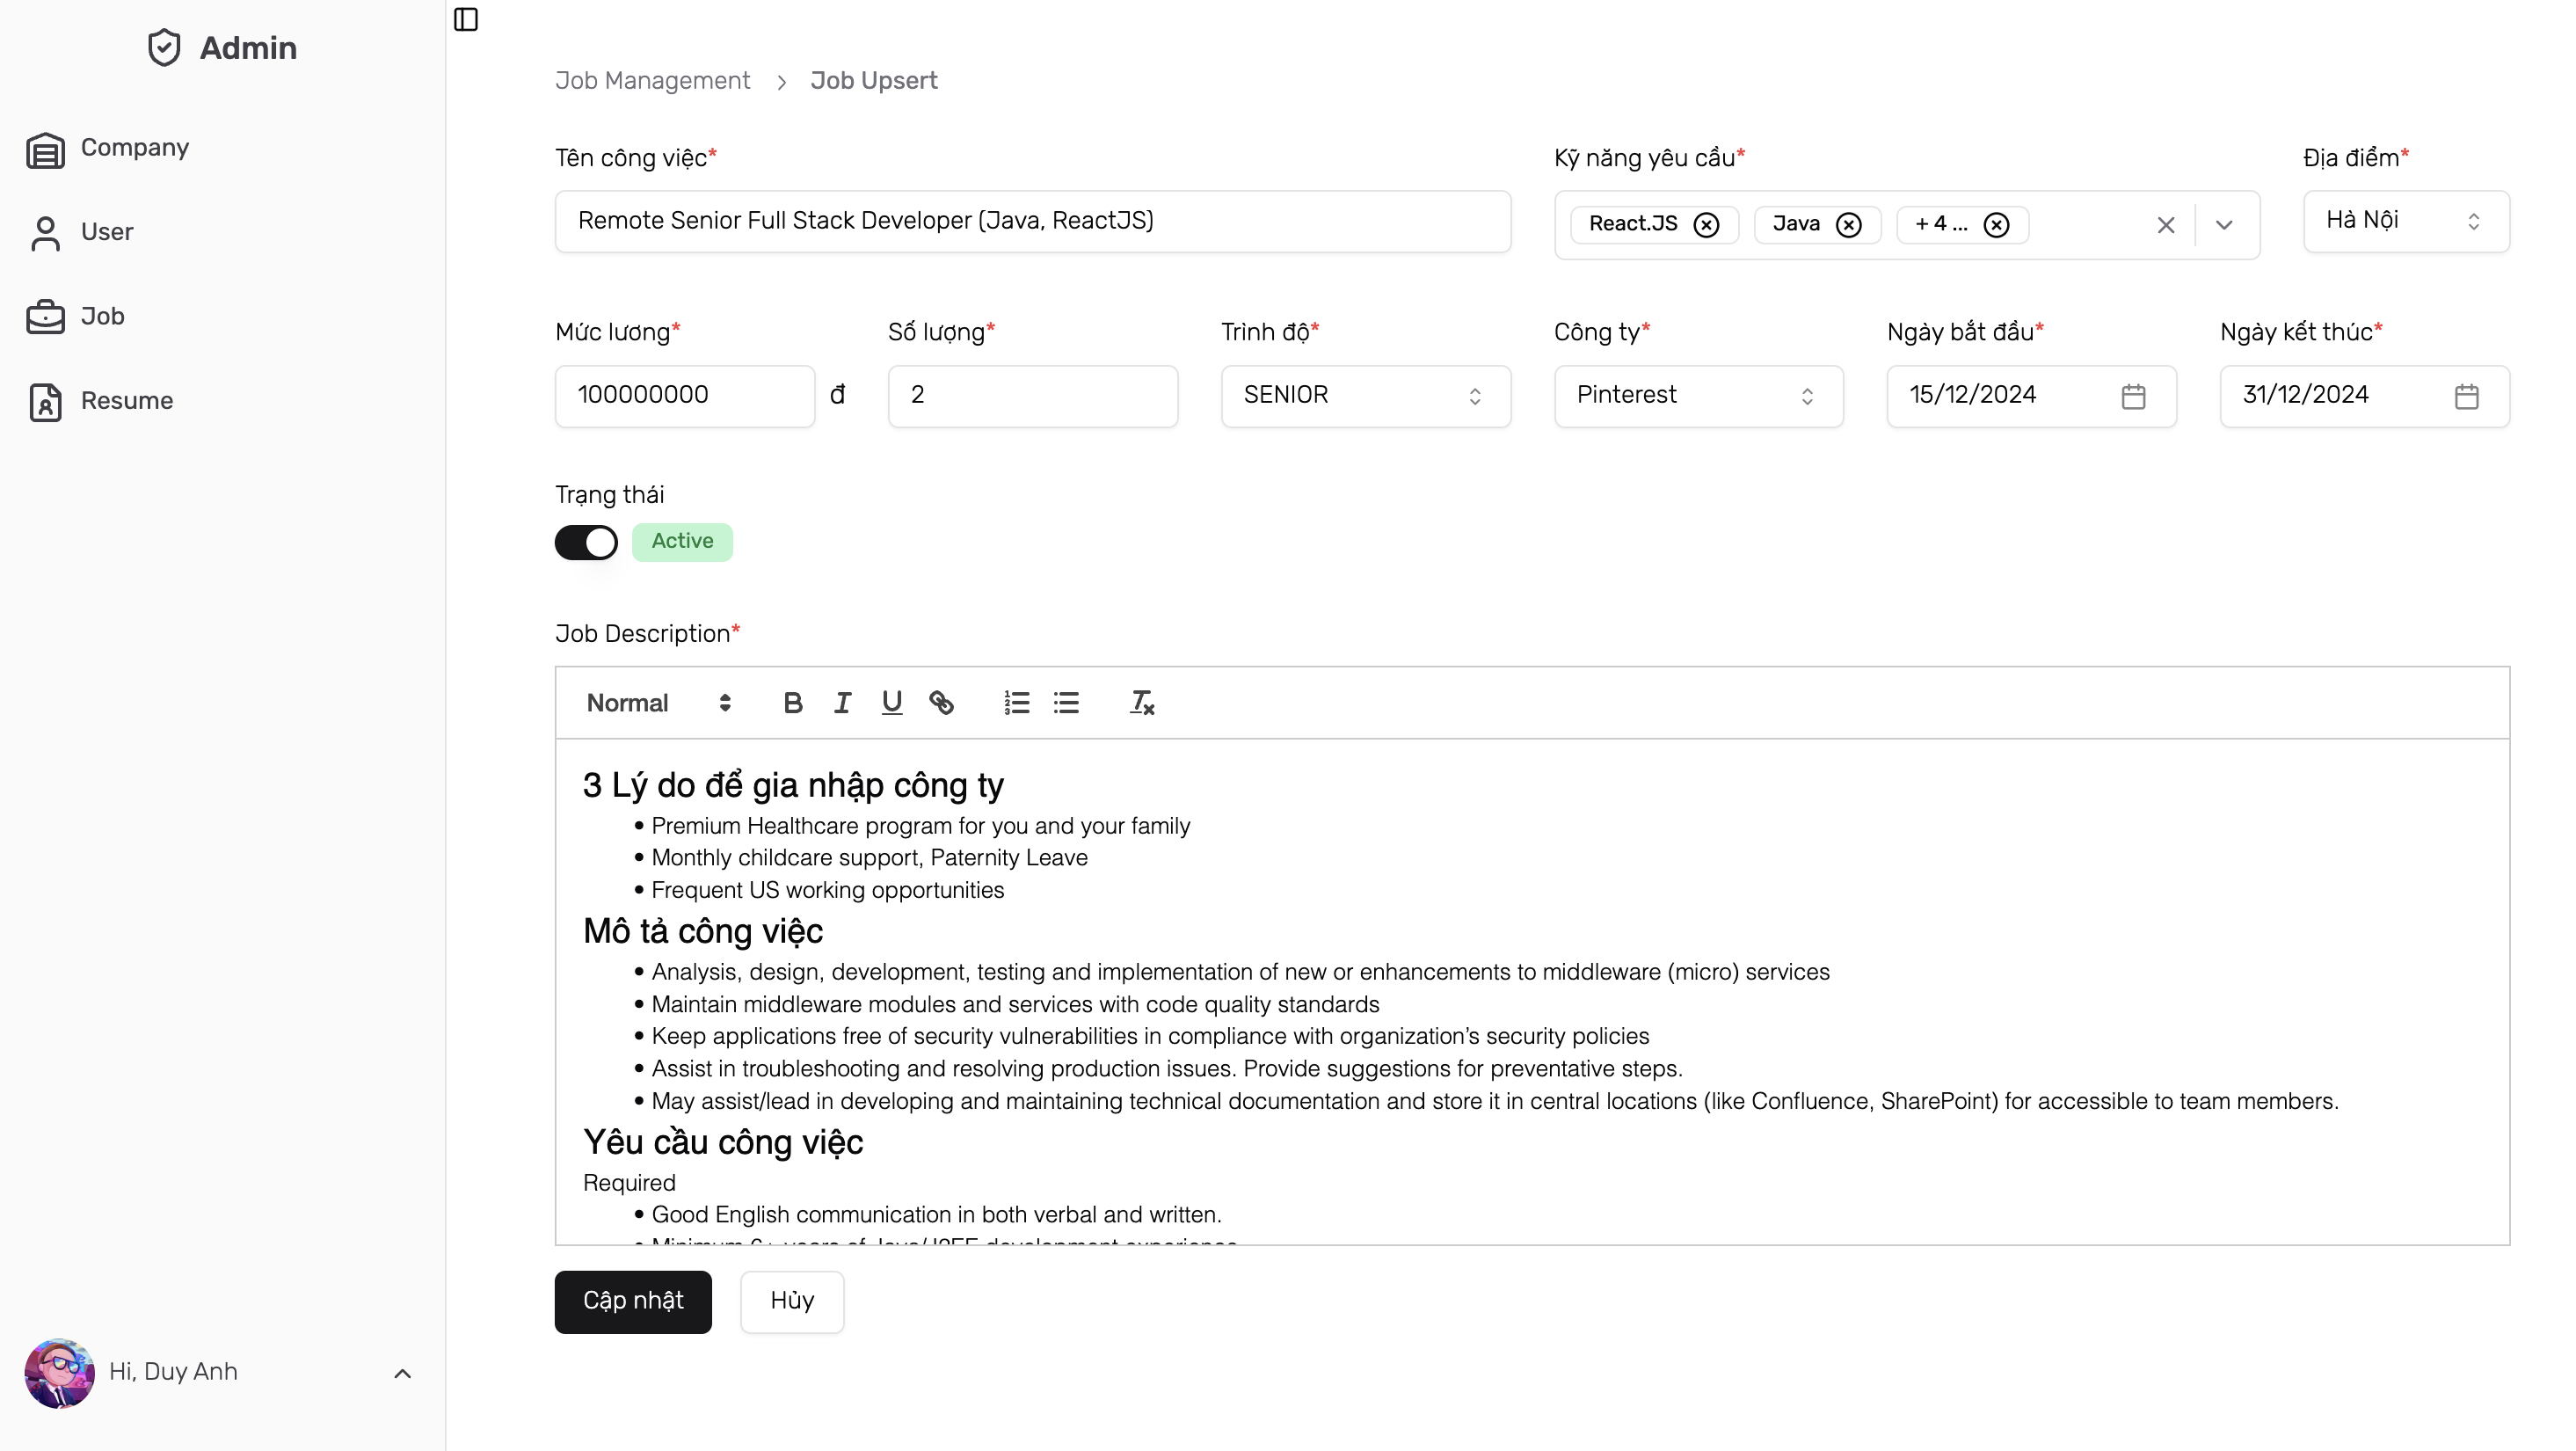
\includegraphics[width=\linewidth]{DBMS-Application/Images/update-job.png}
    \caption{Trang quản lý công việc - Cập nhật thông tin cho một công việc cụ thể}
    \label{fig:enter-label}
\end{figure}

Truy vấn sử dụng: \textbf{Update}

\begin{lstlisting}
const result = await this.db.collection('jobs').updateOne(
  { _id: new ObjectId(id) },
  {
    $set: {
      ...updateJobDto,
      updatedAt: new Date(),
    },
  },
);
\end{lstlisting}

Cuối cùng, quản trị viên có thể chọn một công việc để xoá khỏi hệ thống. Khi đó, một popup sẽ hiện lên để xác nhận với quản trị viên về việc xoá công ty đã chọn ra khỏi cơ sở dữ liệu

\begin{figure}[H]
    \centering
    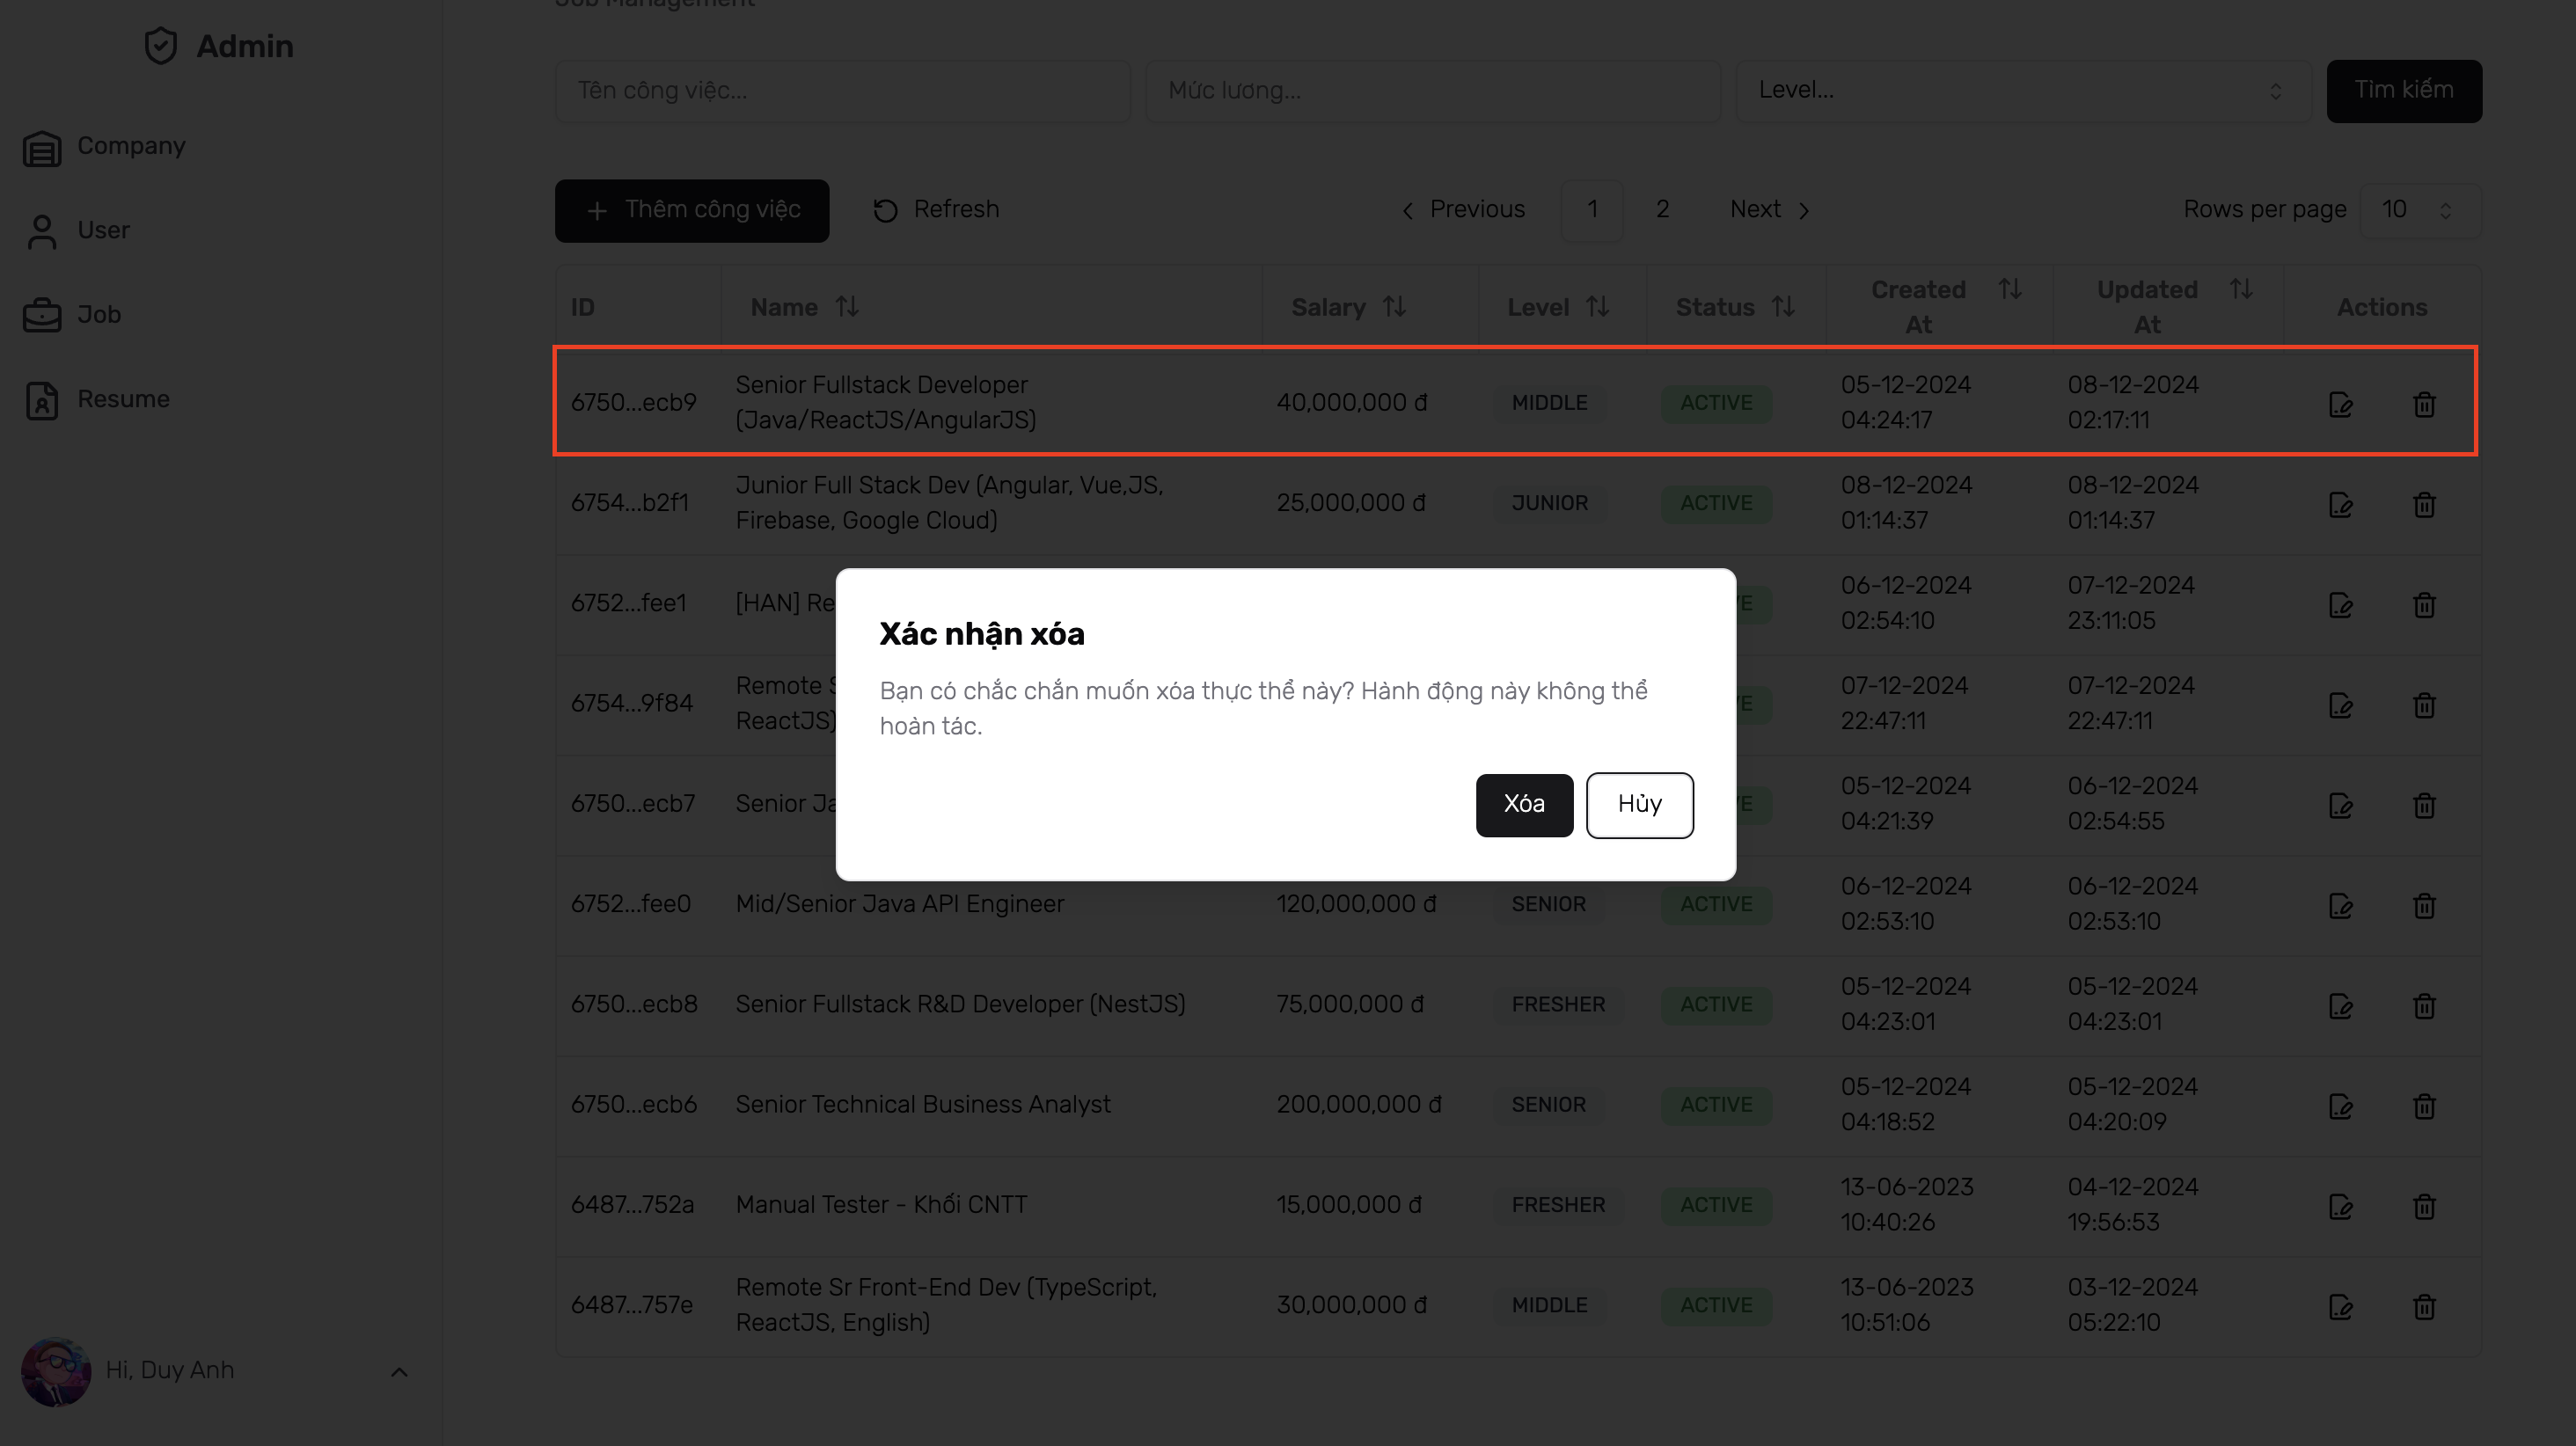
\includegraphics[width=\linewidth]{DBMS-Application/Images/delete-job.png}
    \caption{Trang quản lý công việc - Xác nhận xoá công việc chỉ định khỏi hệ thống}
    \label{fig:enter-label}
\end{figure}

Khi quản trị viên xác nhận, Back-end gửi truy vấn đến cơ sở dữ liệu để tìm theo \texttt{\_id} và xoá công việc đó ra khỏi cơ sở dữ liệu. Khi đó, giao diện người dùng sẽ được cập nhật lại.\\

\begin{figure}[H]
    \centering
    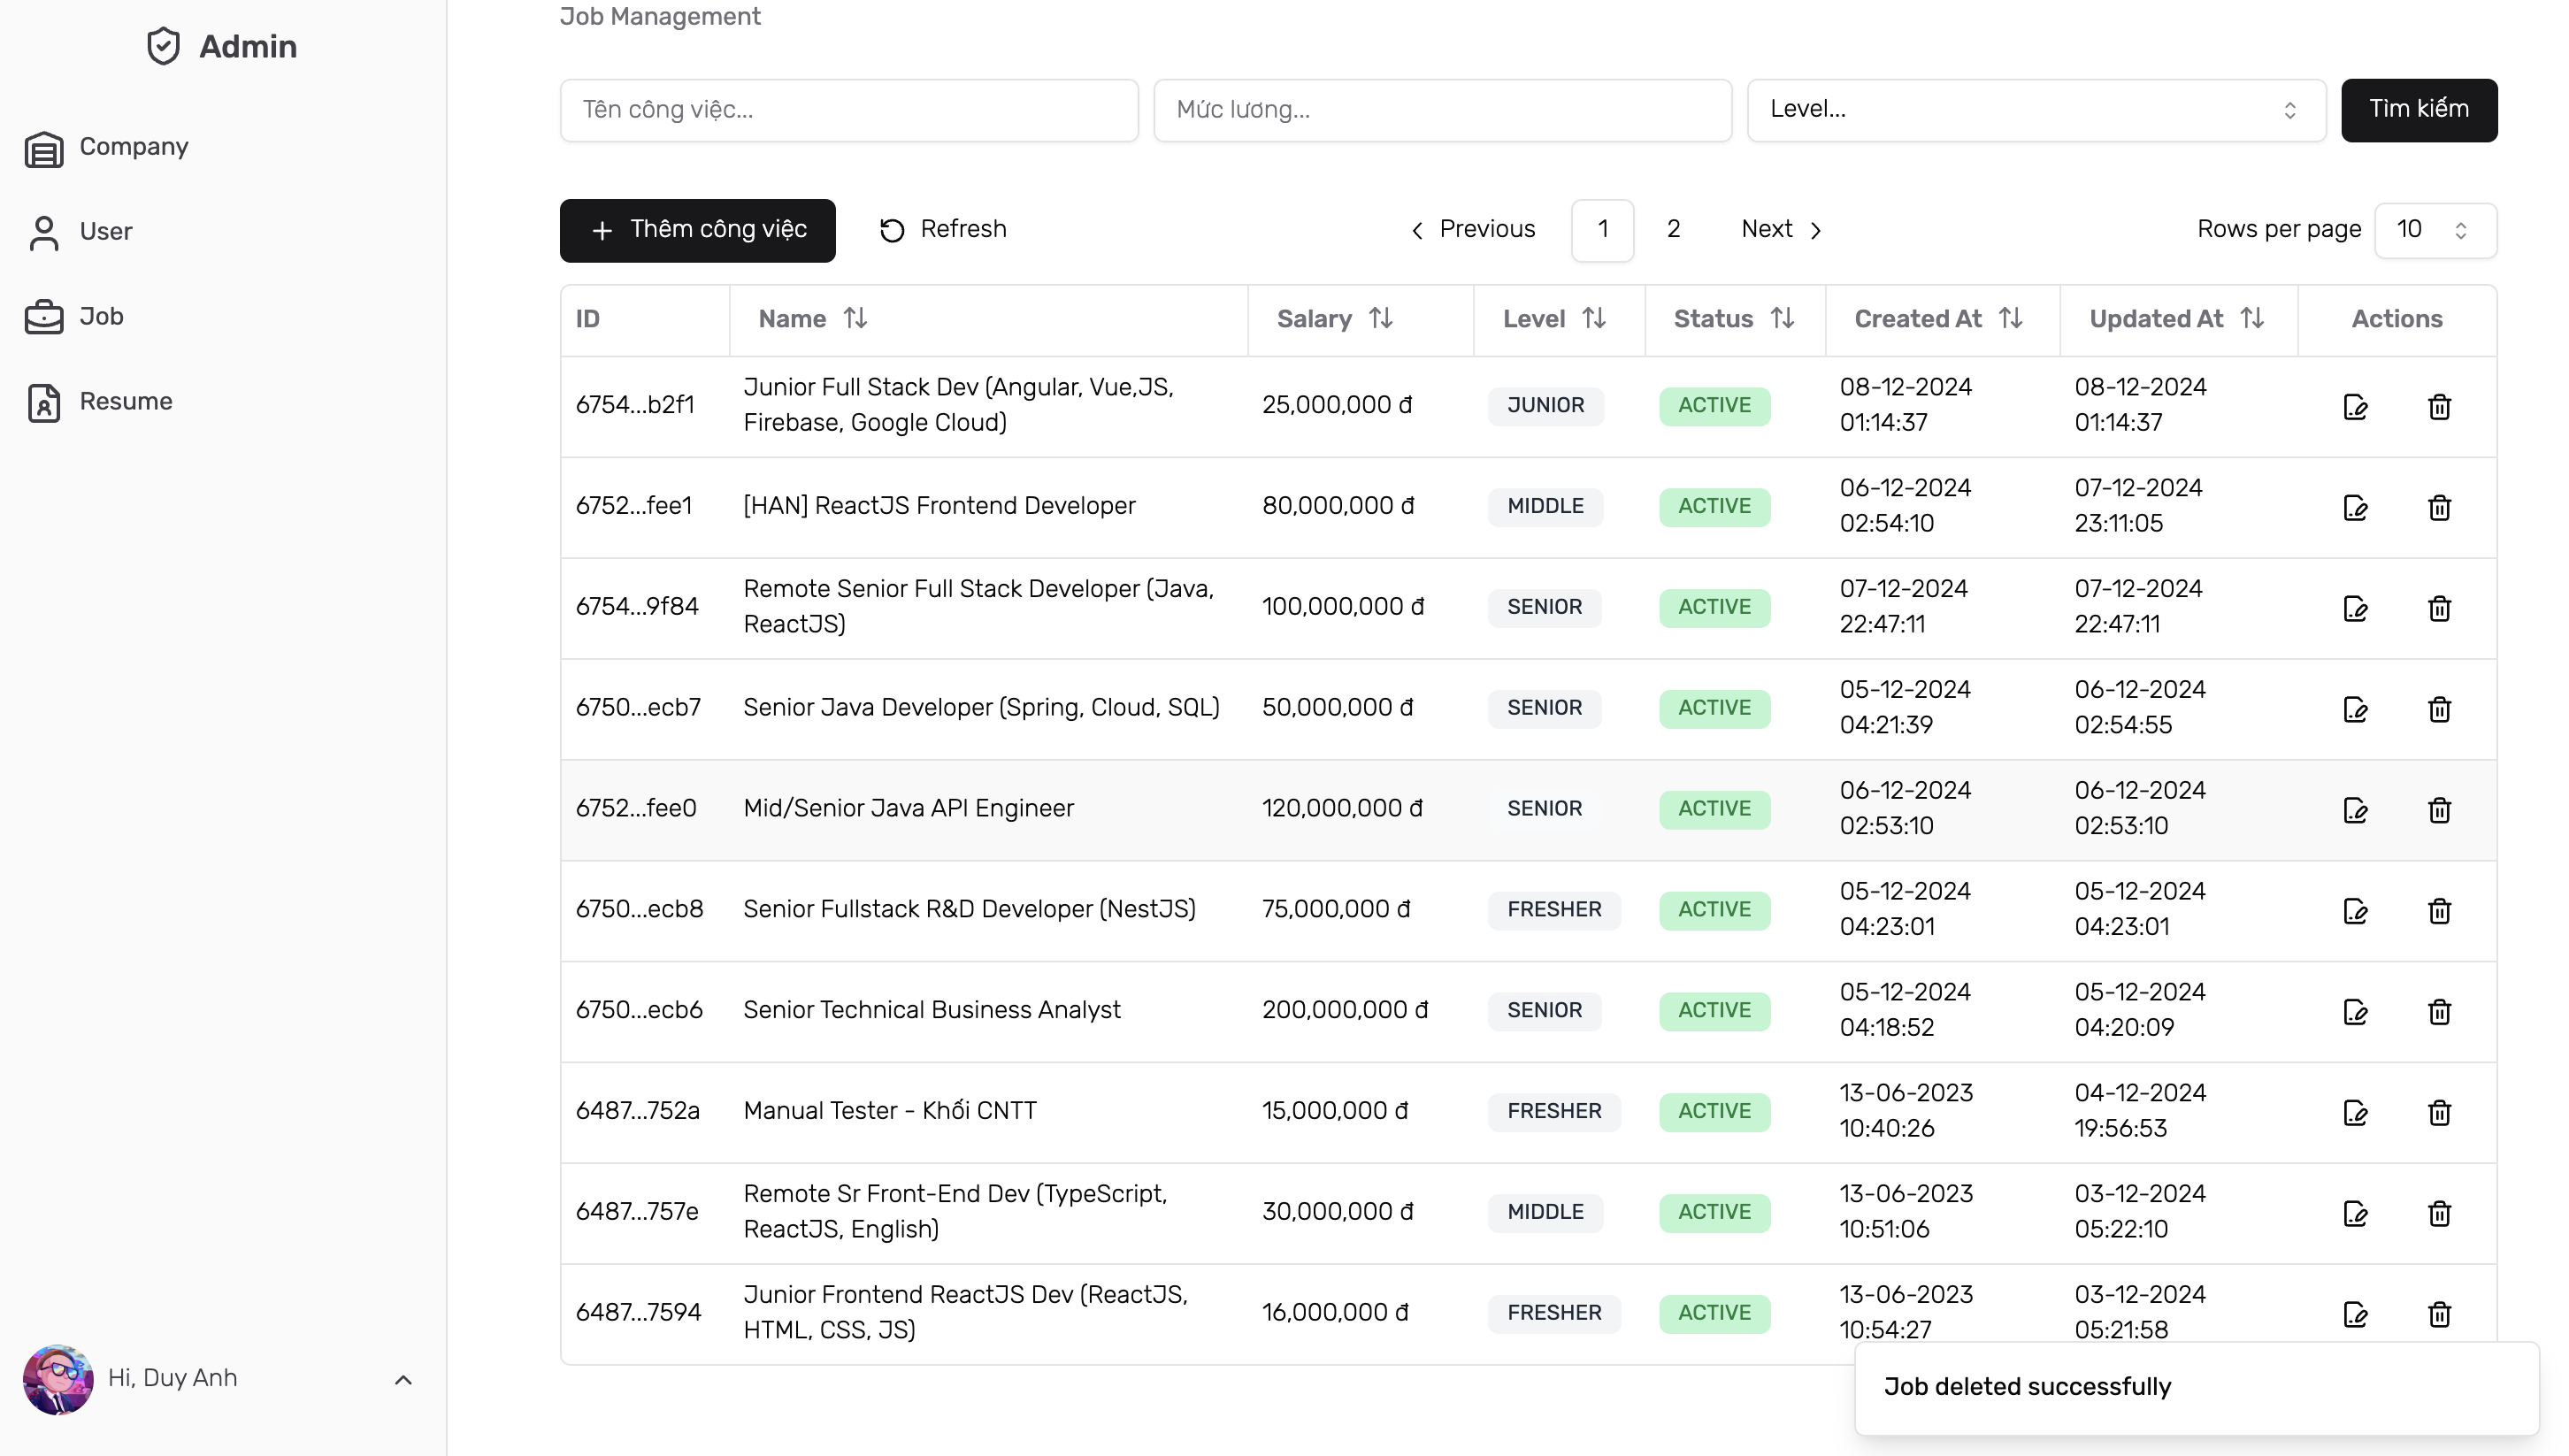
\includegraphics[width=\linewidth]{DBMS-Application/Images/delete-job-successfully.png}
    \caption{Trang quản lý công việc - Xoá thành công công việc đã chọn}
    \label{fig:enter-label}
\end{figure}

Truy vấn sử dụng: \textbf{Delete}

\begin{lstlisting}
const result = await this.db
      .collection('jobs')
      .deleteOne({ _id: new ObjectId(id) });
\end{lstlisting}

% \subsubsection{Giao diện Admin - Quản lý công ty}

Tương tự trang quản lý công việc, trang quản lý công ty cũng sử dụng các loại truy vấn sau để hỗ trợ cho các thao tác CRUD:
\begin{itemize}
    \item \textbf{Query with single/composite condition}: Để fetch lên dữ liệu toàn bộ công ty trong hệ thống theo cơ chế phân trang và một số điều kiện như \textbf{Tên công ty}, \textbf{Địa chỉ}
    \begin{figure}[H]
        \centering
        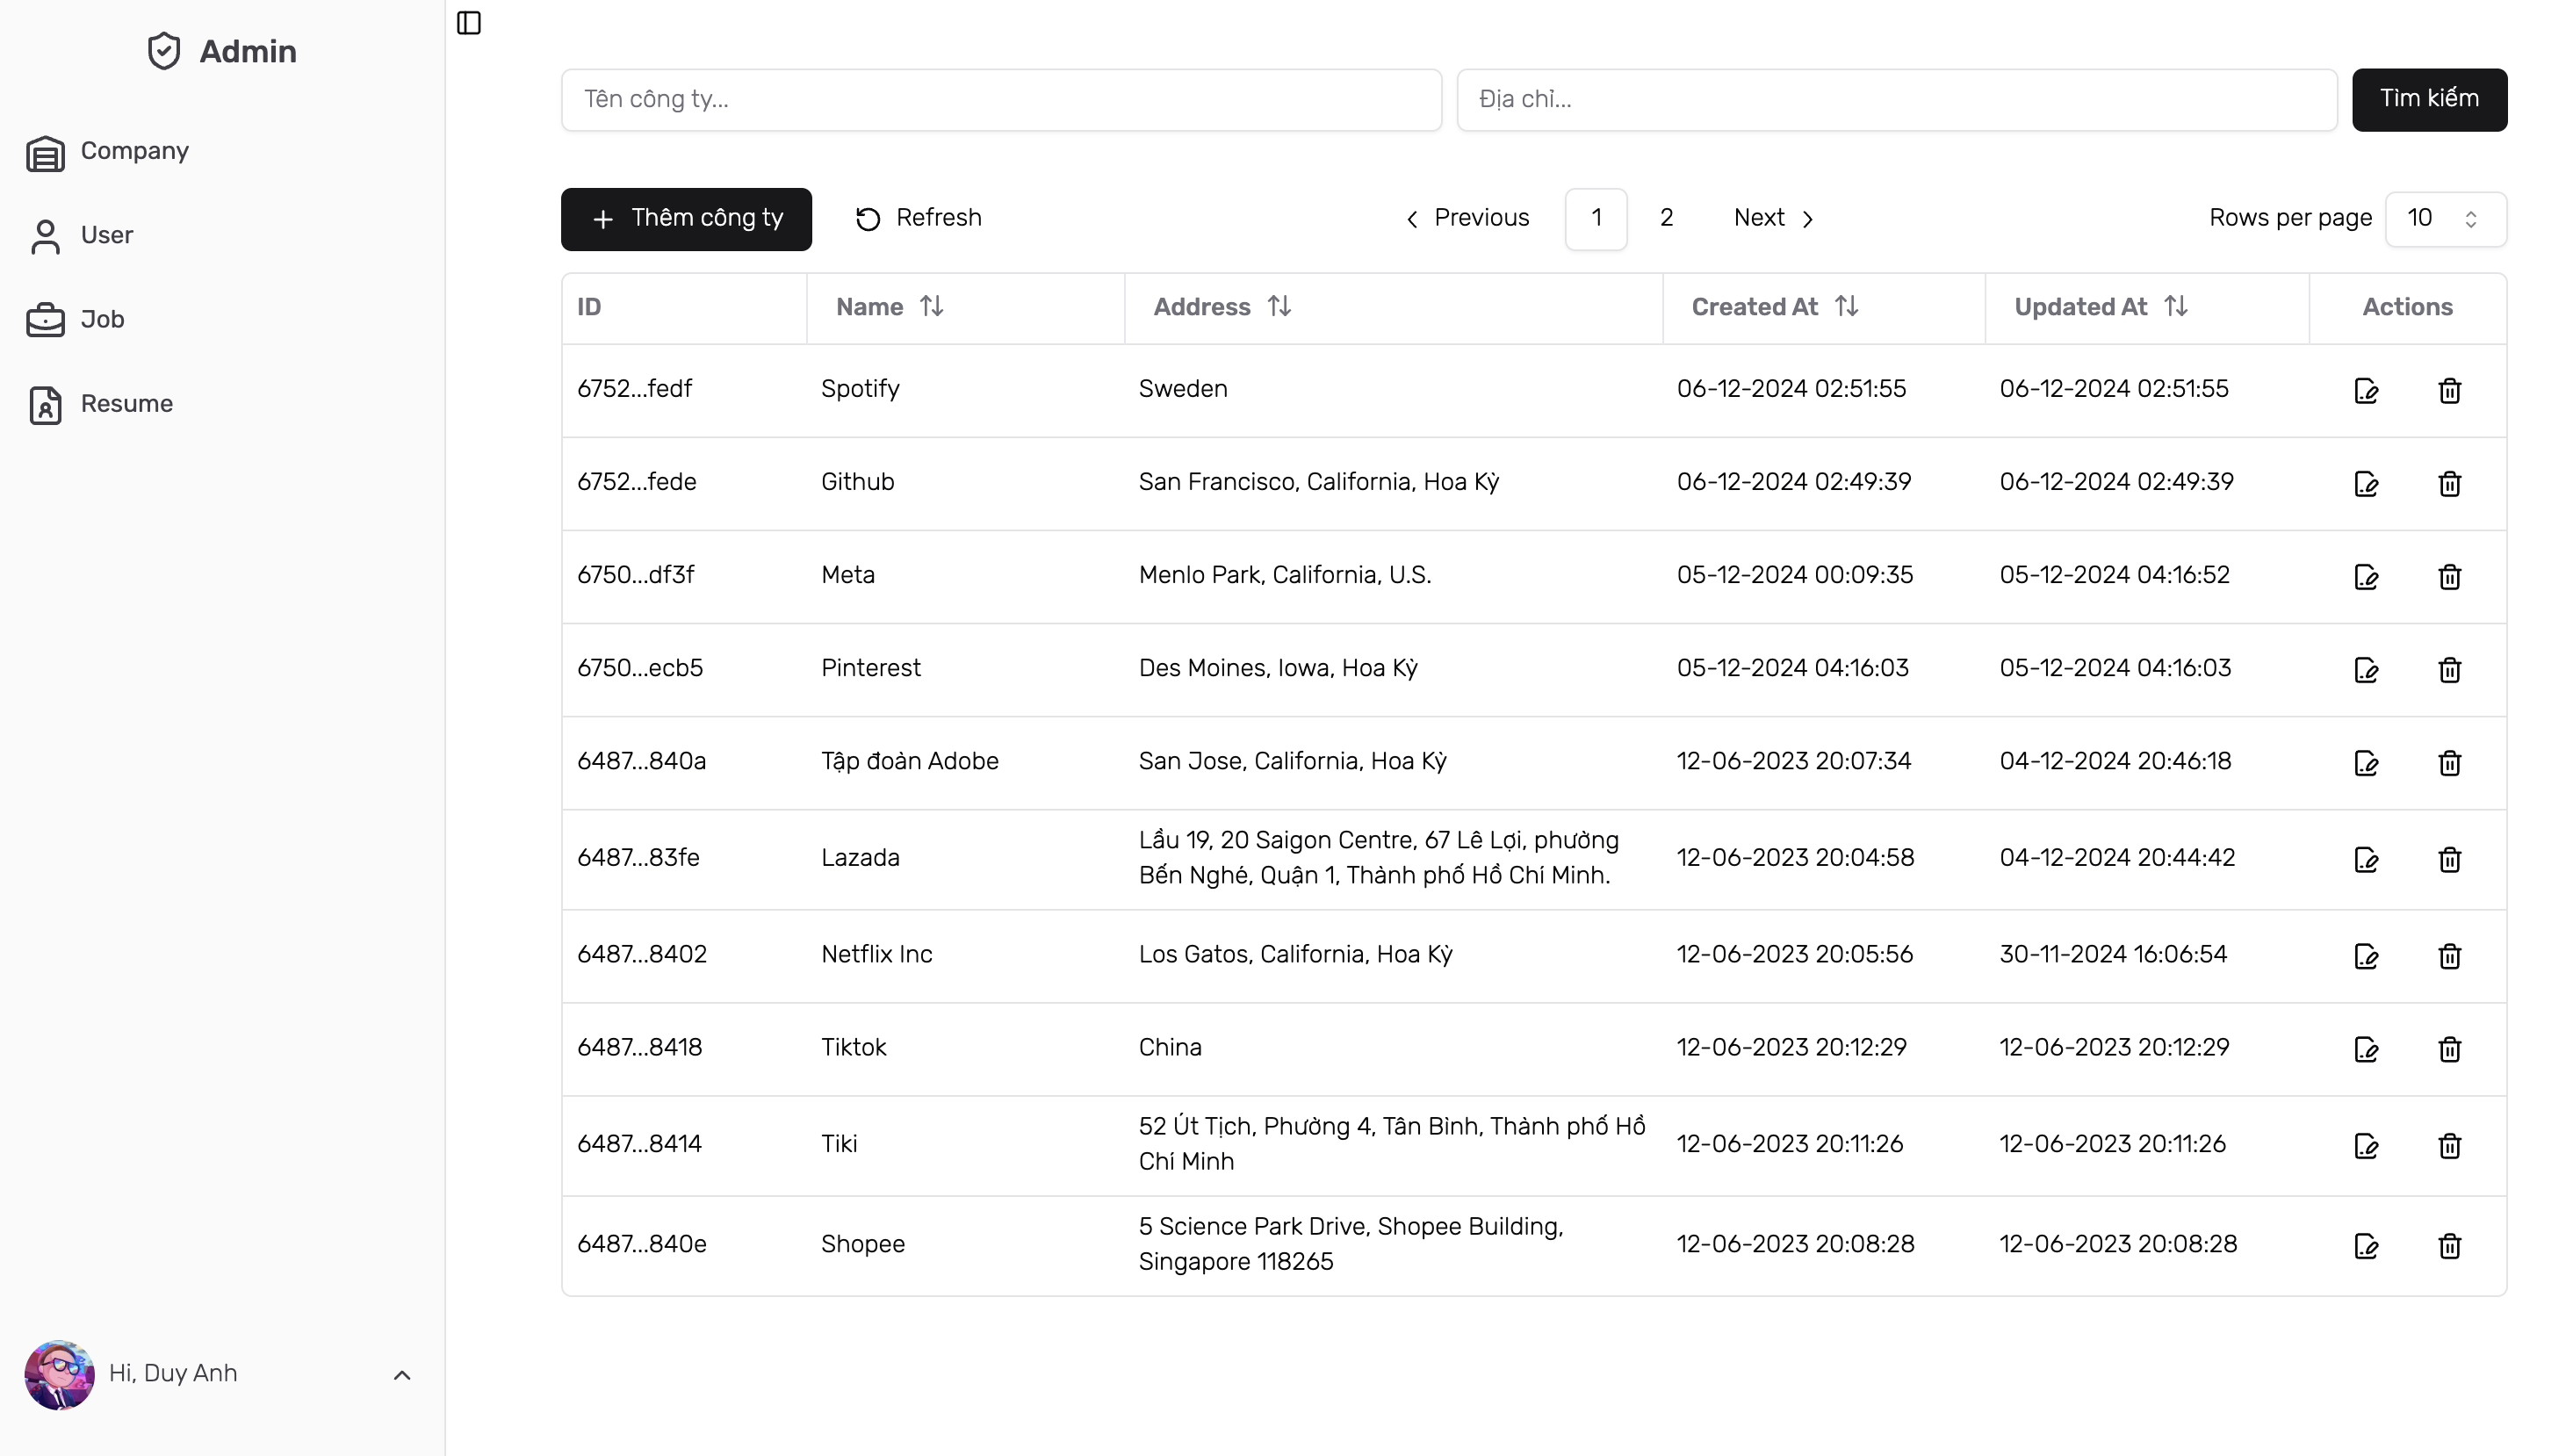
\includegraphics[width=\linewidth]{DBMS-Application/Images/admin-company.png}
        \caption{Trang quản lý công ty - Danh sách các công ty trong hệ thống}
        \label{fig:enter-label}
    \end{figure}

    \begin{figure}[H]
        \centering
        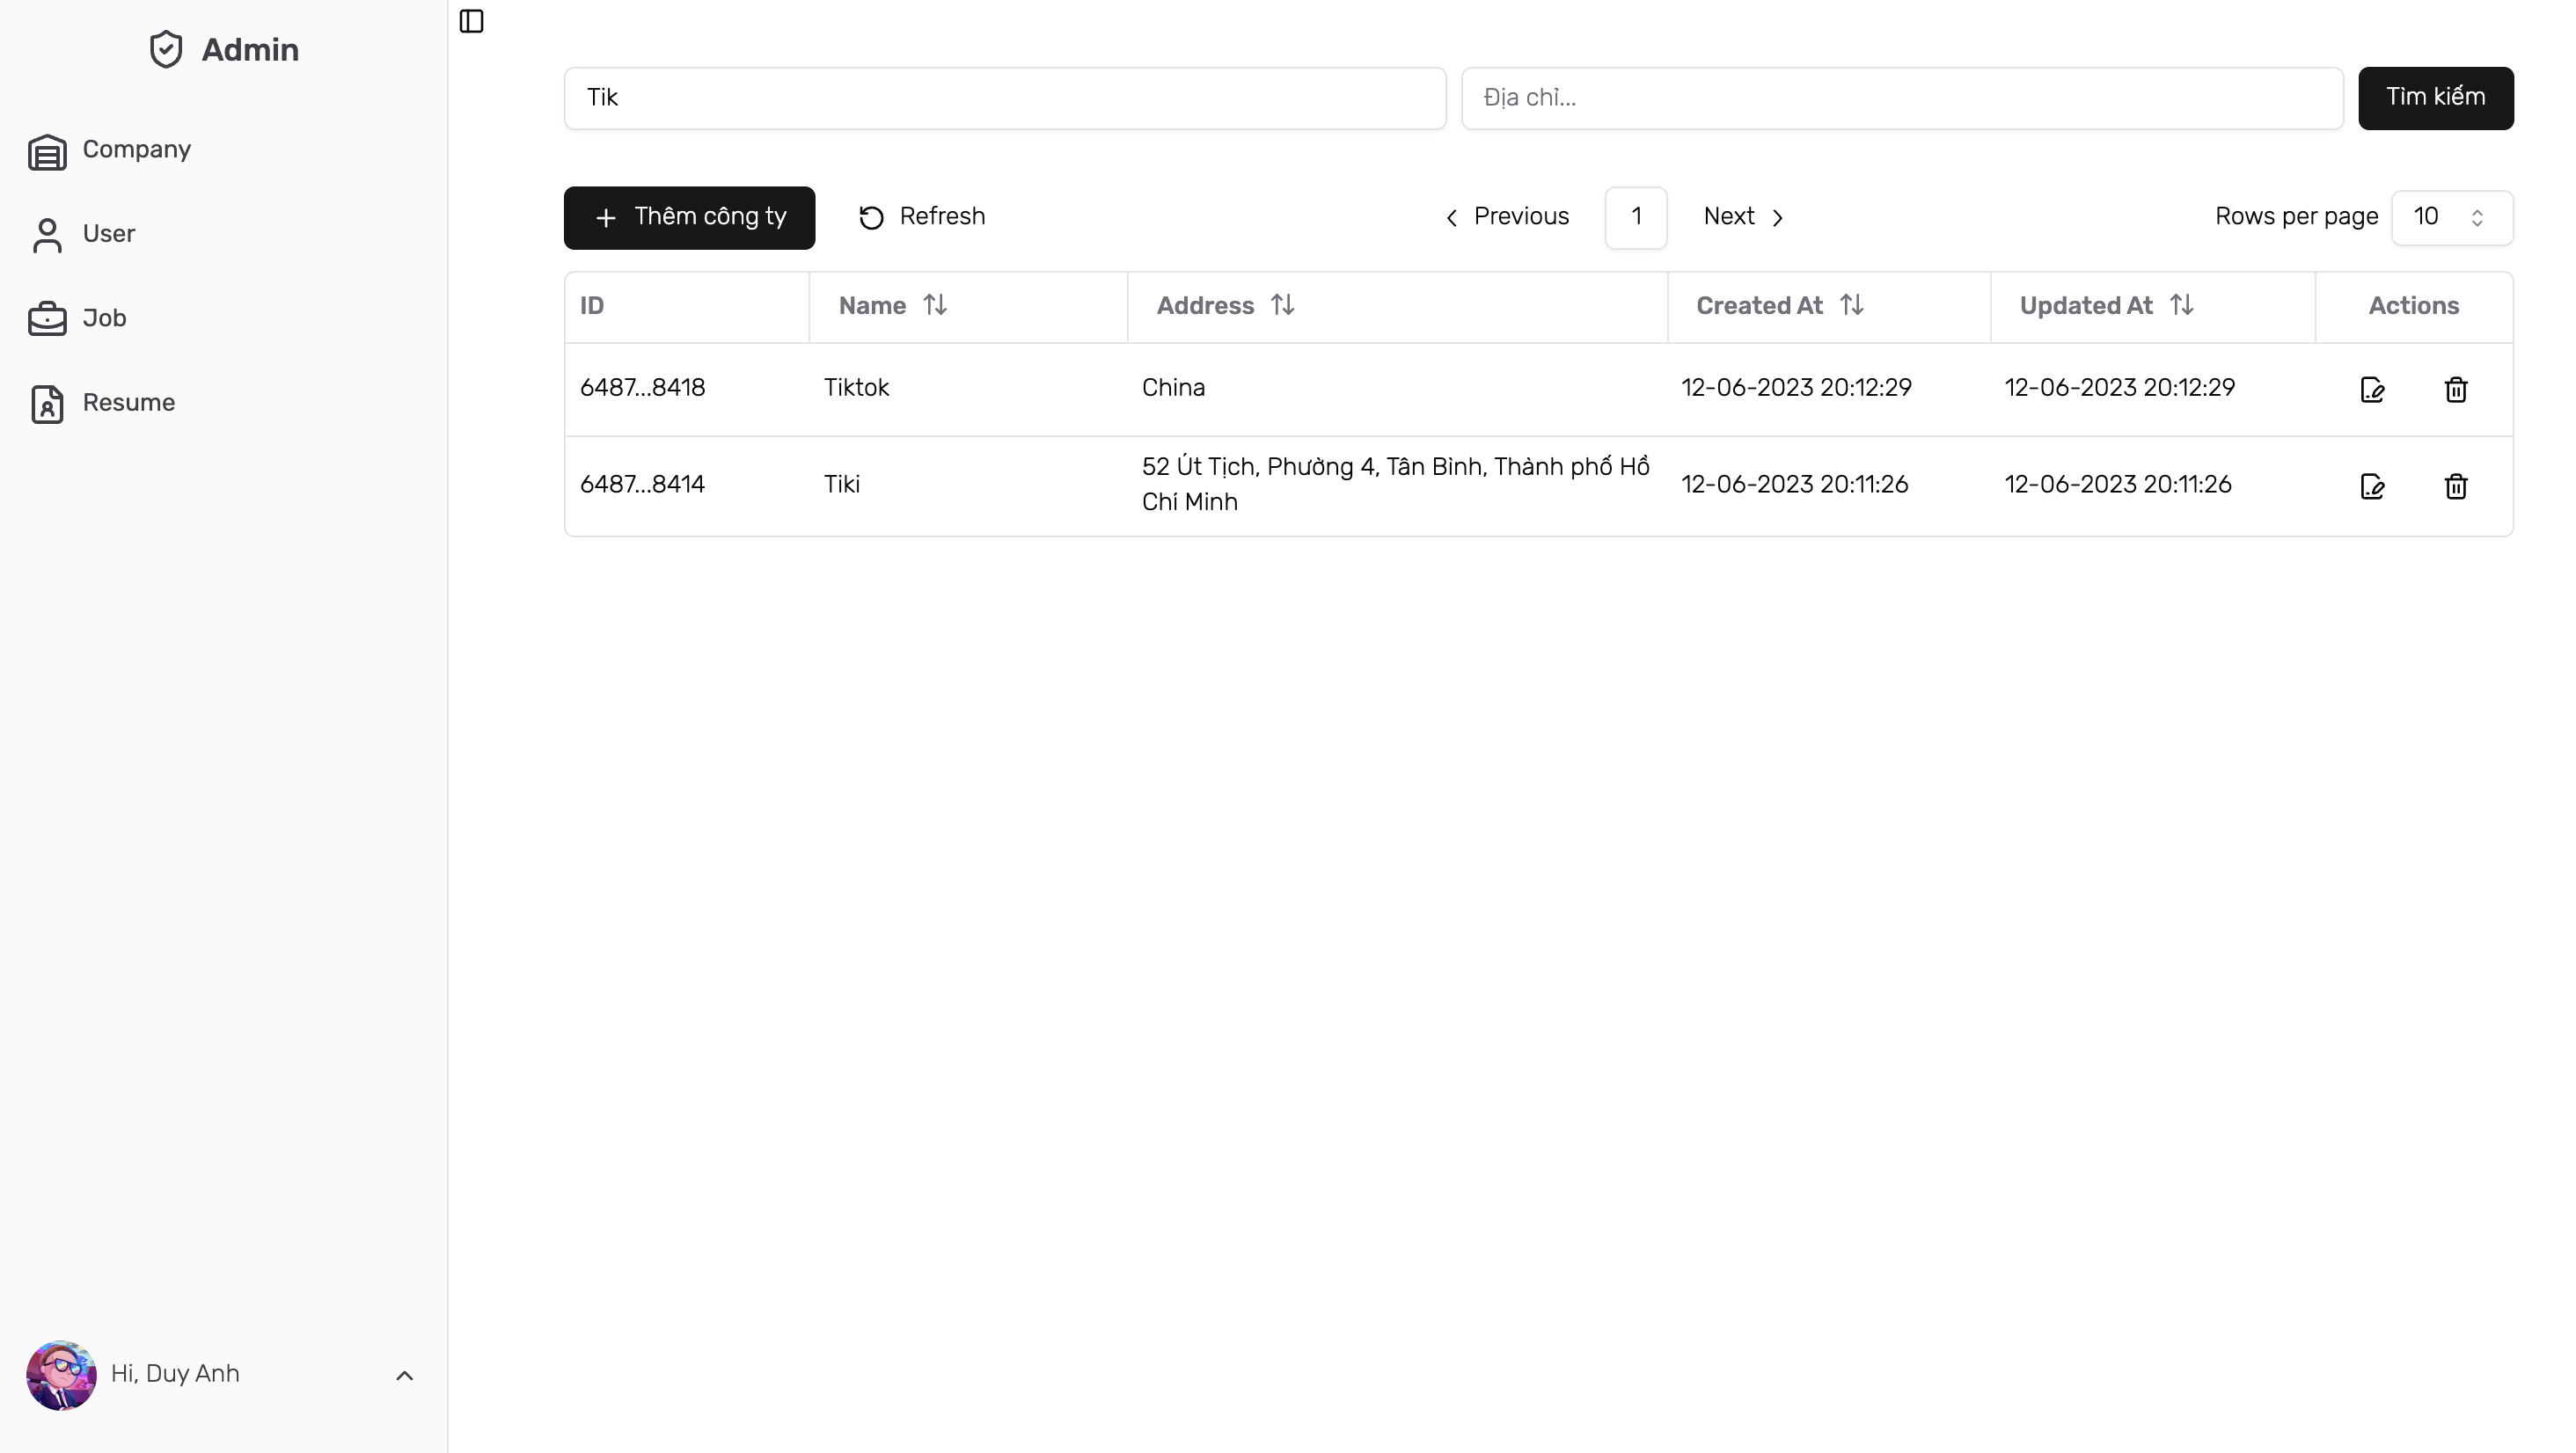
\includegraphics[width=\linewidth]{DBMS-Application/Images/admin-company-filter.png}
        \caption{Trang quản lý công ty - Danh sách công ty lọc theo điều kiện}
        \label{fig:enter-label}
    \end{figure}
    
    \item \textbf{Insert}: Thêm mới một công ty
    \begin{figure}[H]
        \centering
        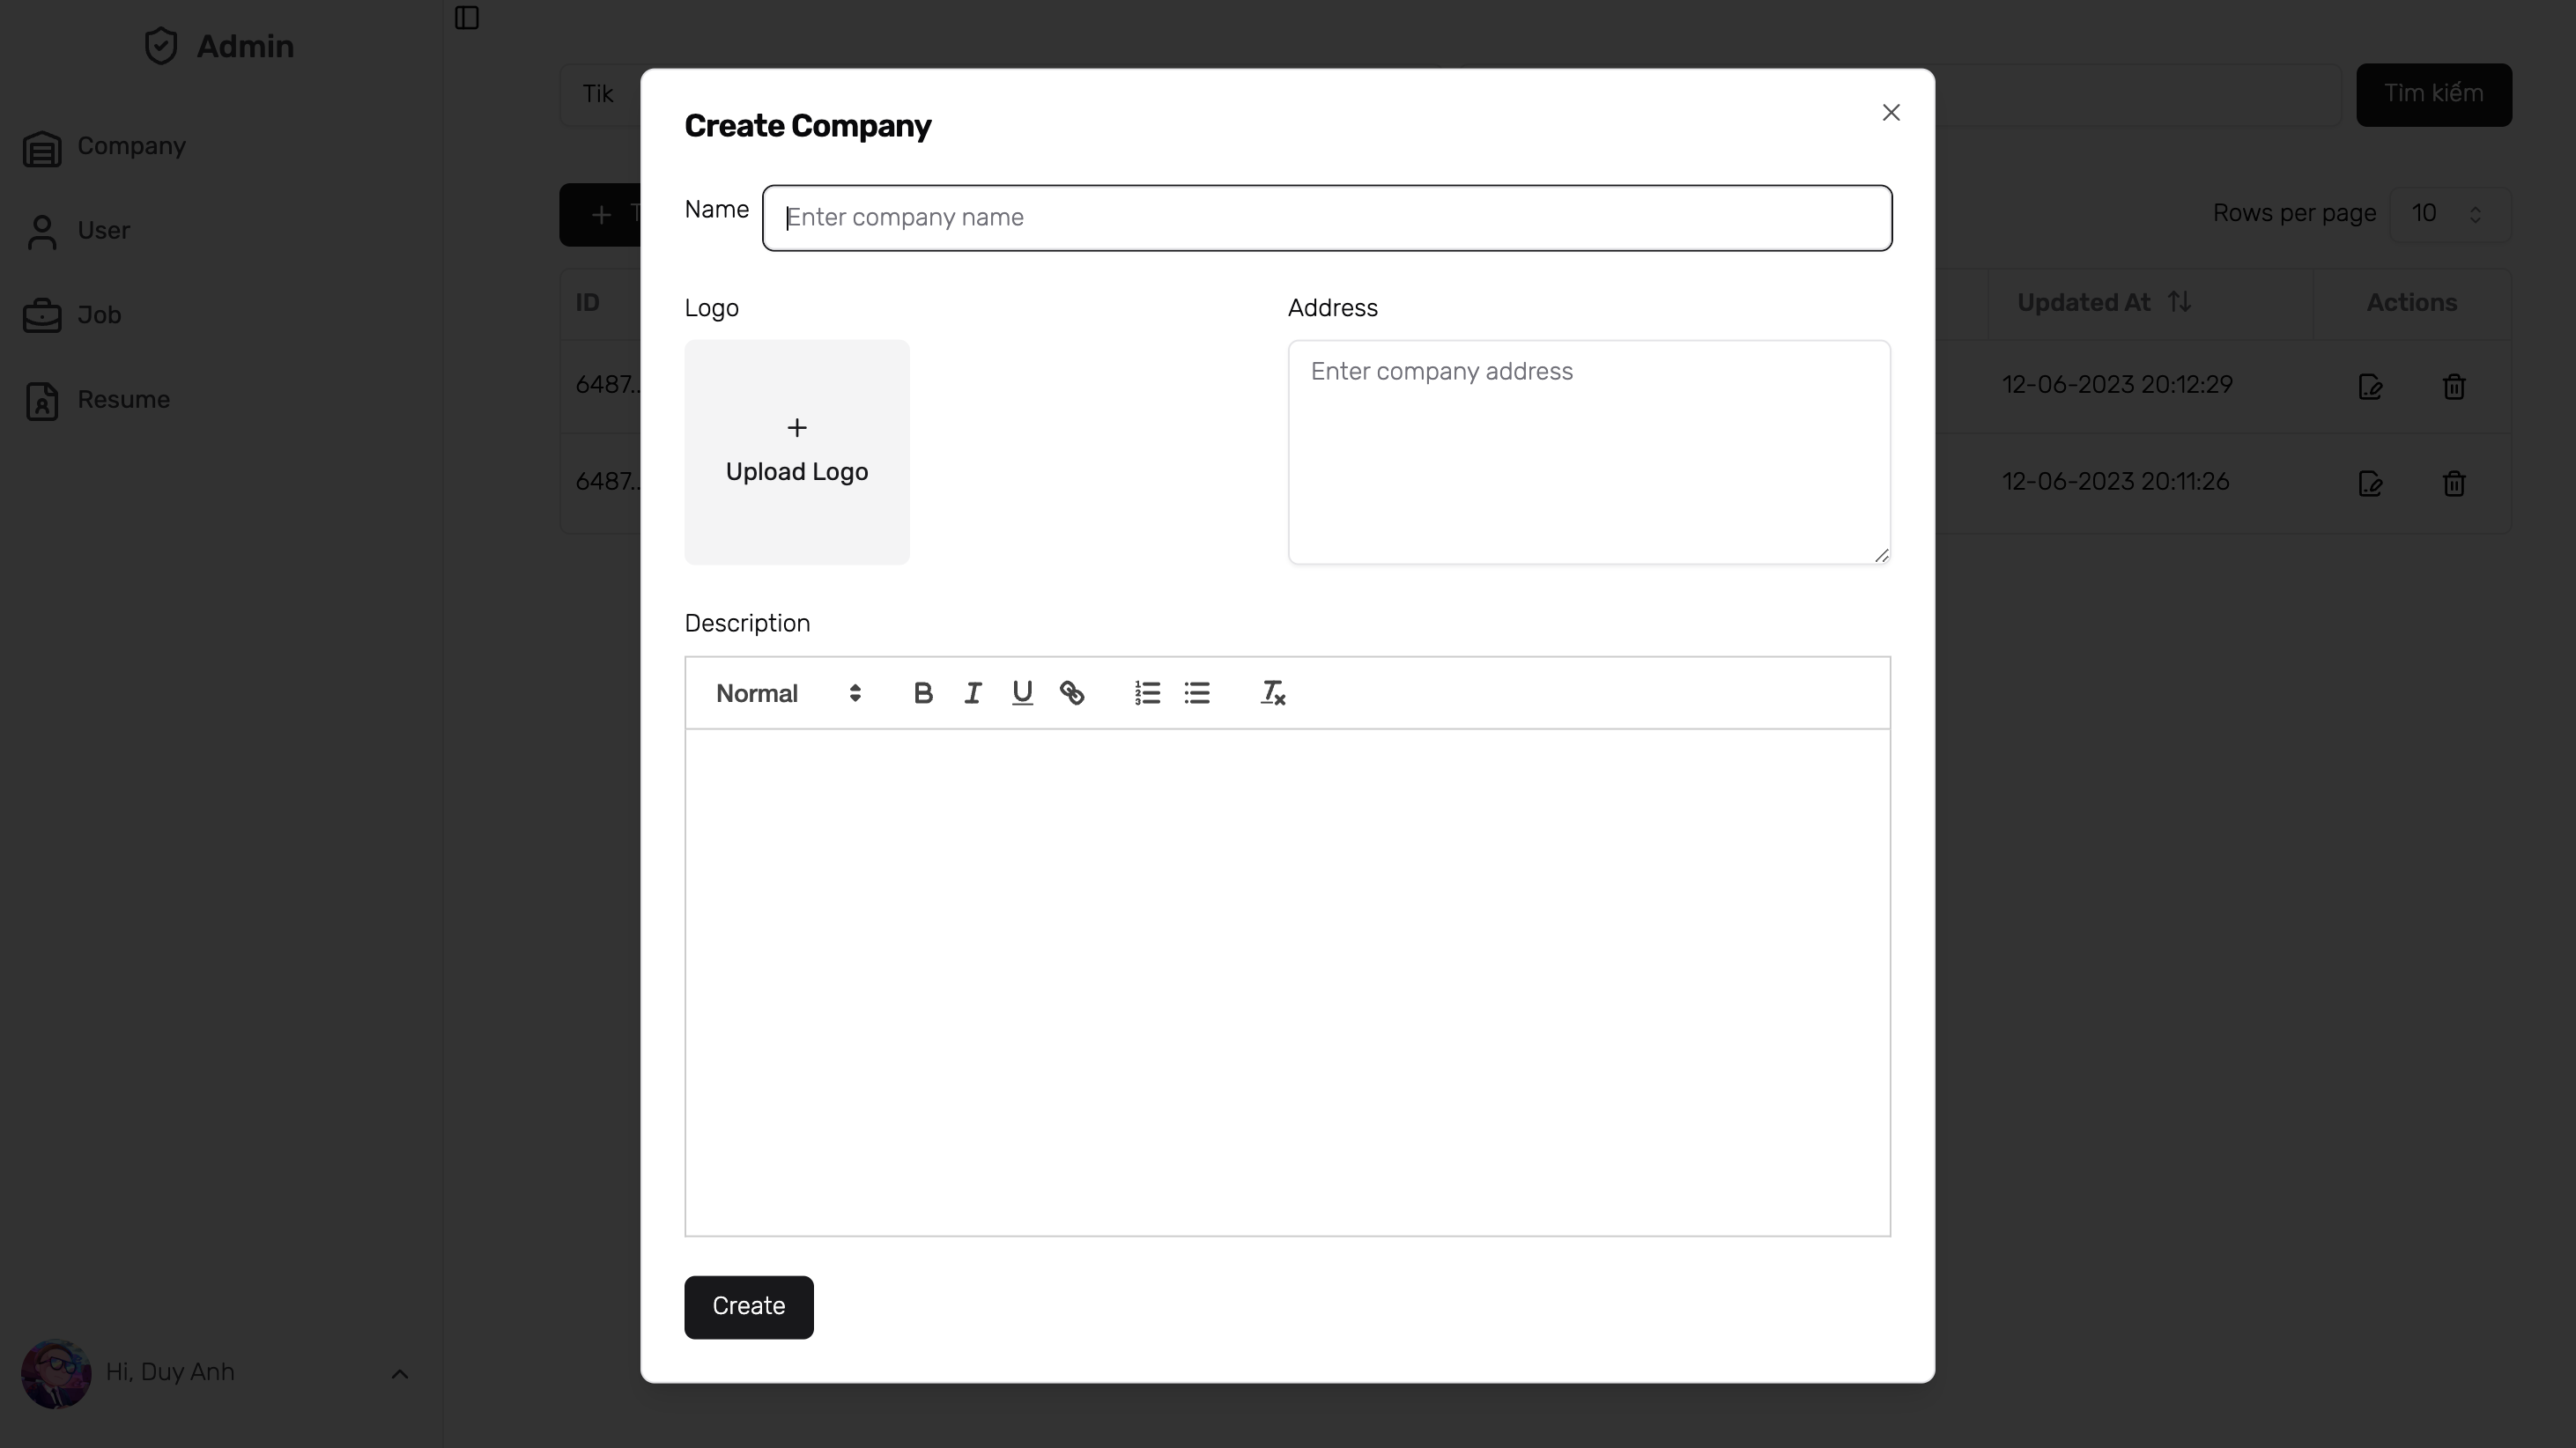
\includegraphics[width=\linewidth]{DBMS-Application/Images/create-company.png}
        \caption{Trang quản lý công ty - Thêm mới công ty}
        \label{fig:enter-label}
    \end{figure}

    \item \textbf{Update}: Cập nhật/chỉnh sửa thông tin công ty cụ thể
    \begin{figure}[H]
        \centering
        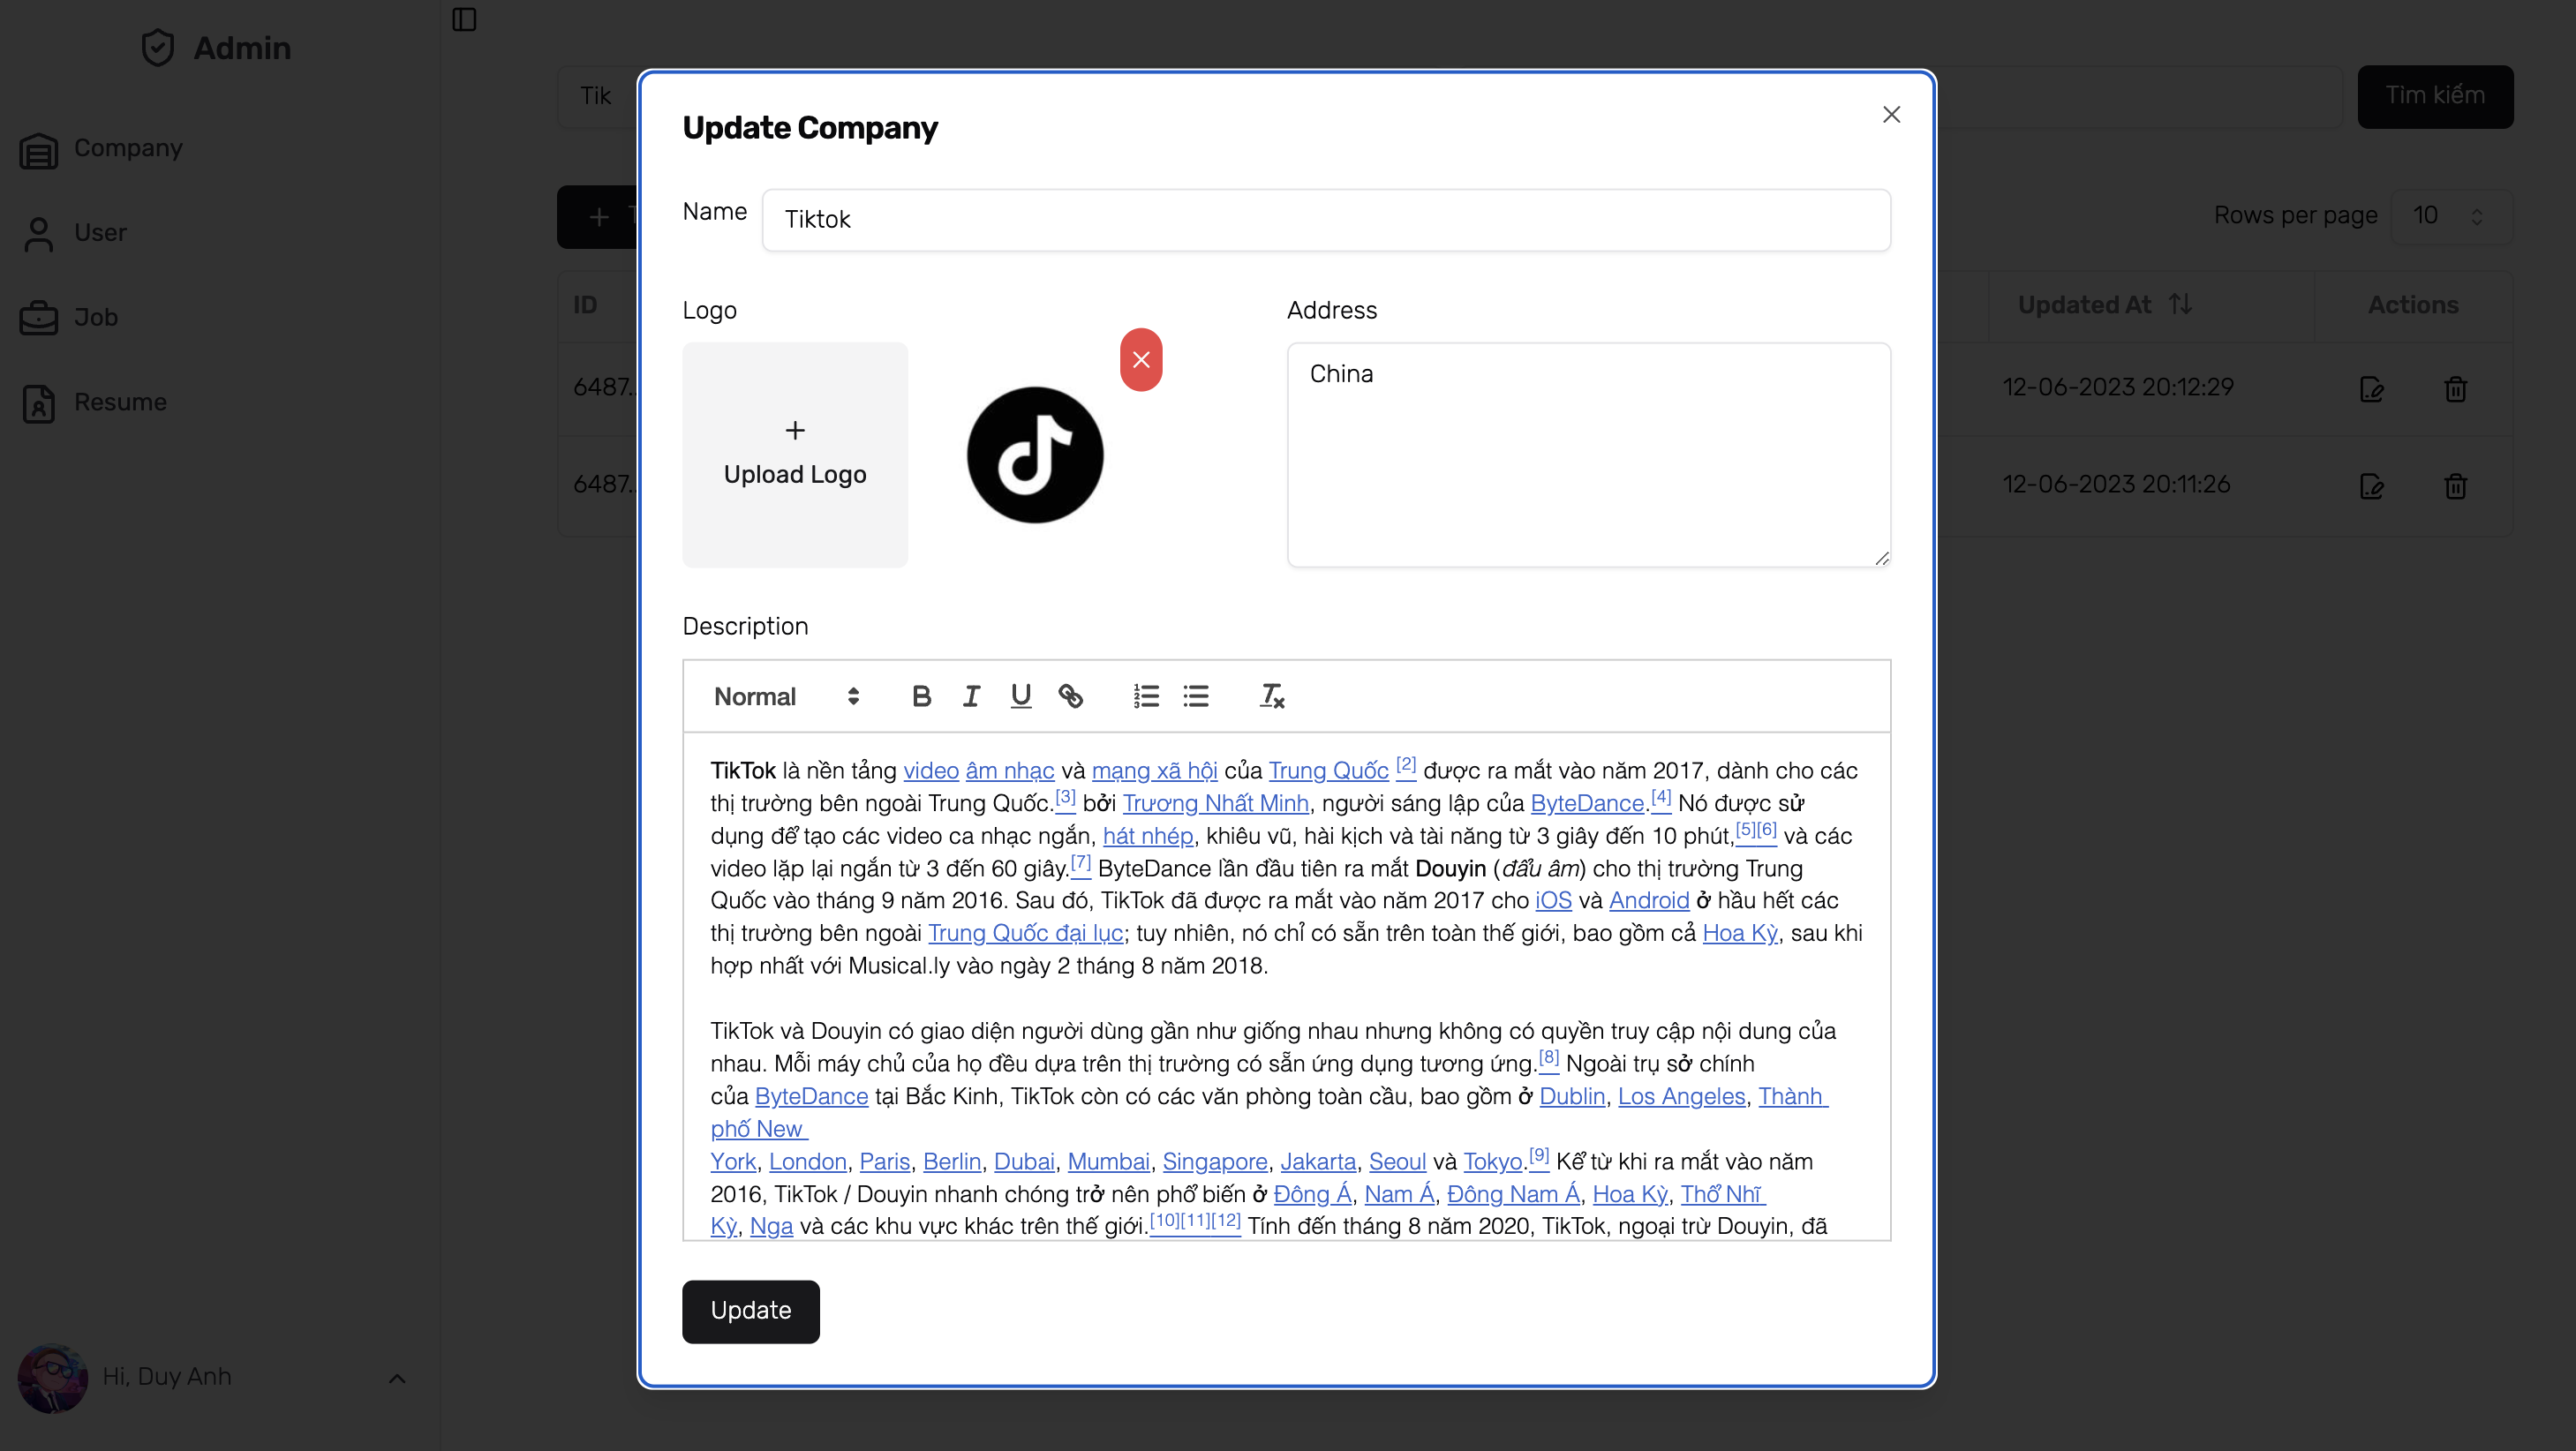
\includegraphics[width=\linewidth]{DBMS-Application/Images/update-company.png}
        \caption{Trang quản lý công ty - Cập nhật thông tin công ty}
        \label{fig:enter-label}
    \end{figure}

    \item \textbf{Delete}: Xoá công ty cụ thể
    \begin{figure}[H]
        \centering
        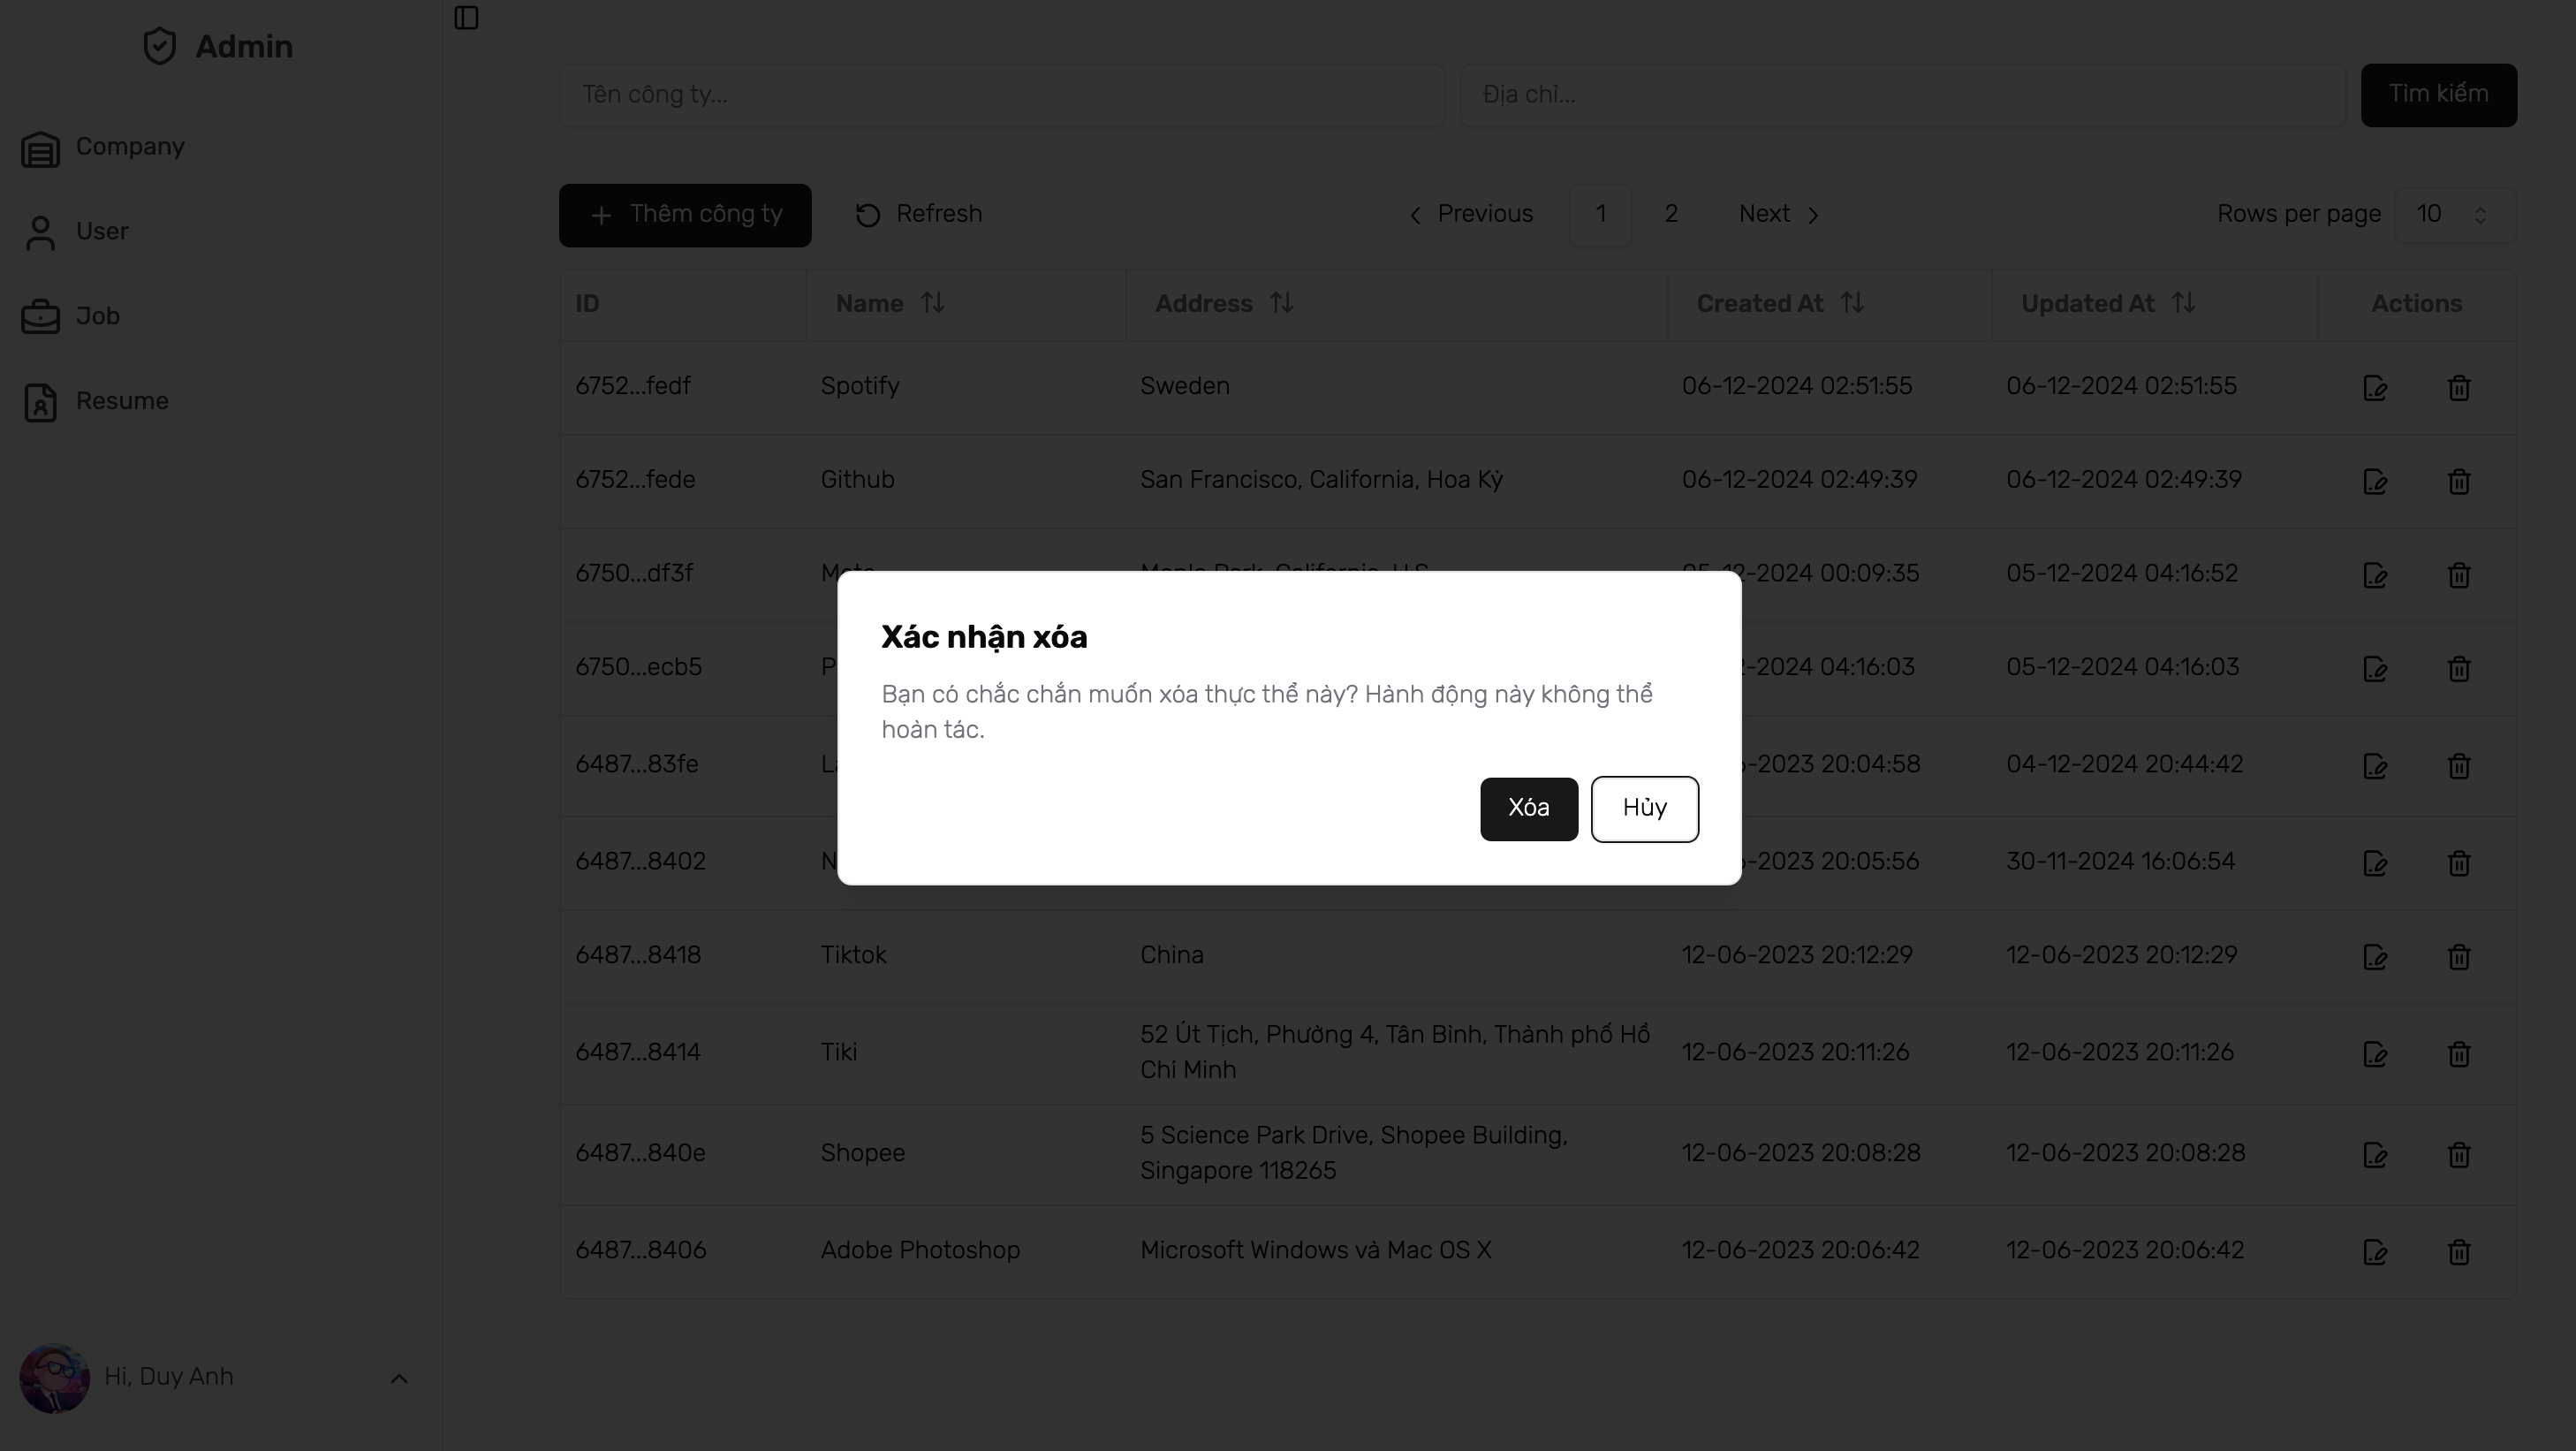
\includegraphics[width=\linewidth]{DBMS-Application/Images/delete-company.png}
        \caption{Trang quản lý công ty - Xoá công ty}
        \label{fig:enter-label}
    \end{figure}
\end{itemize}

% \subsubsection{Giao diện Admin - Quản lý người dùng}

Tương tự với trang quản lý công ty và quản lý công việc, trang quản lý người dùng cũng sử dụng các loại truy vấn sau để hỗ trợ cho các thao tác CRUD:

\begin{itemize}
    \item \textbf{Query with single/composite condition}: Để fetch lên dữ liệu toàn bộ người dùng trong hệ thống theo cơ chế phân trang và một số điều kiện như \textbf{Tên người dùng}, \textbf{Email}
    \begin{figure}[H]
        \centering
        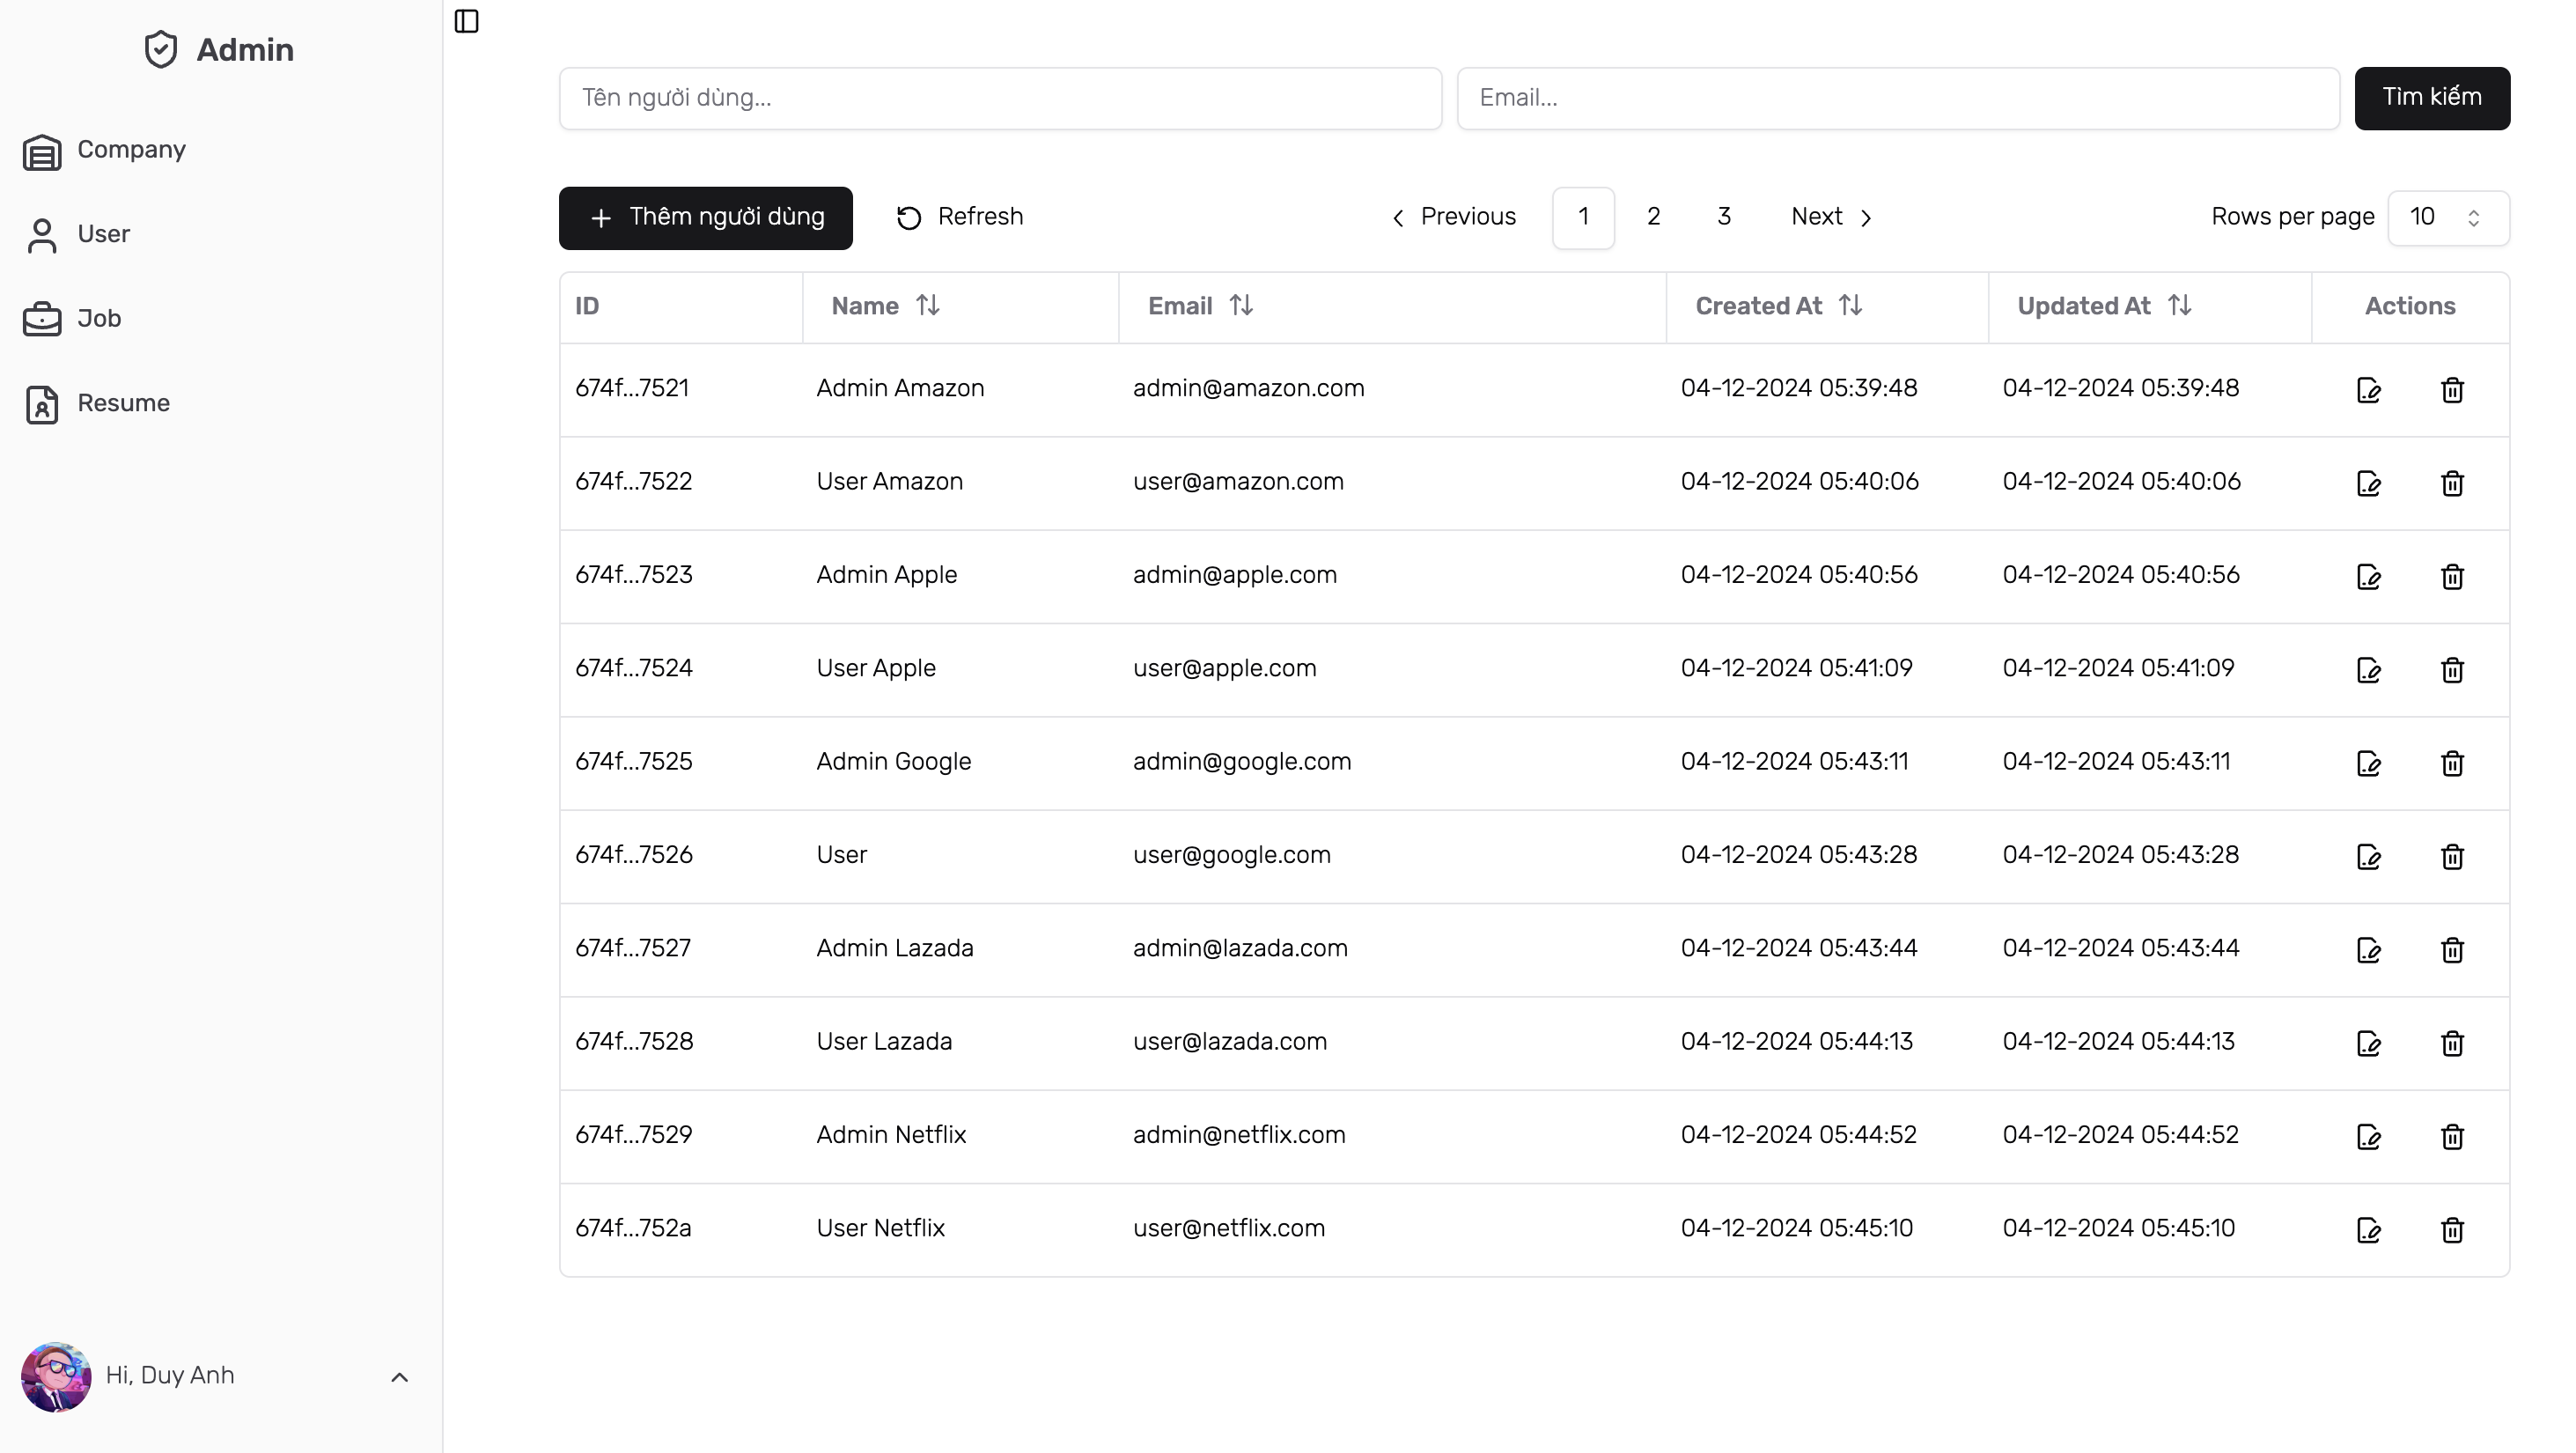
\includegraphics[width=\linewidth]{DBMS-Application/Images/admin-user.png}
        \caption{Trang quản lý người dùng - Danh sách người dùng trong hệ thống}
        \label{fig:enter-label}
    \end{figure}
    
    \item \textbf{Insert}: Thêm mới một người dùng
    \begin{figure}[H]
        \centering
        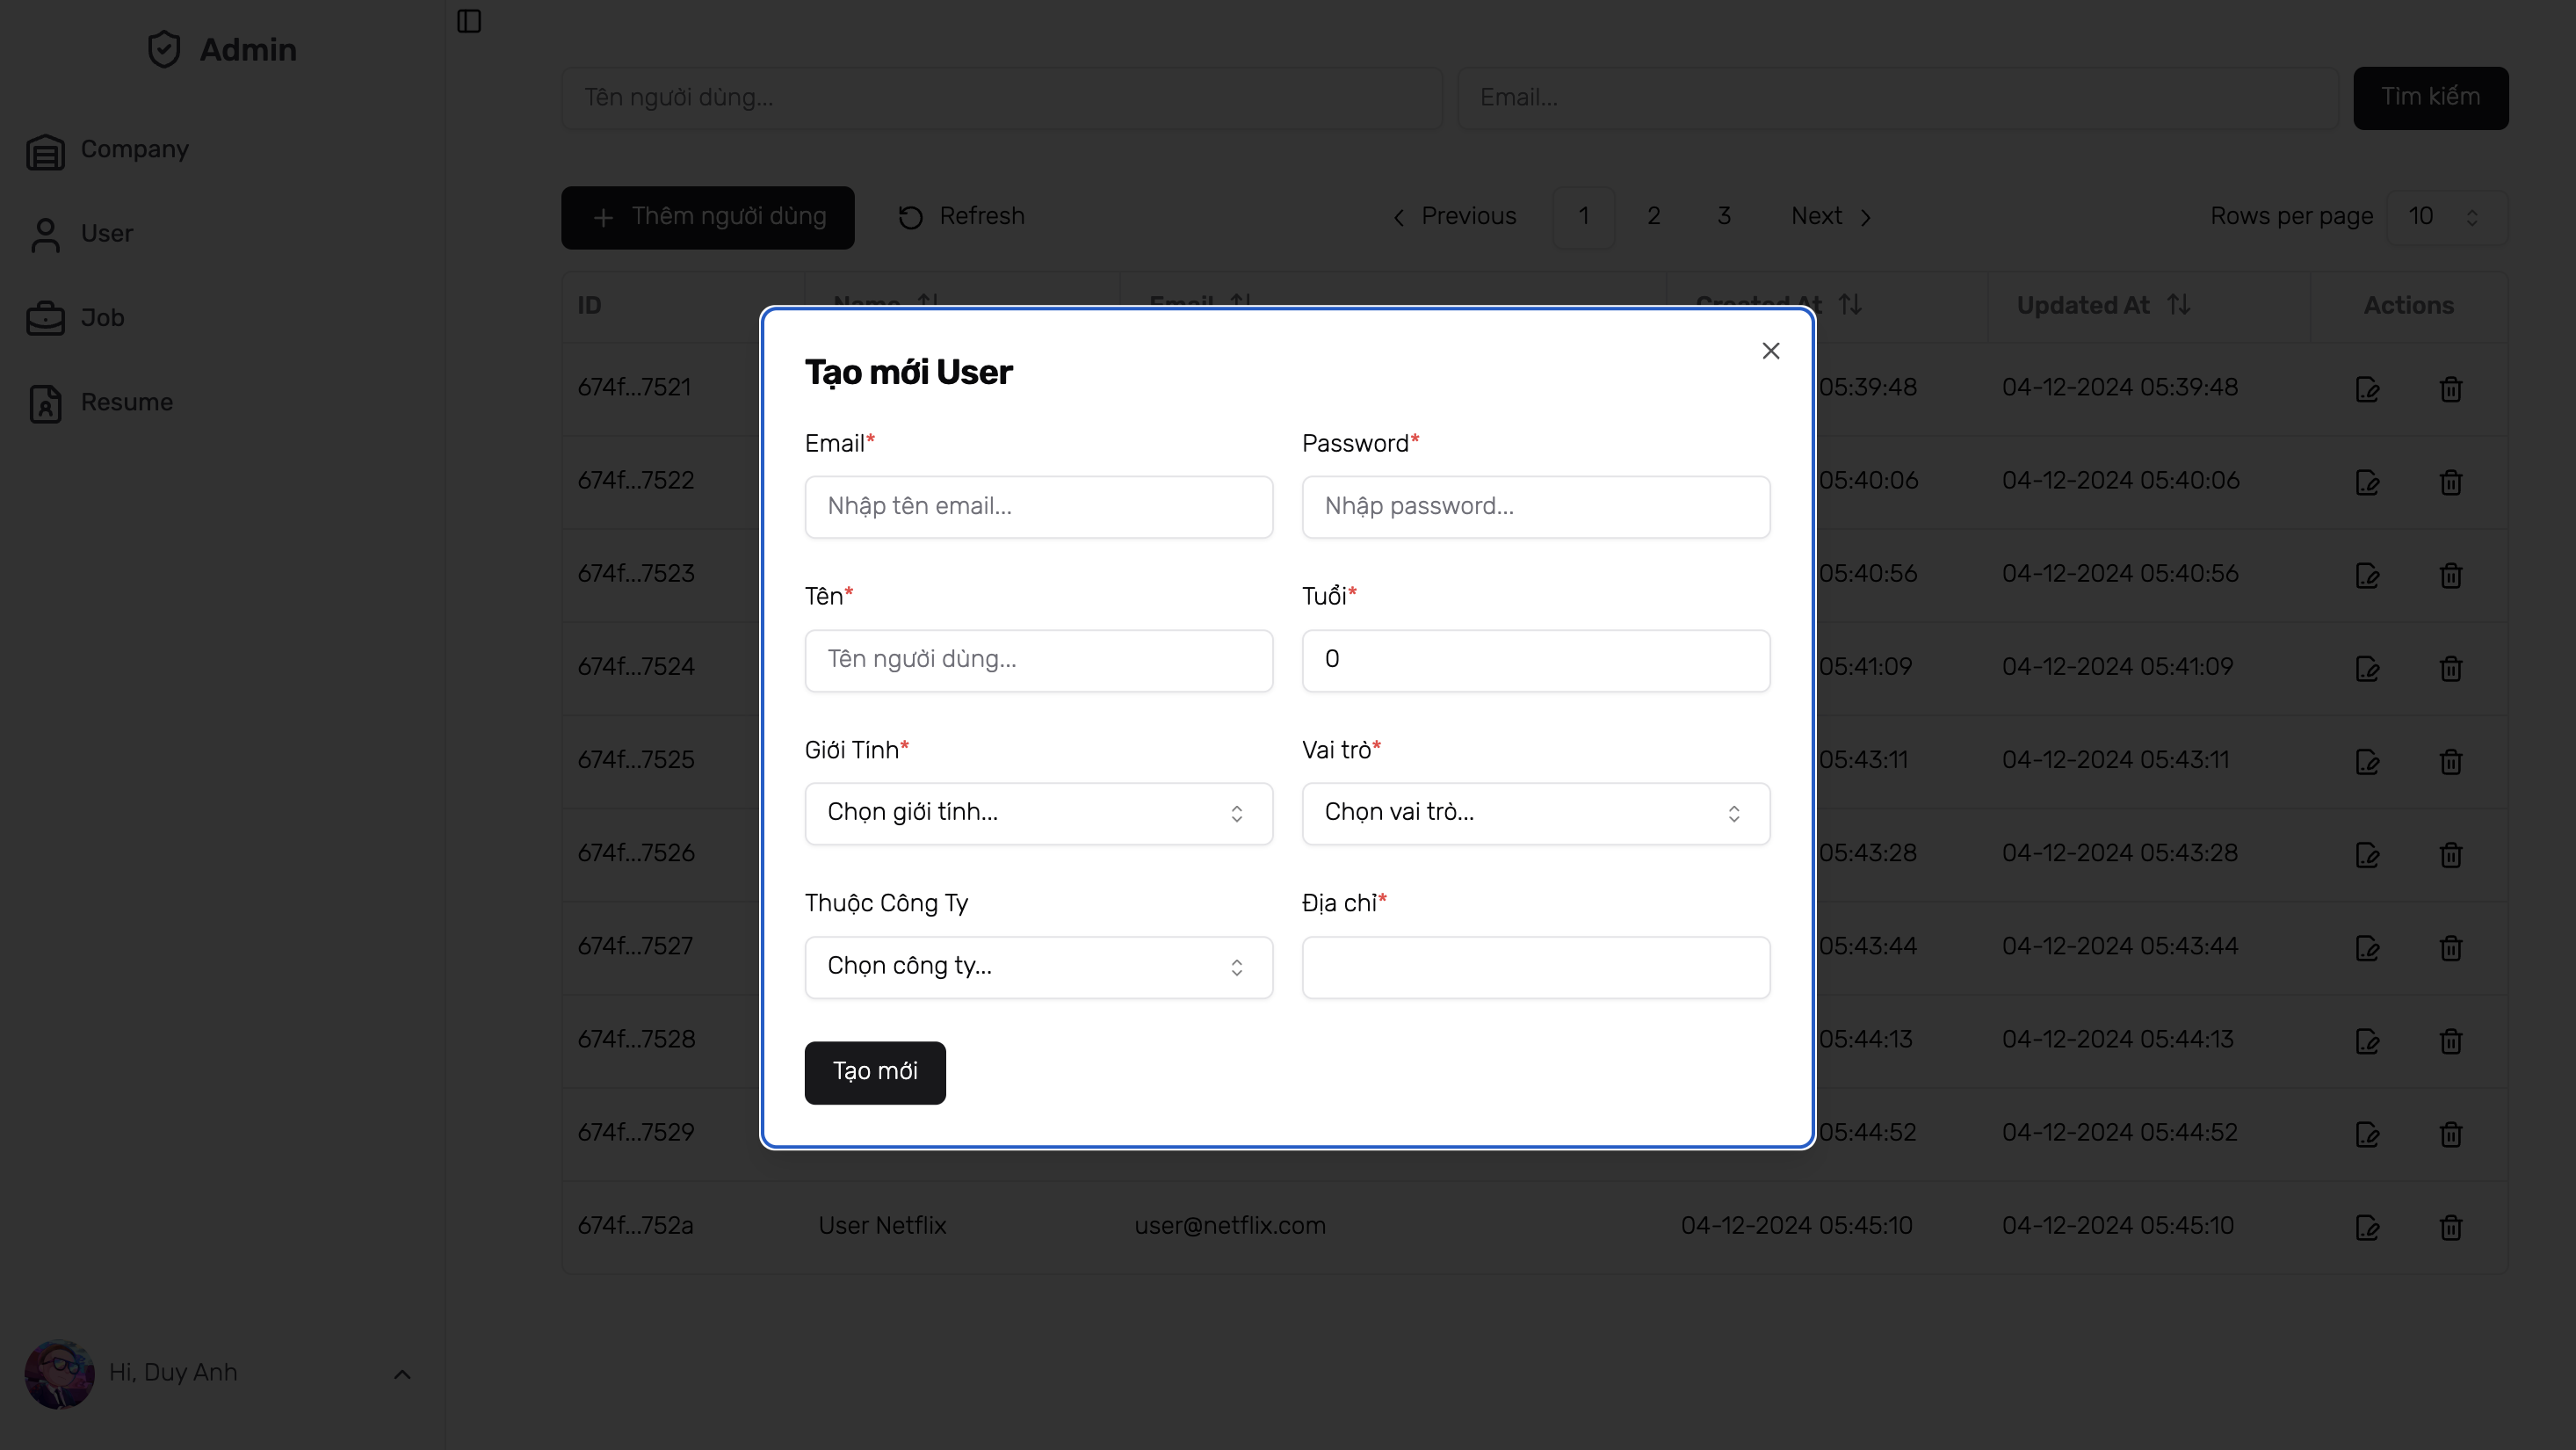
\includegraphics[width=\linewidth]{DBMS-Application/Images/create-user.png}
        \caption{Trang quản lý người dùng - Thêm mới người dùng}
        \label{fig:enter-label}
    \end{figure}

    \item \textbf{Update}: Cập nhật/chỉnh sửa thông tin người dùng cụ thể
    \begin{figure}[H]
        \centering
        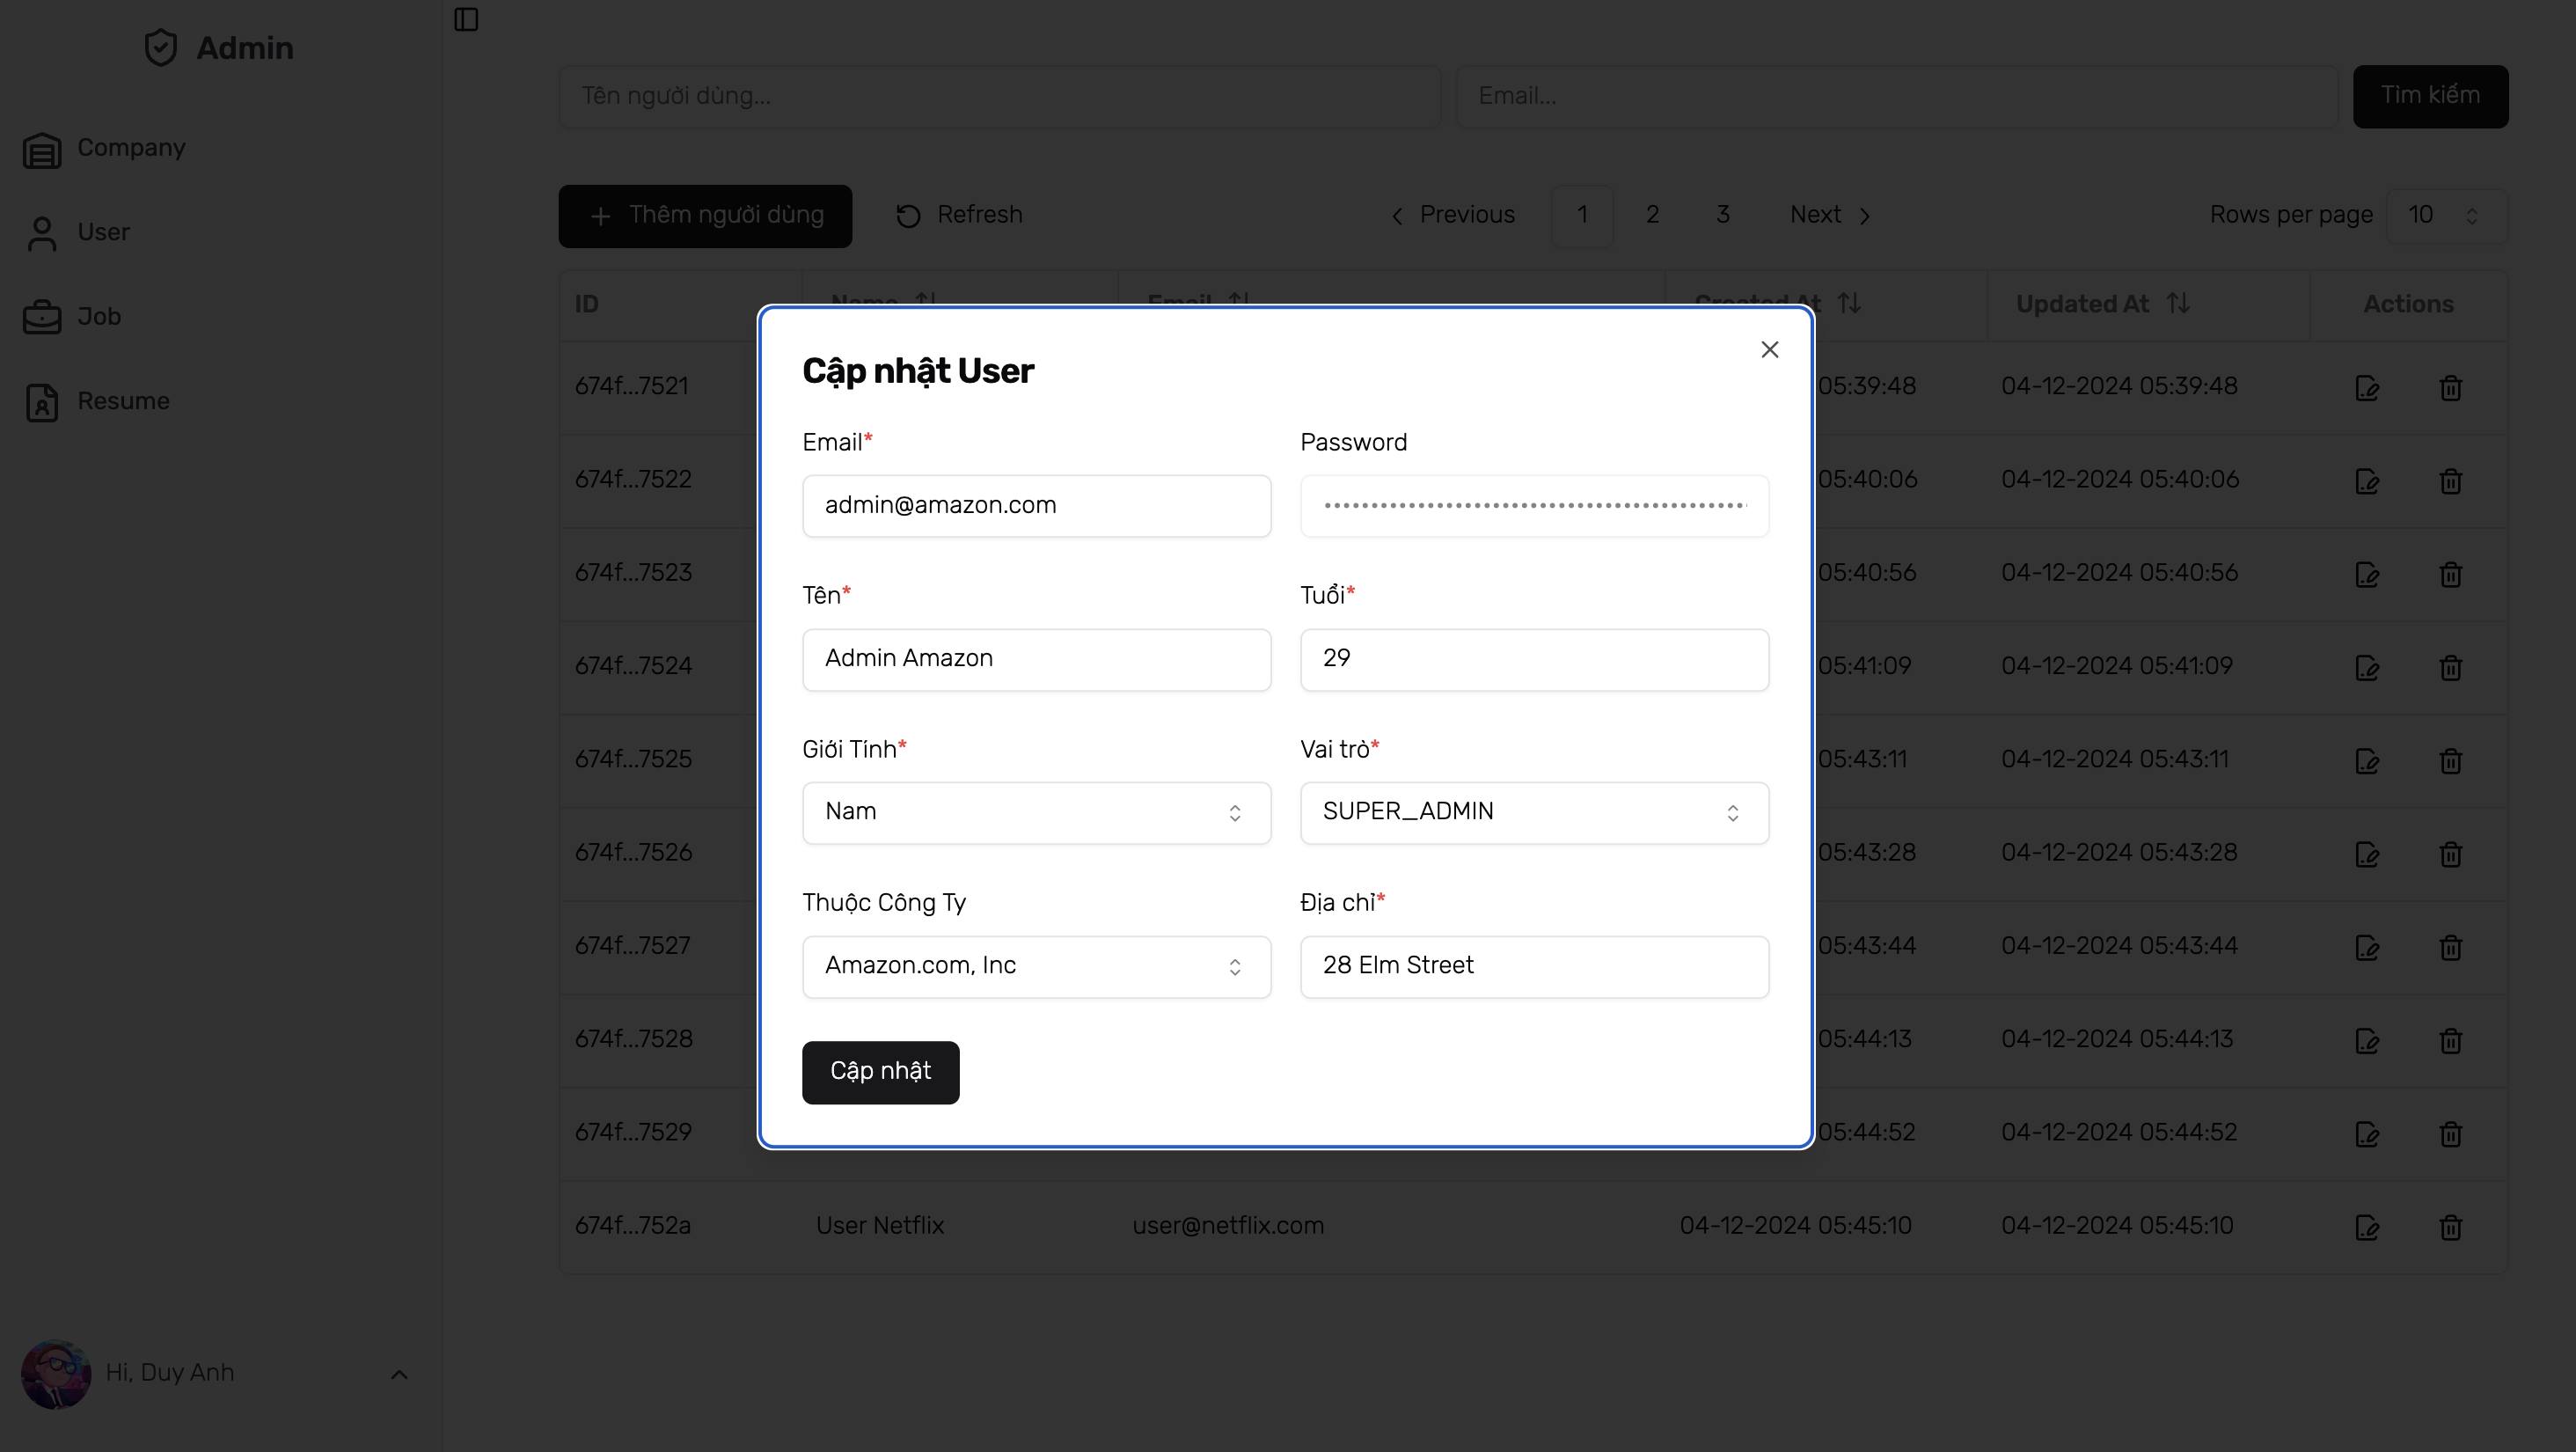
\includegraphics[width=\linewidth]{DBMS-Application/Images/update-user.png}
        \caption{Trang quản lý người dùng - Cập nhật thông tin người dùng}
        \label{fig:enter-label}
    \end{figure}

    \item \textbf{Delete}: Xoá người dùng
    \begin{figure}[H]
        \centering
        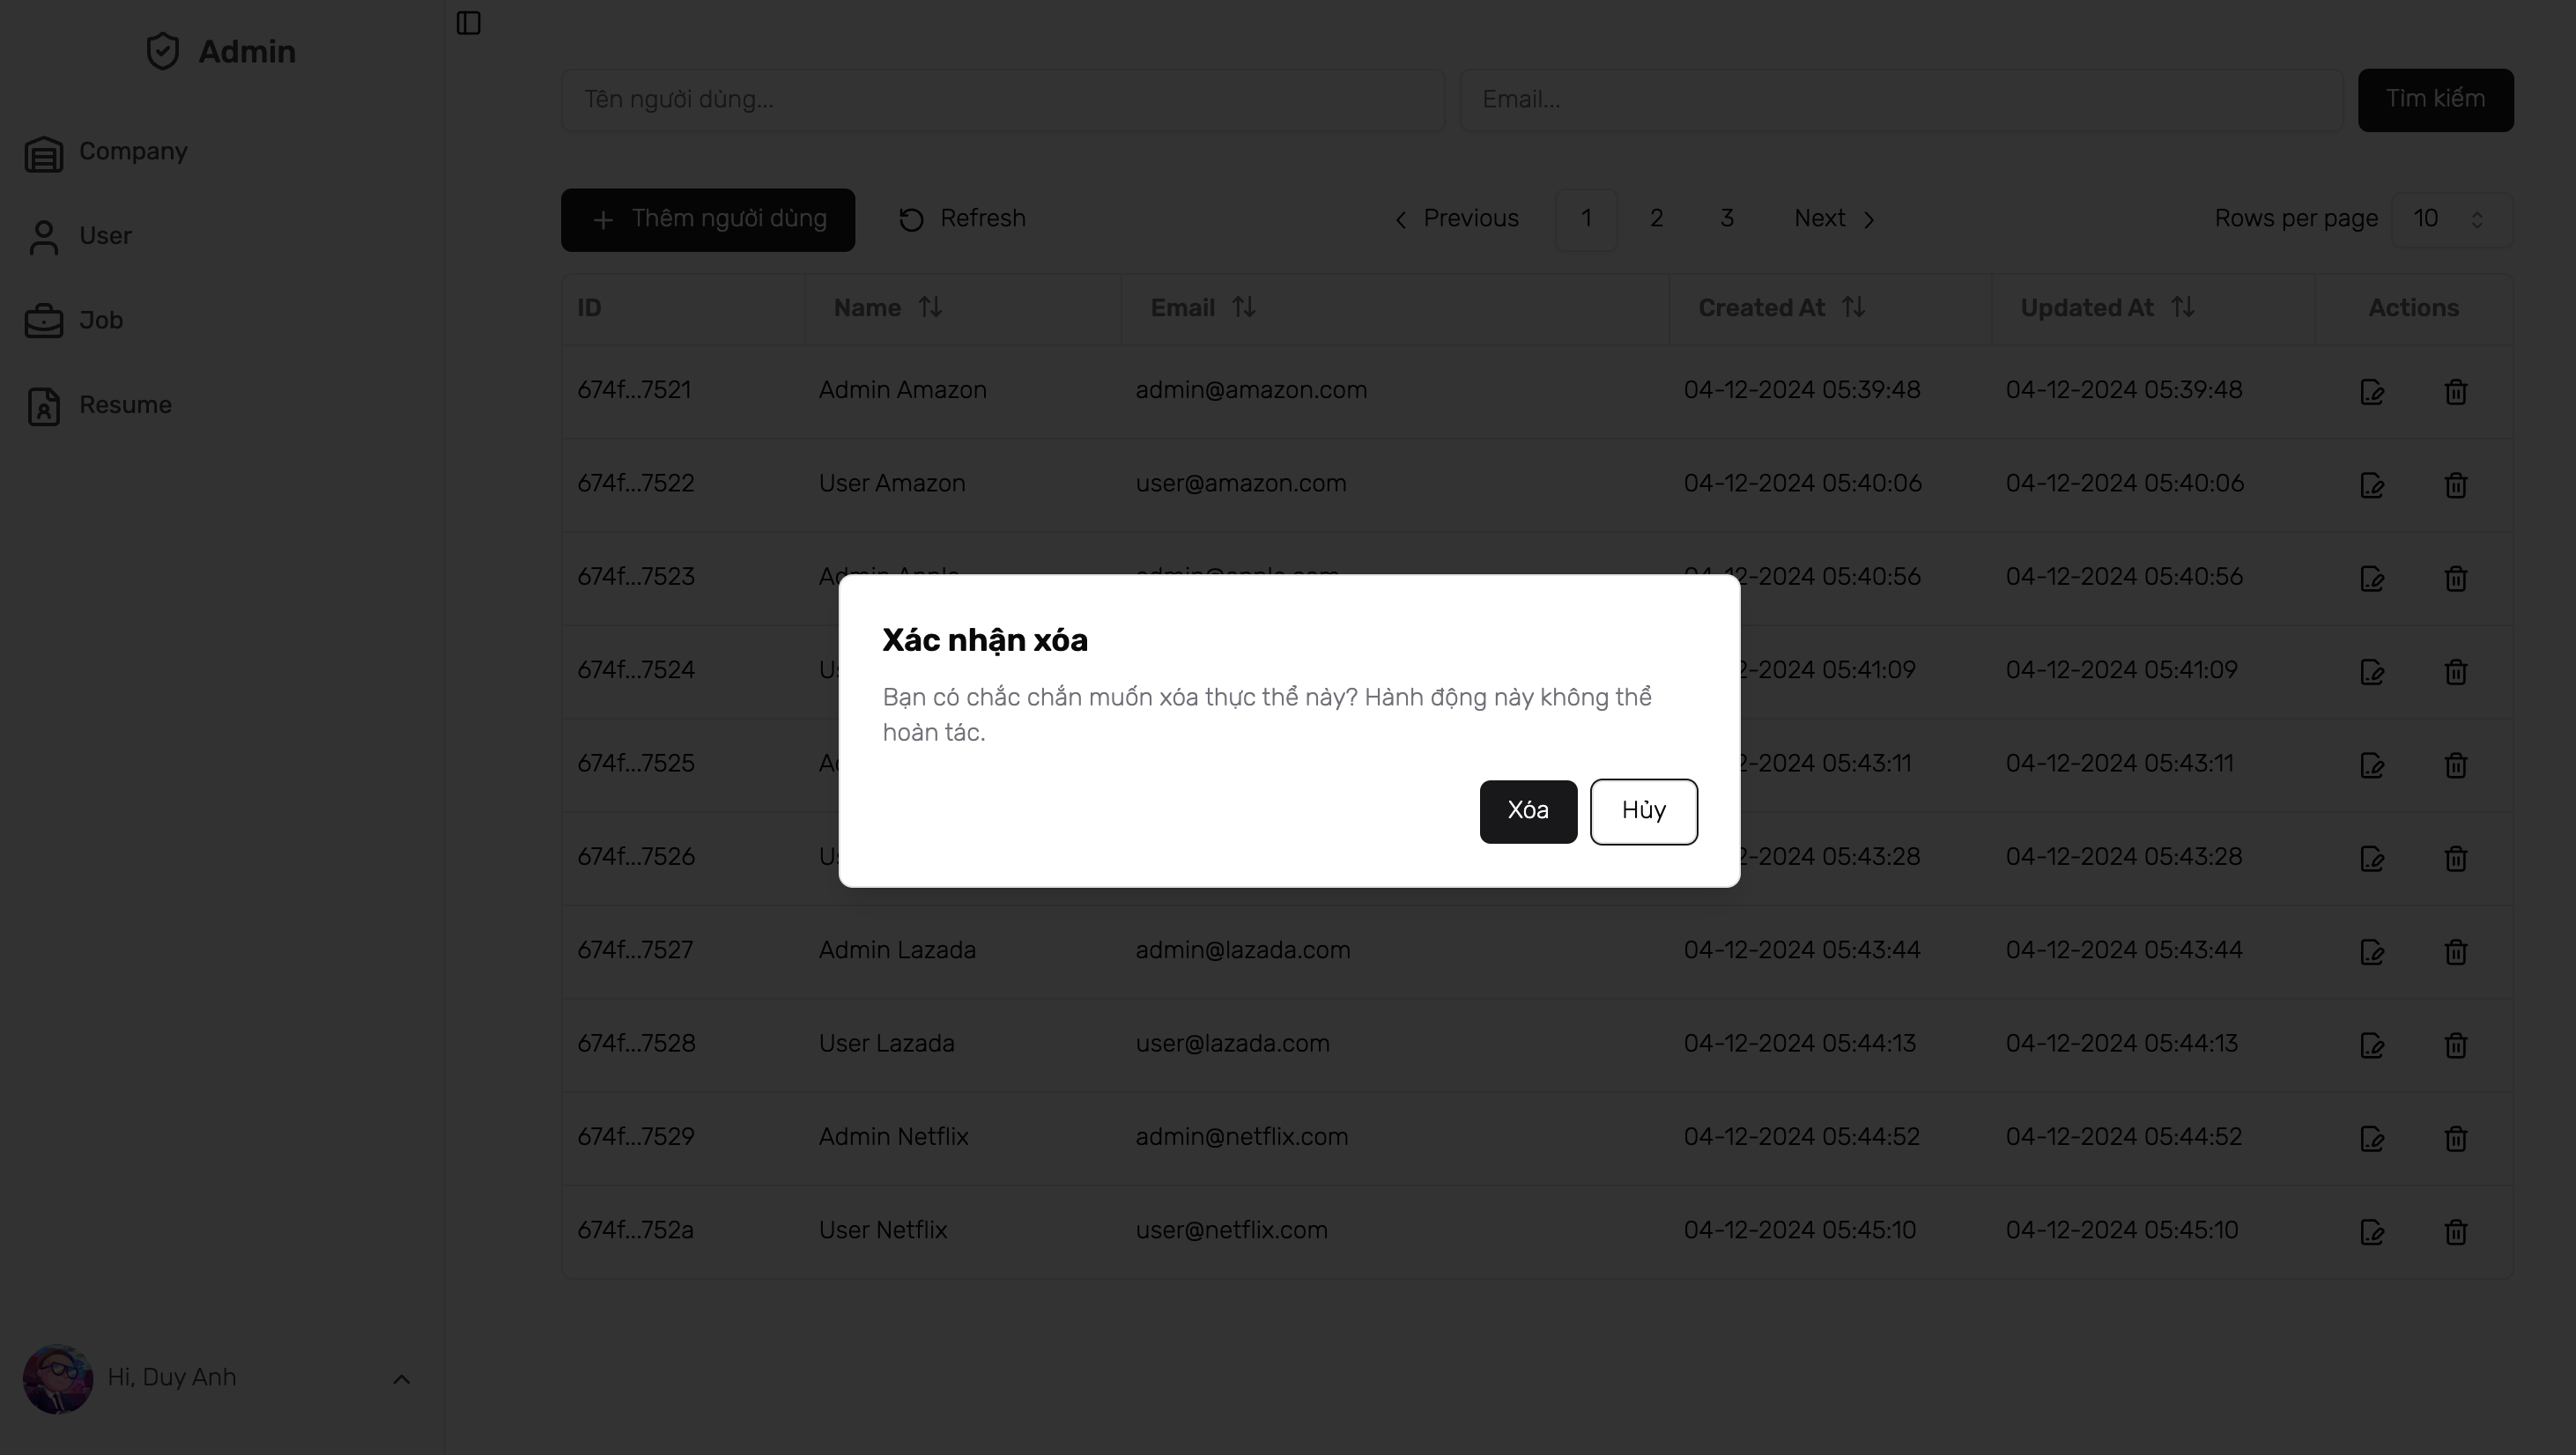
\includegraphics[width=\linewidth]{DBMS-Application/Images/delete-user.png}
        \caption{Trang quản lý người dùng - Xoá người dùng}
        \label{fig:enter-label}
    \end{figure}
\end{itemize}

% \subsubsection{Giao diện Admin - Quản lý hồ sơ ứng tuyển}

\begin{itemize}
    \item \textbf{Query with composite condition}: Để fetch lên dữ liệu toàn bộ hồ sơ ứng tuyển trong hệ thống theo cơ chế phân trang
    \begin{figure}[H]
        \centering
        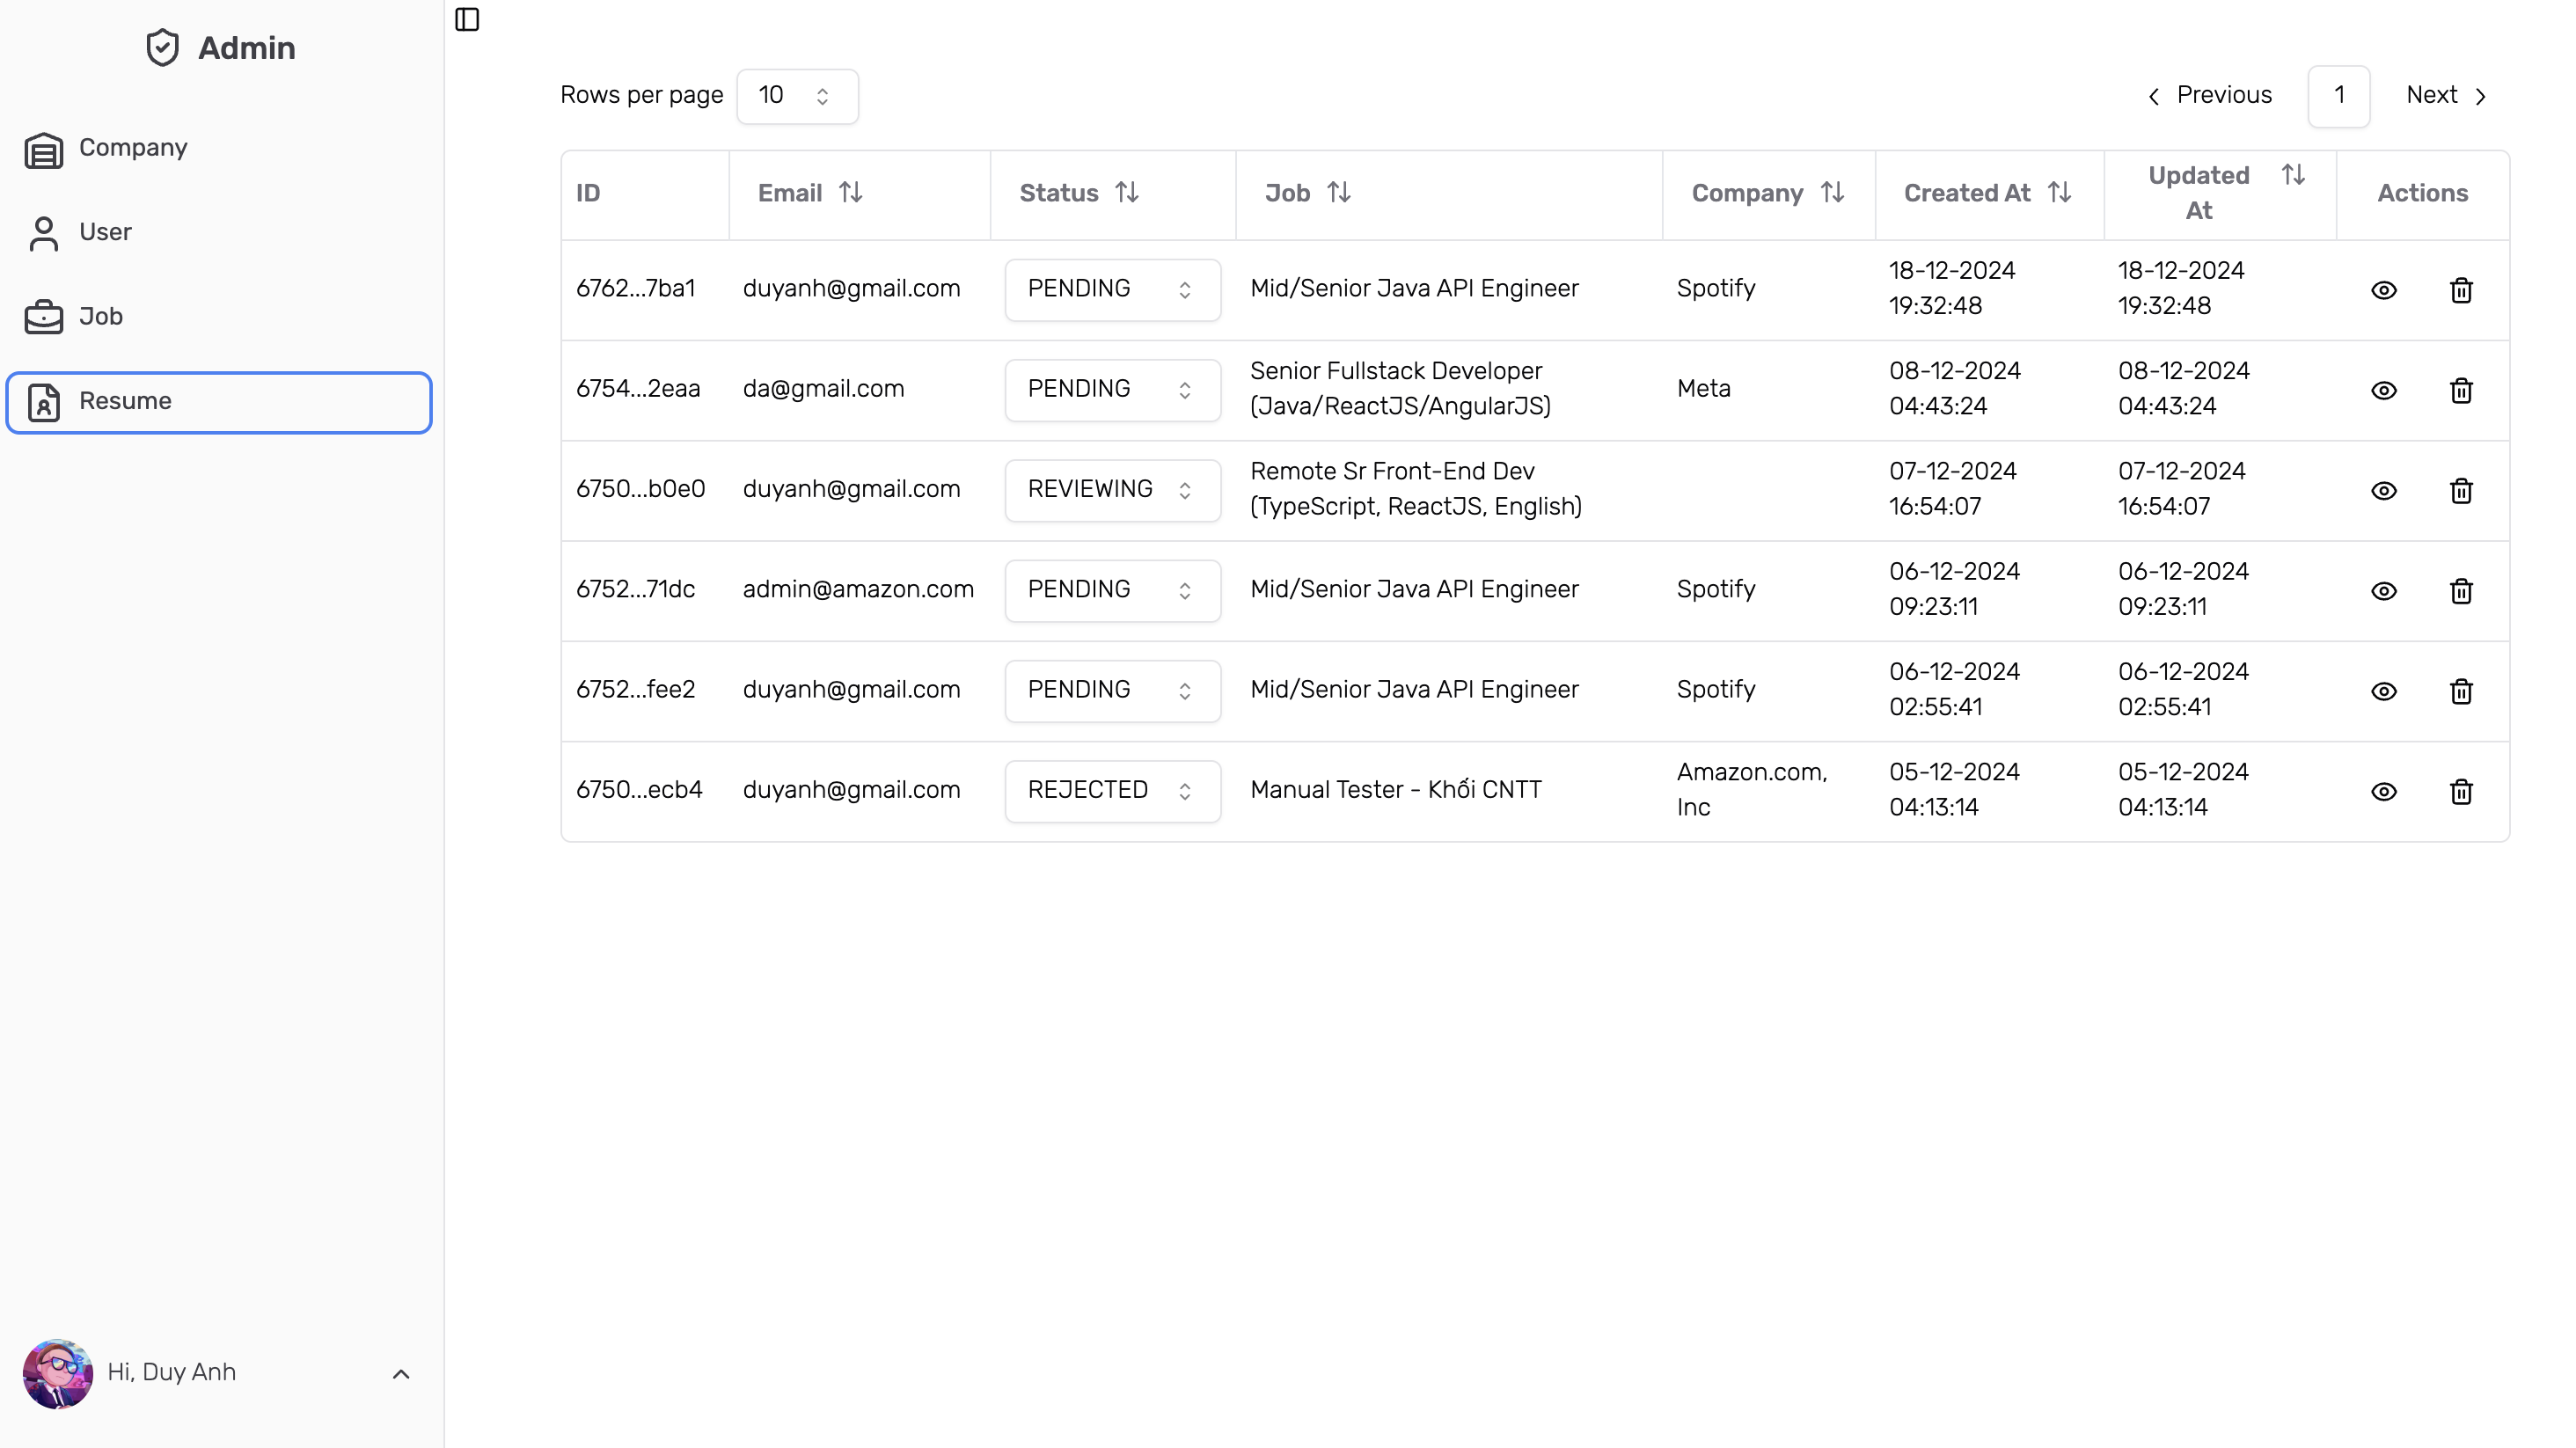
\includegraphics[width=\linewidth]{DBMS-Application/Images/admin-resume.png}
        \caption{Trang quản lý hồ sơ ứng tuyển - Danh sách hồ sơ ứng tuyển trong hệ thống}
        \label{fig:enter-label}
    \end{figure}

    \item \textbf{Update}: Cập nhật thông tin của hồ sơ ứng tuyển, cụ thể là cập nhật \textbf{trạng thái}
    \begin{figure}[H]
        \centering
        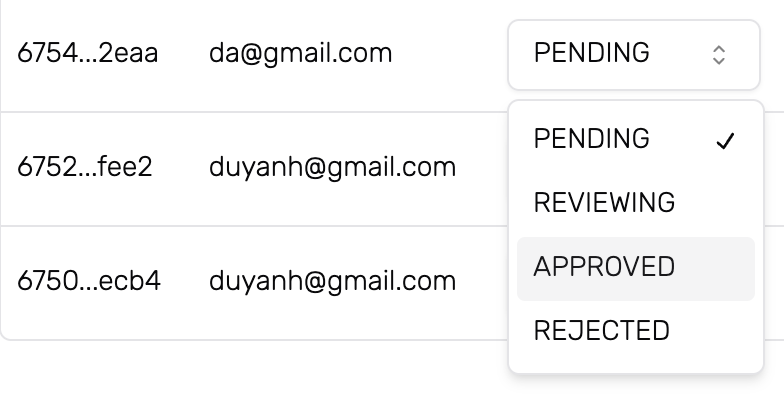
\includegraphics[width=.5\linewidth]{DBMS-Application/Images/update-status-resume.png}
        \caption{Trang quản lý hồ sơ ứng tuyển - Chọn trạng thái mới cho hồ sơ}
        \label{fig:enter-label}
    \end{figure}

    \begin{figure}[H]
        \centering
        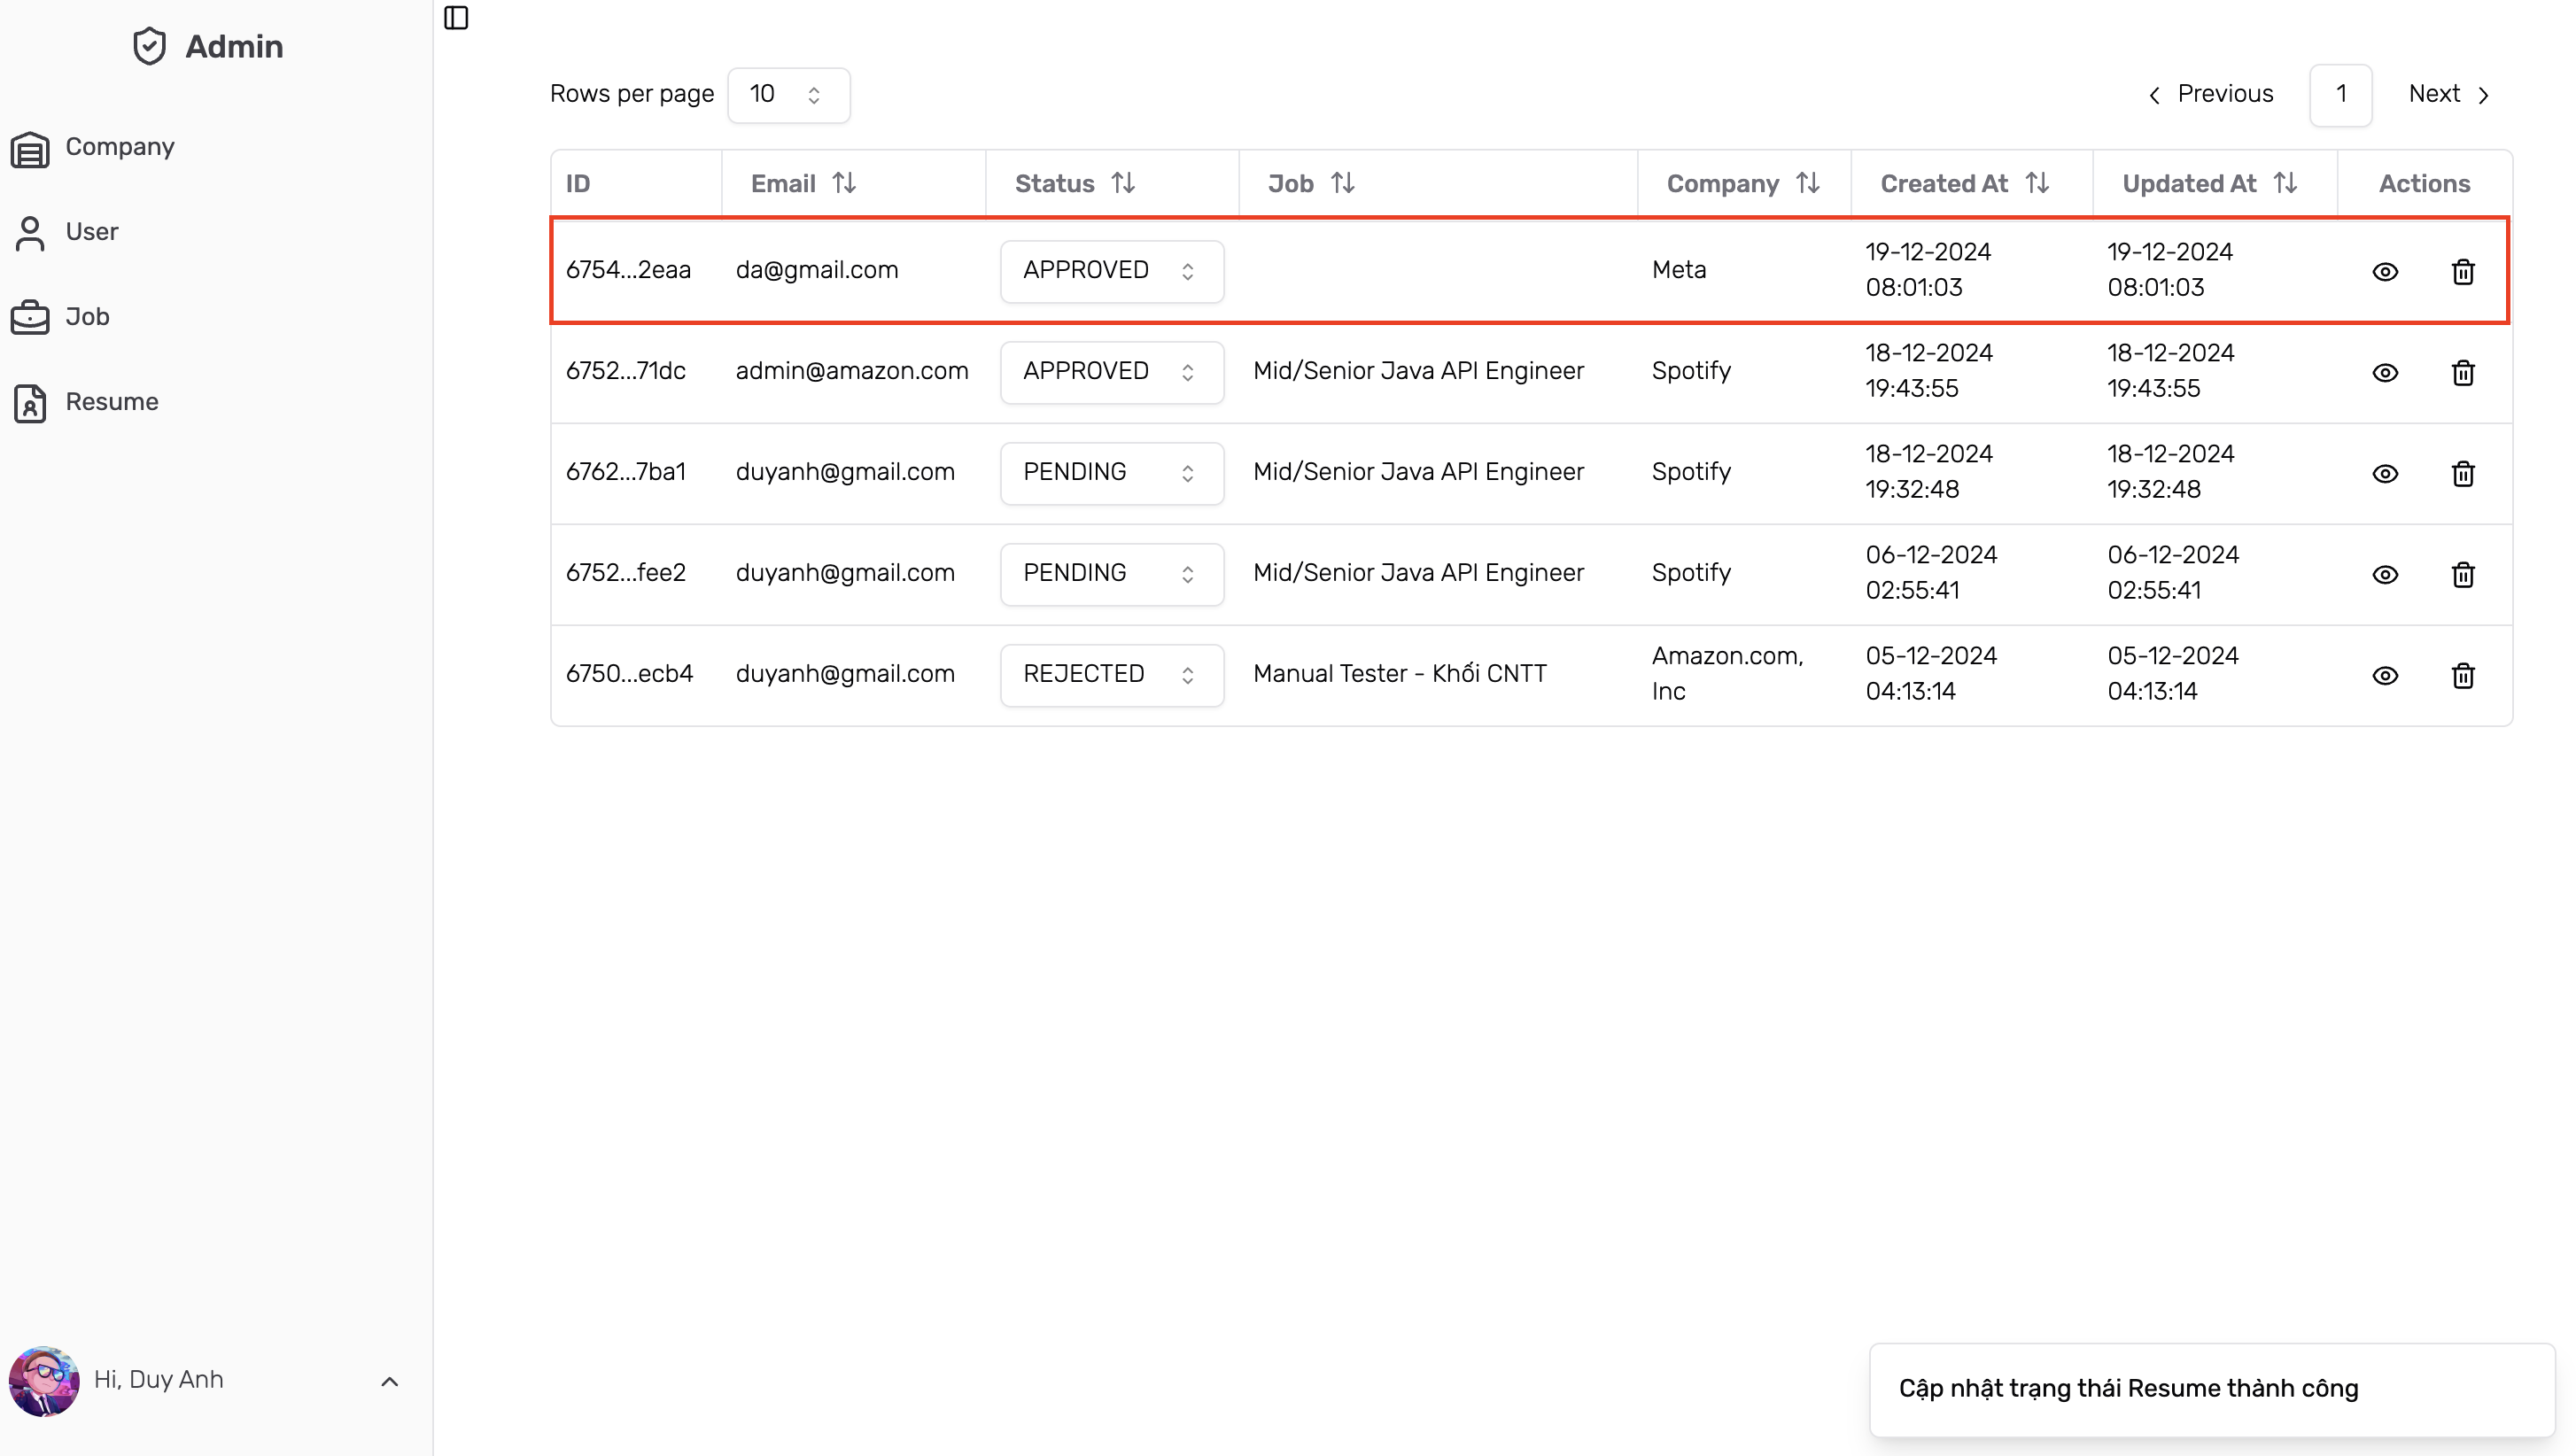
\includegraphics[width=\linewidth]{DBMS-Application/Images/update-resume-successfully.png}
        \caption{Trang quản lý hồ sơ ứng tuyển - Cập nhật trạng thái của hồ sơ ứng tuyển thành công}
        \label{fig:enter-label}
    \end{figure}
    
    \item \textbf{Delete}: Xoá hồ sơ ứng tuyển chỉ định
    \begin{figure}[H]
        \centering
        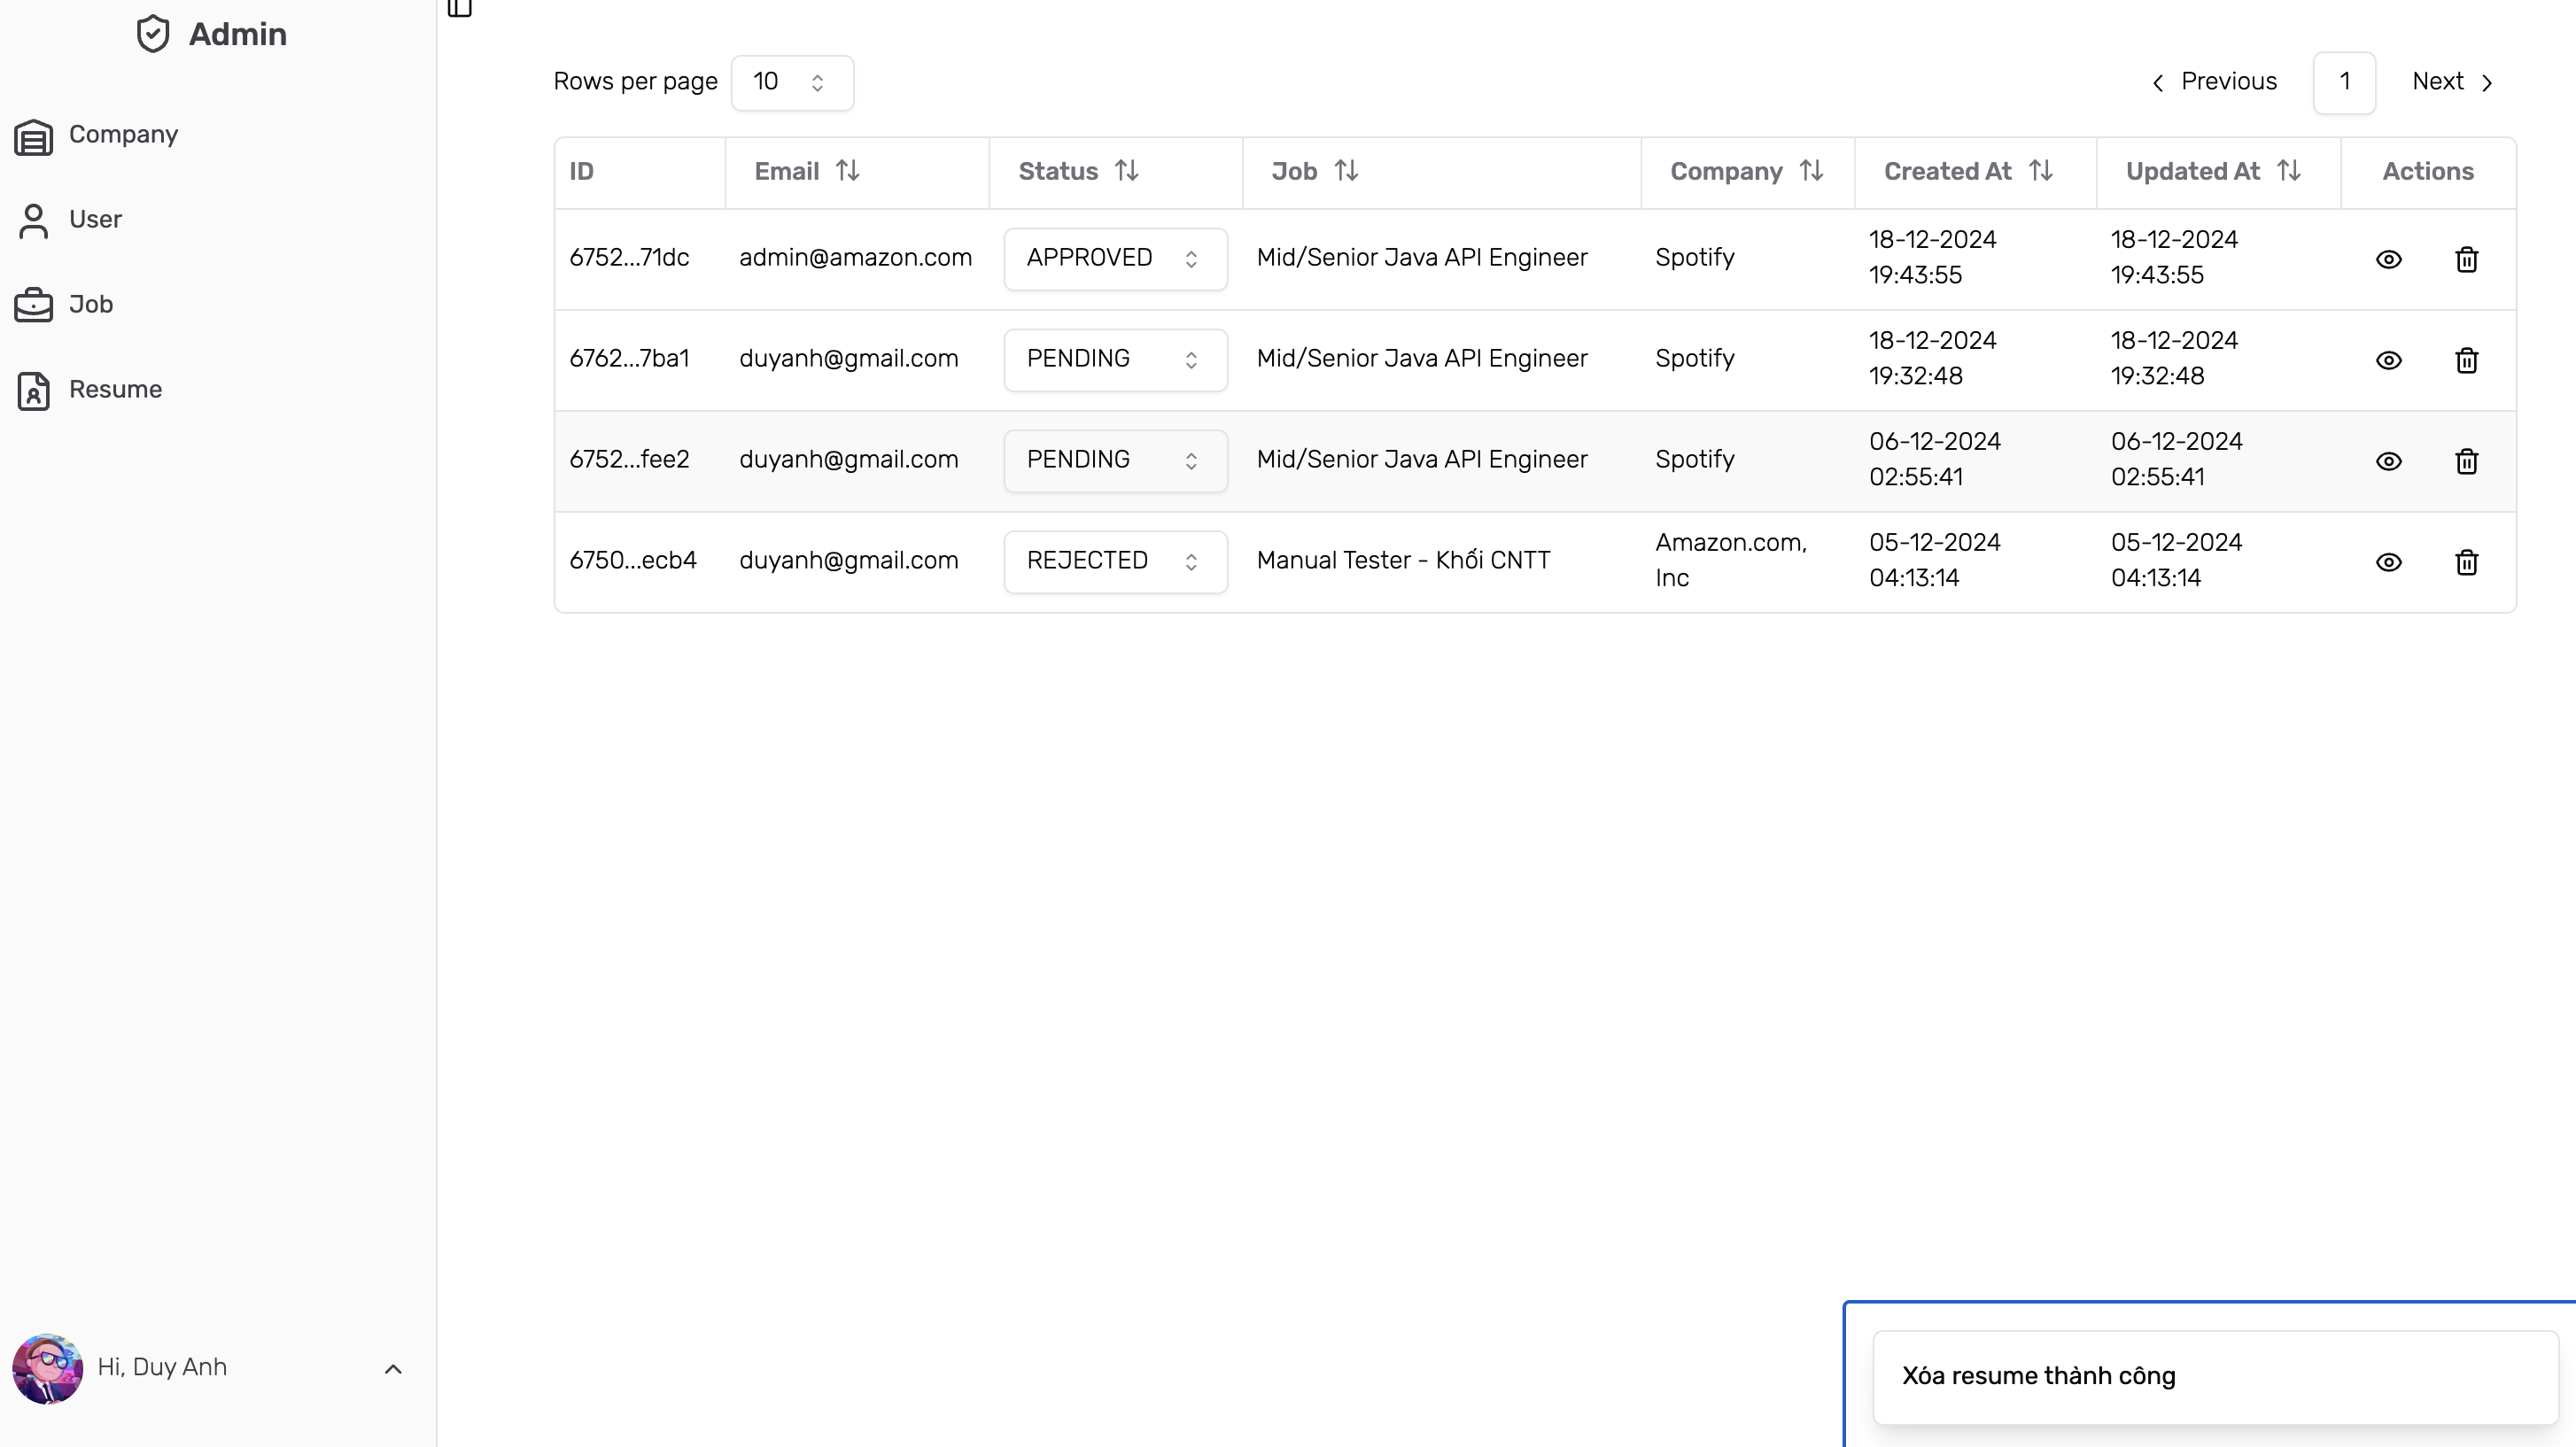
\includegraphics[width=\linewidth]{DBMS-Application/Images/delete-resume.png}
        \caption{Trang quản lý hồ sơ ứng tuyển - Xoá hồ sơ ứng tuyển}
        \label{fig:enter-label}
    \end{figure}
\end{itemize}